\documentclass[bachelor_thesis]{subfiles}

\begin{document}
\chapter{Theoretical background} \label{chap:theory}
\section{Plasma Wakefield acceleration}
\Gls{pwfa} is a novel particle accelerator concept \cite{Chen1985} with the possibility to produce high accelerating electric fields (more than \qty{100}{\giga\volt/\m}). This allows for higher energy gains per meter
and thus several order of magnitude smaller accelerators, compared to conventional \gls{rf} accelerators.

\Gls{pwfa} works by sending a bunch of charged particles (also called drive beam or driver) with relativistic speed ($v_{beam}\approx c$) into a neutral plasma. Multiple sources are possible for this beam and will be further discussed in \autoref{chap:lpfwa}.
In this thesis, the beam consists of electrons but research on other species like positrons \cite{Gessner2016} is made as well. To be easily ionized, the plasma is often formed by light weight gases like lithium (or even hydrogen or helium in newer experiments \cite{Schoebel2022}), 
ionized either by the drive beam itself or a dedicated ionization laser.

When entering the plasma, the drive beam interacts with the plasma electrons, while the effect on the ions can be neglected at the time scale of the electron response. The electric field of the bunch pushes the electrons out of its way, comparable to a snowplow. 
This leaves an electron free cavity behind, starting from the center of the driver while the expelled electrons culminate at the borders of the cavity. As the ions are not moving, this cavity is positively charged, meaning it acts as an attractive force to the plasma electrons.
When being pulled back towards the center of the cavity, the electrons overshoot and produce another cavity. The result is electron oscillation, where multiple cavities form behind the beam as seen in \autoref{fig:pwfa}.

\begin{figure}
	\centering
	%% Creator: Matplotlib, PGF backend
%%
%% To include the figure in your LaTeX document, write
%%   \input{<filename>.pgf}
%%
%% Make sure the required packages are loaded in your preamble
%%   \usepackage{pgf}
%%
%% Also ensure that all the required font packages are loaded; for instance,
%% the lmodern package is sometimes necessary when using math font.
%%   \usepackage{lmodern}
%%
%% Figures using additional raster images can only be included by \input if
%% they are in the same directory as the main LaTeX file. For loading figures
%% from other directories you can use the `import` package
%%   \usepackage{import}
%%
%% and then include the figures with
%%   \import{<path to file>}{<filename>.pgf}
%%
%% Matplotlib used the following preamble
%%
\begingroup%
\makeatletter%
\begin{pgfpicture}%
\pgfpathrectangle{\pgfpointorigin}{\pgfqpoint{6.400000in}{3.000000in}}%
\pgfusepath{use as bounding box, clip}%
\begin{pgfscope}%
\pgfsetbuttcap%
\pgfsetmiterjoin%
\pgfsetlinewidth{0.000000pt}%
\definecolor{currentstroke}{rgb}{1.000000,1.000000,1.000000}%
\pgfsetstrokecolor{currentstroke}%
\pgfsetstrokeopacity{0.000000}%
\pgfsetdash{}{0pt}%
\pgfpathmoveto{\pgfqpoint{0.000000in}{0.000000in}}%
\pgfpathlineto{\pgfqpoint{6.400000in}{0.000000in}}%
\pgfpathlineto{\pgfqpoint{6.400000in}{3.000000in}}%
\pgfpathlineto{\pgfqpoint{0.000000in}{3.000000in}}%
\pgfpathlineto{\pgfqpoint{0.000000in}{0.000000in}}%
\pgfpathclose%
\pgfusepath{}%
\end{pgfscope}%
\begin{pgfscope}%
\pgfpathrectangle{\pgfqpoint{0.640000in}{0.150000in}}{\pgfqpoint{5.120000in}{2.700000in}}%
\pgfusepath{clip}%
\pgfsetbuttcap%
\pgfsetmiterjoin%
\definecolor{currentfill}{rgb}{0.862745,0.862745,0.862745}%
\pgfsetfillcolor{currentfill}%
\pgfsetlinewidth{2.007500pt}%
\definecolor{currentstroke}{rgb}{0.498039,0.498039,0.498039}%
\pgfsetstrokecolor{currentstroke}%
\pgfsetdash{}{0pt}%
\pgfpathmoveto{\pgfqpoint{0.640000in}{0.150000in}}%
\pgfpathlineto{\pgfqpoint{5.760000in}{0.150000in}}%
\pgfpathlineto{\pgfqpoint{5.760000in}{2.850000in}}%
\pgfpathlineto{\pgfqpoint{0.640000in}{2.850000in}}%
\pgfpathlineto{\pgfqpoint{0.640000in}{0.150000in}}%
\pgfpathclose%
\pgfusepath{stroke,fill}%
\end{pgfscope}%
\begin{pgfscope}%
\pgfpathrectangle{\pgfqpoint{0.640000in}{0.150000in}}{\pgfqpoint{5.120000in}{2.700000in}}%
\pgfusepath{clip}%
\pgfsetbuttcap%
\pgfsetmiterjoin%
\definecolor{currentfill}{rgb}{1.000000,1.000000,1.000000}%
\pgfsetfillcolor{currentfill}%
\pgfsetlinewidth{1.003750pt}%
\definecolor{currentstroke}{rgb}{0.000000,0.000000,0.000000}%
\pgfsetstrokecolor{currentstroke}%
\pgfsetdash{{3.700000pt}{1.600000pt}}{0.000000pt}%
\pgfpathmoveto{\pgfqpoint{1.493333in}{1.050000in}}%
\pgfpathcurveto{\pgfqpoint{1.663063in}{1.050000in}}{\pgfqpoint{1.825864in}{1.097415in}}{\pgfqpoint{1.945882in}{1.181802in}}%
\pgfpathcurveto{\pgfqpoint{2.065899in}{1.266189in}}{\pgfqpoint{2.133333in}{1.380659in}}{\pgfqpoint{2.133333in}{1.500000in}}%
\pgfpathcurveto{\pgfqpoint{2.133333in}{1.619341in}}{\pgfqpoint{2.065899in}{1.733811in}}{\pgfqpoint{1.945882in}{1.818198in}}%
\pgfpathcurveto{\pgfqpoint{1.825864in}{1.902585in}}{\pgfqpoint{1.663063in}{1.950000in}}{\pgfqpoint{1.493333in}{1.950000in}}%
\pgfpathcurveto{\pgfqpoint{1.323603in}{1.950000in}}{\pgfqpoint{1.160802in}{1.902585in}}{\pgfqpoint{1.040785in}{1.818198in}}%
\pgfpathcurveto{\pgfqpoint{0.920768in}{1.733811in}}{\pgfqpoint{0.853333in}{1.619341in}}{\pgfqpoint{0.853333in}{1.500000in}}%
\pgfpathcurveto{\pgfqpoint{0.853333in}{1.380659in}}{\pgfqpoint{0.920768in}{1.266189in}}{\pgfqpoint{1.040785in}{1.181802in}}%
\pgfpathcurveto{\pgfqpoint{1.160802in}{1.097415in}}{\pgfqpoint{1.323603in}{1.050000in}}{\pgfqpoint{1.493333in}{1.050000in}}%
\pgfpathlineto{\pgfqpoint{1.493333in}{1.050000in}}%
\pgfpathclose%
\pgfusepath{stroke,fill}%
\end{pgfscope}%
\begin{pgfscope}%
\pgfpathrectangle{\pgfqpoint{0.640000in}{0.150000in}}{\pgfqpoint{5.120000in}{2.700000in}}%
\pgfusepath{clip}%
\pgfsetbuttcap%
\pgfsetmiterjoin%
\definecolor{currentfill}{rgb}{1.000000,1.000000,1.000000}%
\pgfsetfillcolor{currentfill}%
\pgfsetlinewidth{1.003750pt}%
\definecolor{currentstroke}{rgb}{0.000000,0.000000,0.000000}%
\pgfsetstrokecolor{currentstroke}%
\pgfsetdash{{3.700000pt}{1.600000pt}}{0.000000pt}%
\pgfpathmoveto{\pgfqpoint{2.773333in}{1.050000in}}%
\pgfpathcurveto{\pgfqpoint{2.943063in}{1.050000in}}{\pgfqpoint{3.105864in}{1.097415in}}{\pgfqpoint{3.225882in}{1.181802in}}%
\pgfpathcurveto{\pgfqpoint{3.345899in}{1.266189in}}{\pgfqpoint{3.413333in}{1.380659in}}{\pgfqpoint{3.413333in}{1.500000in}}%
\pgfpathcurveto{\pgfqpoint{3.413333in}{1.619341in}}{\pgfqpoint{3.345899in}{1.733811in}}{\pgfqpoint{3.225882in}{1.818198in}}%
\pgfpathcurveto{\pgfqpoint{3.105864in}{1.902585in}}{\pgfqpoint{2.943063in}{1.950000in}}{\pgfqpoint{2.773333in}{1.950000in}}%
\pgfpathcurveto{\pgfqpoint{2.603603in}{1.950000in}}{\pgfqpoint{2.440802in}{1.902585in}}{\pgfqpoint{2.320785in}{1.818198in}}%
\pgfpathcurveto{\pgfqpoint{2.200768in}{1.733811in}}{\pgfqpoint{2.133333in}{1.619341in}}{\pgfqpoint{2.133333in}{1.500000in}}%
\pgfpathcurveto{\pgfqpoint{2.133333in}{1.380659in}}{\pgfqpoint{2.200768in}{1.266189in}}{\pgfqpoint{2.320785in}{1.181802in}}%
\pgfpathcurveto{\pgfqpoint{2.440802in}{1.097415in}}{\pgfqpoint{2.603603in}{1.050000in}}{\pgfqpoint{2.773333in}{1.050000in}}%
\pgfpathlineto{\pgfqpoint{2.773333in}{1.050000in}}%
\pgfpathclose%
\pgfusepath{stroke,fill}%
\end{pgfscope}%
\begin{pgfscope}%
\pgfpathrectangle{\pgfqpoint{0.640000in}{0.150000in}}{\pgfqpoint{5.120000in}{2.700000in}}%
\pgfusepath{clip}%
\pgfsetbuttcap%
\pgfsetmiterjoin%
\definecolor{currentfill}{rgb}{1.000000,1.000000,1.000000}%
\pgfsetfillcolor{currentfill}%
\pgfsetlinewidth{1.003750pt}%
\definecolor{currentstroke}{rgb}{0.000000,0.000000,0.000000}%
\pgfsetstrokecolor{currentstroke}%
\pgfsetdash{{3.700000pt}{1.600000pt}}{0.000000pt}%
\pgfpathmoveto{\pgfqpoint{4.053333in}{1.050000in}}%
\pgfpathcurveto{\pgfqpoint{4.223063in}{1.050000in}}{\pgfqpoint{4.385864in}{1.097415in}}{\pgfqpoint{4.505882in}{1.181802in}}%
\pgfpathcurveto{\pgfqpoint{4.625899in}{1.266189in}}{\pgfqpoint{4.693333in}{1.380659in}}{\pgfqpoint{4.693333in}{1.500000in}}%
\pgfpathcurveto{\pgfqpoint{4.693333in}{1.619341in}}{\pgfqpoint{4.625899in}{1.733811in}}{\pgfqpoint{4.505882in}{1.818198in}}%
\pgfpathcurveto{\pgfqpoint{4.385864in}{1.902585in}}{\pgfqpoint{4.223063in}{1.950000in}}{\pgfqpoint{4.053333in}{1.950000in}}%
\pgfpathcurveto{\pgfqpoint{3.883603in}{1.950000in}}{\pgfqpoint{3.720802in}{1.902585in}}{\pgfqpoint{3.600785in}{1.818198in}}%
\pgfpathcurveto{\pgfqpoint{3.480768in}{1.733811in}}{\pgfqpoint{3.413333in}{1.619341in}}{\pgfqpoint{3.413333in}{1.500000in}}%
\pgfpathcurveto{\pgfqpoint{3.413333in}{1.380659in}}{\pgfqpoint{3.480768in}{1.266189in}}{\pgfqpoint{3.600785in}{1.181802in}}%
\pgfpathcurveto{\pgfqpoint{3.720802in}{1.097415in}}{\pgfqpoint{3.883603in}{1.050000in}}{\pgfqpoint{4.053333in}{1.050000in}}%
\pgfpathlineto{\pgfqpoint{4.053333in}{1.050000in}}%
\pgfpathclose%
\pgfusepath{stroke,fill}%
\end{pgfscope}%
\begin{pgfscope}%
\pgfpathrectangle{\pgfqpoint{0.640000in}{0.150000in}}{\pgfqpoint{5.120000in}{2.700000in}}%
\pgfusepath{clip}%
\pgfsetrectcap%
\pgfsetroundjoin%
\pgfsetlinewidth{0.000000pt}%
\definecolor{currentstroke}{rgb}{0.121569,0.466667,0.705882}%
\pgfsetstrokecolor{currentstroke}%
\pgfsetdash{}{0pt}%
\pgfpathmoveto{\pgfqpoint{1.086061in}{1.178571in}}%
\pgfpathlineto{\pgfqpoint{4.460606in}{1.178571in}}%
\pgfpathlineto{\pgfqpoint{0.969697in}{1.307143in}}%
\pgfpathlineto{\pgfqpoint{4.576970in}{1.307143in}}%
\pgfpathlineto{\pgfqpoint{0.969697in}{1.435714in}}%
\pgfpathlineto{\pgfqpoint{4.576970in}{1.435714in}}%
\pgfpathlineto{\pgfqpoint{0.969697in}{1.564286in}}%
\pgfpathlineto{\pgfqpoint{4.576970in}{1.564286in}}%
\pgfpathlineto{\pgfqpoint{0.969697in}{1.692857in}}%
\pgfpathlineto{\pgfqpoint{4.576970in}{1.692857in}}%
\pgfpathlineto{\pgfqpoint{1.086061in}{1.821429in}}%
\pgfpathlineto{\pgfqpoint{4.460606in}{1.821429in}}%
\pgfpathlineto{\pgfqpoint{4.460606in}{1.821429in}}%
\pgfusepath{}%
\end{pgfscope}%
\begin{pgfscope}%
\pgfpathrectangle{\pgfqpoint{0.640000in}{0.150000in}}{\pgfqpoint{5.120000in}{2.700000in}}%
\pgfusepath{clip}%
\pgfsetbuttcap%
\pgfsetroundjoin%
\definecolor{currentfill}{rgb}{0.121569,0.466667,0.705882}%
\pgfsetfillcolor{currentfill}%
\pgfsetlinewidth{1.003750pt}%
\definecolor{currentstroke}{rgb}{0.121569,0.466667,0.705882}%
\pgfsetstrokecolor{currentstroke}%
\pgfsetdash{}{0pt}%
\pgfsys@defobject{currentmarker}{\pgfqpoint{-0.010417in}{-0.010417in}}{\pgfqpoint{0.010417in}{0.010417in}}{%
\pgfpathmoveto{\pgfqpoint{0.000000in}{-0.010417in}}%
\pgfpathcurveto{\pgfqpoint{0.002763in}{-0.010417in}}{\pgfqpoint{0.005412in}{-0.009319in}}{\pgfqpoint{0.007366in}{-0.007366in}}%
\pgfpathcurveto{\pgfqpoint{0.009319in}{-0.005412in}}{\pgfqpoint{0.010417in}{-0.002763in}}{\pgfqpoint{0.010417in}{0.000000in}}%
\pgfpathcurveto{\pgfqpoint{0.010417in}{0.002763in}}{\pgfqpoint{0.009319in}{0.005412in}}{\pgfqpoint{0.007366in}{0.007366in}}%
\pgfpathcurveto{\pgfqpoint{0.005412in}{0.009319in}}{\pgfqpoint{0.002763in}{0.010417in}}{\pgfqpoint{0.000000in}{0.010417in}}%
\pgfpathcurveto{\pgfqpoint{-0.002763in}{0.010417in}}{\pgfqpoint{-0.005412in}{0.009319in}}{\pgfqpoint{-0.007366in}{0.007366in}}%
\pgfpathcurveto{\pgfqpoint{-0.009319in}{0.005412in}}{\pgfqpoint{-0.010417in}{0.002763in}}{\pgfqpoint{-0.010417in}{0.000000in}}%
\pgfpathcurveto{\pgfqpoint{-0.010417in}{-0.002763in}}{\pgfqpoint{-0.009319in}{-0.005412in}}{\pgfqpoint{-0.007366in}{-0.007366in}}%
\pgfpathcurveto{\pgfqpoint{-0.005412in}{-0.009319in}}{\pgfqpoint{-0.002763in}{-0.010417in}}{\pgfqpoint{0.000000in}{-0.010417in}}%
\pgfpathlineto{\pgfqpoint{0.000000in}{-0.010417in}}%
\pgfpathclose%
\pgfusepath{stroke,fill}%
}%
\begin{pgfscope}%
\pgfsys@transformshift{1.086061in}{1.178571in}%
\pgfsys@useobject{currentmarker}{}%
\end{pgfscope}%
\begin{pgfscope}%
\pgfsys@transformshift{1.202424in}{1.178571in}%
\pgfsys@useobject{currentmarker}{}%
\end{pgfscope}%
\begin{pgfscope}%
\pgfsys@transformshift{1.318788in}{1.178571in}%
\pgfsys@useobject{currentmarker}{}%
\end{pgfscope}%
\begin{pgfscope}%
\pgfsys@transformshift{1.435152in}{1.178571in}%
\pgfsys@useobject{currentmarker}{}%
\end{pgfscope}%
\begin{pgfscope}%
\pgfsys@transformshift{1.551515in}{1.178571in}%
\pgfsys@useobject{currentmarker}{}%
\end{pgfscope}%
\begin{pgfscope}%
\pgfsys@transformshift{1.667879in}{1.178571in}%
\pgfsys@useobject{currentmarker}{}%
\end{pgfscope}%
\begin{pgfscope}%
\pgfsys@transformshift{1.784242in}{1.178571in}%
\pgfsys@useobject{currentmarker}{}%
\end{pgfscope}%
\begin{pgfscope}%
\pgfsys@transformshift{1.900606in}{1.178571in}%
\pgfsys@useobject{currentmarker}{}%
\end{pgfscope}%
\begin{pgfscope}%
\pgfsys@transformshift{2.366061in}{1.178571in}%
\pgfsys@useobject{currentmarker}{}%
\end{pgfscope}%
\begin{pgfscope}%
\pgfsys@transformshift{2.482424in}{1.178571in}%
\pgfsys@useobject{currentmarker}{}%
\end{pgfscope}%
\begin{pgfscope}%
\pgfsys@transformshift{2.598788in}{1.178571in}%
\pgfsys@useobject{currentmarker}{}%
\end{pgfscope}%
\begin{pgfscope}%
\pgfsys@transformshift{2.715152in}{1.178571in}%
\pgfsys@useobject{currentmarker}{}%
\end{pgfscope}%
\begin{pgfscope}%
\pgfsys@transformshift{2.831515in}{1.178571in}%
\pgfsys@useobject{currentmarker}{}%
\end{pgfscope}%
\begin{pgfscope}%
\pgfsys@transformshift{2.947879in}{1.178571in}%
\pgfsys@useobject{currentmarker}{}%
\end{pgfscope}%
\begin{pgfscope}%
\pgfsys@transformshift{3.064242in}{1.178571in}%
\pgfsys@useobject{currentmarker}{}%
\end{pgfscope}%
\begin{pgfscope}%
\pgfsys@transformshift{3.180606in}{1.178571in}%
\pgfsys@useobject{currentmarker}{}%
\end{pgfscope}%
\begin{pgfscope}%
\pgfsys@transformshift{3.646061in}{1.178571in}%
\pgfsys@useobject{currentmarker}{}%
\end{pgfscope}%
\begin{pgfscope}%
\pgfsys@transformshift{3.762424in}{1.178571in}%
\pgfsys@useobject{currentmarker}{}%
\end{pgfscope}%
\begin{pgfscope}%
\pgfsys@transformshift{3.878788in}{1.178571in}%
\pgfsys@useobject{currentmarker}{}%
\end{pgfscope}%
\begin{pgfscope}%
\pgfsys@transformshift{3.995152in}{1.178571in}%
\pgfsys@useobject{currentmarker}{}%
\end{pgfscope}%
\begin{pgfscope}%
\pgfsys@transformshift{4.111515in}{1.178571in}%
\pgfsys@useobject{currentmarker}{}%
\end{pgfscope}%
\begin{pgfscope}%
\pgfsys@transformshift{4.227879in}{1.178571in}%
\pgfsys@useobject{currentmarker}{}%
\end{pgfscope}%
\begin{pgfscope}%
\pgfsys@transformshift{4.344242in}{1.178571in}%
\pgfsys@useobject{currentmarker}{}%
\end{pgfscope}%
\begin{pgfscope}%
\pgfsys@transformshift{4.460606in}{1.178571in}%
\pgfsys@useobject{currentmarker}{}%
\end{pgfscope}%
\begin{pgfscope}%
\pgfsys@transformshift{0.969697in}{1.307143in}%
\pgfsys@useobject{currentmarker}{}%
\end{pgfscope}%
\begin{pgfscope}%
\pgfsys@transformshift{1.086061in}{1.307143in}%
\pgfsys@useobject{currentmarker}{}%
\end{pgfscope}%
\begin{pgfscope}%
\pgfsys@transformshift{1.202424in}{1.307143in}%
\pgfsys@useobject{currentmarker}{}%
\end{pgfscope}%
\begin{pgfscope}%
\pgfsys@transformshift{1.318788in}{1.307143in}%
\pgfsys@useobject{currentmarker}{}%
\end{pgfscope}%
\begin{pgfscope}%
\pgfsys@transformshift{1.435152in}{1.307143in}%
\pgfsys@useobject{currentmarker}{}%
\end{pgfscope}%
\begin{pgfscope}%
\pgfsys@transformshift{1.551515in}{1.307143in}%
\pgfsys@useobject{currentmarker}{}%
\end{pgfscope}%
\begin{pgfscope}%
\pgfsys@transformshift{1.667879in}{1.307143in}%
\pgfsys@useobject{currentmarker}{}%
\end{pgfscope}%
\begin{pgfscope}%
\pgfsys@transformshift{1.784242in}{1.307143in}%
\pgfsys@useobject{currentmarker}{}%
\end{pgfscope}%
\begin{pgfscope}%
\pgfsys@transformshift{1.900606in}{1.307143in}%
\pgfsys@useobject{currentmarker}{}%
\end{pgfscope}%
\begin{pgfscope}%
\pgfsys@transformshift{2.016970in}{1.307143in}%
\pgfsys@useobject{currentmarker}{}%
\end{pgfscope}%
\begin{pgfscope}%
\pgfsys@transformshift{2.249697in}{1.307143in}%
\pgfsys@useobject{currentmarker}{}%
\end{pgfscope}%
\begin{pgfscope}%
\pgfsys@transformshift{2.366061in}{1.307143in}%
\pgfsys@useobject{currentmarker}{}%
\end{pgfscope}%
\begin{pgfscope}%
\pgfsys@transformshift{2.482424in}{1.307143in}%
\pgfsys@useobject{currentmarker}{}%
\end{pgfscope}%
\begin{pgfscope}%
\pgfsys@transformshift{2.598788in}{1.307143in}%
\pgfsys@useobject{currentmarker}{}%
\end{pgfscope}%
\begin{pgfscope}%
\pgfsys@transformshift{2.715152in}{1.307143in}%
\pgfsys@useobject{currentmarker}{}%
\end{pgfscope}%
\begin{pgfscope}%
\pgfsys@transformshift{2.831515in}{1.307143in}%
\pgfsys@useobject{currentmarker}{}%
\end{pgfscope}%
\begin{pgfscope}%
\pgfsys@transformshift{2.947879in}{1.307143in}%
\pgfsys@useobject{currentmarker}{}%
\end{pgfscope}%
\begin{pgfscope}%
\pgfsys@transformshift{3.064242in}{1.307143in}%
\pgfsys@useobject{currentmarker}{}%
\end{pgfscope}%
\begin{pgfscope}%
\pgfsys@transformshift{3.180606in}{1.307143in}%
\pgfsys@useobject{currentmarker}{}%
\end{pgfscope}%
\begin{pgfscope}%
\pgfsys@transformshift{3.296970in}{1.307143in}%
\pgfsys@useobject{currentmarker}{}%
\end{pgfscope}%
\begin{pgfscope}%
\pgfsys@transformshift{3.529697in}{1.307143in}%
\pgfsys@useobject{currentmarker}{}%
\end{pgfscope}%
\begin{pgfscope}%
\pgfsys@transformshift{3.646061in}{1.307143in}%
\pgfsys@useobject{currentmarker}{}%
\end{pgfscope}%
\begin{pgfscope}%
\pgfsys@transformshift{3.762424in}{1.307143in}%
\pgfsys@useobject{currentmarker}{}%
\end{pgfscope}%
\begin{pgfscope}%
\pgfsys@transformshift{3.878788in}{1.307143in}%
\pgfsys@useobject{currentmarker}{}%
\end{pgfscope}%
\begin{pgfscope}%
\pgfsys@transformshift{3.995152in}{1.307143in}%
\pgfsys@useobject{currentmarker}{}%
\end{pgfscope}%
\begin{pgfscope}%
\pgfsys@transformshift{4.111515in}{1.307143in}%
\pgfsys@useobject{currentmarker}{}%
\end{pgfscope}%
\begin{pgfscope}%
\pgfsys@transformshift{4.227879in}{1.307143in}%
\pgfsys@useobject{currentmarker}{}%
\end{pgfscope}%
\begin{pgfscope}%
\pgfsys@transformshift{4.344242in}{1.307143in}%
\pgfsys@useobject{currentmarker}{}%
\end{pgfscope}%
\begin{pgfscope}%
\pgfsys@transformshift{4.460606in}{1.307143in}%
\pgfsys@useobject{currentmarker}{}%
\end{pgfscope}%
\begin{pgfscope}%
\pgfsys@transformshift{4.576970in}{1.307143in}%
\pgfsys@useobject{currentmarker}{}%
\end{pgfscope}%
\begin{pgfscope}%
\pgfsys@transformshift{0.969697in}{1.435714in}%
\pgfsys@useobject{currentmarker}{}%
\end{pgfscope}%
\begin{pgfscope}%
\pgfsys@transformshift{1.086061in}{1.435714in}%
\pgfsys@useobject{currentmarker}{}%
\end{pgfscope}%
\begin{pgfscope}%
\pgfsys@transformshift{1.202424in}{1.435714in}%
\pgfsys@useobject{currentmarker}{}%
\end{pgfscope}%
\begin{pgfscope}%
\pgfsys@transformshift{1.318788in}{1.435714in}%
\pgfsys@useobject{currentmarker}{}%
\end{pgfscope}%
\begin{pgfscope}%
\pgfsys@transformshift{1.435152in}{1.435714in}%
\pgfsys@useobject{currentmarker}{}%
\end{pgfscope}%
\begin{pgfscope}%
\pgfsys@transformshift{1.551515in}{1.435714in}%
\pgfsys@useobject{currentmarker}{}%
\end{pgfscope}%
\begin{pgfscope}%
\pgfsys@transformshift{1.667879in}{1.435714in}%
\pgfsys@useobject{currentmarker}{}%
\end{pgfscope}%
\begin{pgfscope}%
\pgfsys@transformshift{1.784242in}{1.435714in}%
\pgfsys@useobject{currentmarker}{}%
\end{pgfscope}%
\begin{pgfscope}%
\pgfsys@transformshift{1.900606in}{1.435714in}%
\pgfsys@useobject{currentmarker}{}%
\end{pgfscope}%
\begin{pgfscope}%
\pgfsys@transformshift{2.016970in}{1.435714in}%
\pgfsys@useobject{currentmarker}{}%
\end{pgfscope}%
\begin{pgfscope}%
\pgfsys@transformshift{2.249697in}{1.435714in}%
\pgfsys@useobject{currentmarker}{}%
\end{pgfscope}%
\begin{pgfscope}%
\pgfsys@transformshift{2.366061in}{1.435714in}%
\pgfsys@useobject{currentmarker}{}%
\end{pgfscope}%
\begin{pgfscope}%
\pgfsys@transformshift{2.482424in}{1.435714in}%
\pgfsys@useobject{currentmarker}{}%
\end{pgfscope}%
\begin{pgfscope}%
\pgfsys@transformshift{2.598788in}{1.435714in}%
\pgfsys@useobject{currentmarker}{}%
\end{pgfscope}%
\begin{pgfscope}%
\pgfsys@transformshift{2.715152in}{1.435714in}%
\pgfsys@useobject{currentmarker}{}%
\end{pgfscope}%
\begin{pgfscope}%
\pgfsys@transformshift{2.831515in}{1.435714in}%
\pgfsys@useobject{currentmarker}{}%
\end{pgfscope}%
\begin{pgfscope}%
\pgfsys@transformshift{2.947879in}{1.435714in}%
\pgfsys@useobject{currentmarker}{}%
\end{pgfscope}%
\begin{pgfscope}%
\pgfsys@transformshift{3.064242in}{1.435714in}%
\pgfsys@useobject{currentmarker}{}%
\end{pgfscope}%
\begin{pgfscope}%
\pgfsys@transformshift{3.180606in}{1.435714in}%
\pgfsys@useobject{currentmarker}{}%
\end{pgfscope}%
\begin{pgfscope}%
\pgfsys@transformshift{3.296970in}{1.435714in}%
\pgfsys@useobject{currentmarker}{}%
\end{pgfscope}%
\begin{pgfscope}%
\pgfsys@transformshift{3.529697in}{1.435714in}%
\pgfsys@useobject{currentmarker}{}%
\end{pgfscope}%
\begin{pgfscope}%
\pgfsys@transformshift{3.646061in}{1.435714in}%
\pgfsys@useobject{currentmarker}{}%
\end{pgfscope}%
\begin{pgfscope}%
\pgfsys@transformshift{3.762424in}{1.435714in}%
\pgfsys@useobject{currentmarker}{}%
\end{pgfscope}%
\begin{pgfscope}%
\pgfsys@transformshift{3.878788in}{1.435714in}%
\pgfsys@useobject{currentmarker}{}%
\end{pgfscope}%
\begin{pgfscope}%
\pgfsys@transformshift{3.995152in}{1.435714in}%
\pgfsys@useobject{currentmarker}{}%
\end{pgfscope}%
\begin{pgfscope}%
\pgfsys@transformshift{4.111515in}{1.435714in}%
\pgfsys@useobject{currentmarker}{}%
\end{pgfscope}%
\begin{pgfscope}%
\pgfsys@transformshift{4.227879in}{1.435714in}%
\pgfsys@useobject{currentmarker}{}%
\end{pgfscope}%
\begin{pgfscope}%
\pgfsys@transformshift{4.344242in}{1.435714in}%
\pgfsys@useobject{currentmarker}{}%
\end{pgfscope}%
\begin{pgfscope}%
\pgfsys@transformshift{4.460606in}{1.435714in}%
\pgfsys@useobject{currentmarker}{}%
\end{pgfscope}%
\begin{pgfscope}%
\pgfsys@transformshift{4.576970in}{1.435714in}%
\pgfsys@useobject{currentmarker}{}%
\end{pgfscope}%
\begin{pgfscope}%
\pgfsys@transformshift{0.969697in}{1.564286in}%
\pgfsys@useobject{currentmarker}{}%
\end{pgfscope}%
\begin{pgfscope}%
\pgfsys@transformshift{1.086061in}{1.564286in}%
\pgfsys@useobject{currentmarker}{}%
\end{pgfscope}%
\begin{pgfscope}%
\pgfsys@transformshift{1.202424in}{1.564286in}%
\pgfsys@useobject{currentmarker}{}%
\end{pgfscope}%
\begin{pgfscope}%
\pgfsys@transformshift{1.318788in}{1.564286in}%
\pgfsys@useobject{currentmarker}{}%
\end{pgfscope}%
\begin{pgfscope}%
\pgfsys@transformshift{1.435152in}{1.564286in}%
\pgfsys@useobject{currentmarker}{}%
\end{pgfscope}%
\begin{pgfscope}%
\pgfsys@transformshift{1.551515in}{1.564286in}%
\pgfsys@useobject{currentmarker}{}%
\end{pgfscope}%
\begin{pgfscope}%
\pgfsys@transformshift{1.667879in}{1.564286in}%
\pgfsys@useobject{currentmarker}{}%
\end{pgfscope}%
\begin{pgfscope}%
\pgfsys@transformshift{1.784242in}{1.564286in}%
\pgfsys@useobject{currentmarker}{}%
\end{pgfscope}%
\begin{pgfscope}%
\pgfsys@transformshift{1.900606in}{1.564286in}%
\pgfsys@useobject{currentmarker}{}%
\end{pgfscope}%
\begin{pgfscope}%
\pgfsys@transformshift{2.016970in}{1.564286in}%
\pgfsys@useobject{currentmarker}{}%
\end{pgfscope}%
\begin{pgfscope}%
\pgfsys@transformshift{2.249697in}{1.564286in}%
\pgfsys@useobject{currentmarker}{}%
\end{pgfscope}%
\begin{pgfscope}%
\pgfsys@transformshift{2.366061in}{1.564286in}%
\pgfsys@useobject{currentmarker}{}%
\end{pgfscope}%
\begin{pgfscope}%
\pgfsys@transformshift{2.482424in}{1.564286in}%
\pgfsys@useobject{currentmarker}{}%
\end{pgfscope}%
\begin{pgfscope}%
\pgfsys@transformshift{2.598788in}{1.564286in}%
\pgfsys@useobject{currentmarker}{}%
\end{pgfscope}%
\begin{pgfscope}%
\pgfsys@transformshift{2.715152in}{1.564286in}%
\pgfsys@useobject{currentmarker}{}%
\end{pgfscope}%
\begin{pgfscope}%
\pgfsys@transformshift{2.831515in}{1.564286in}%
\pgfsys@useobject{currentmarker}{}%
\end{pgfscope}%
\begin{pgfscope}%
\pgfsys@transformshift{2.947879in}{1.564286in}%
\pgfsys@useobject{currentmarker}{}%
\end{pgfscope}%
\begin{pgfscope}%
\pgfsys@transformshift{3.064242in}{1.564286in}%
\pgfsys@useobject{currentmarker}{}%
\end{pgfscope}%
\begin{pgfscope}%
\pgfsys@transformshift{3.180606in}{1.564286in}%
\pgfsys@useobject{currentmarker}{}%
\end{pgfscope}%
\begin{pgfscope}%
\pgfsys@transformshift{3.296970in}{1.564286in}%
\pgfsys@useobject{currentmarker}{}%
\end{pgfscope}%
\begin{pgfscope}%
\pgfsys@transformshift{3.529697in}{1.564286in}%
\pgfsys@useobject{currentmarker}{}%
\end{pgfscope}%
\begin{pgfscope}%
\pgfsys@transformshift{3.646061in}{1.564286in}%
\pgfsys@useobject{currentmarker}{}%
\end{pgfscope}%
\begin{pgfscope}%
\pgfsys@transformshift{3.762424in}{1.564286in}%
\pgfsys@useobject{currentmarker}{}%
\end{pgfscope}%
\begin{pgfscope}%
\pgfsys@transformshift{3.878788in}{1.564286in}%
\pgfsys@useobject{currentmarker}{}%
\end{pgfscope}%
\begin{pgfscope}%
\pgfsys@transformshift{3.995152in}{1.564286in}%
\pgfsys@useobject{currentmarker}{}%
\end{pgfscope}%
\begin{pgfscope}%
\pgfsys@transformshift{4.111515in}{1.564286in}%
\pgfsys@useobject{currentmarker}{}%
\end{pgfscope}%
\begin{pgfscope}%
\pgfsys@transformshift{4.227879in}{1.564286in}%
\pgfsys@useobject{currentmarker}{}%
\end{pgfscope}%
\begin{pgfscope}%
\pgfsys@transformshift{4.344242in}{1.564286in}%
\pgfsys@useobject{currentmarker}{}%
\end{pgfscope}%
\begin{pgfscope}%
\pgfsys@transformshift{4.460606in}{1.564286in}%
\pgfsys@useobject{currentmarker}{}%
\end{pgfscope}%
\begin{pgfscope}%
\pgfsys@transformshift{4.576970in}{1.564286in}%
\pgfsys@useobject{currentmarker}{}%
\end{pgfscope}%
\begin{pgfscope}%
\pgfsys@transformshift{0.969697in}{1.692857in}%
\pgfsys@useobject{currentmarker}{}%
\end{pgfscope}%
\begin{pgfscope}%
\pgfsys@transformshift{1.086061in}{1.692857in}%
\pgfsys@useobject{currentmarker}{}%
\end{pgfscope}%
\begin{pgfscope}%
\pgfsys@transformshift{1.202424in}{1.692857in}%
\pgfsys@useobject{currentmarker}{}%
\end{pgfscope}%
\begin{pgfscope}%
\pgfsys@transformshift{1.318788in}{1.692857in}%
\pgfsys@useobject{currentmarker}{}%
\end{pgfscope}%
\begin{pgfscope}%
\pgfsys@transformshift{1.435152in}{1.692857in}%
\pgfsys@useobject{currentmarker}{}%
\end{pgfscope}%
\begin{pgfscope}%
\pgfsys@transformshift{1.551515in}{1.692857in}%
\pgfsys@useobject{currentmarker}{}%
\end{pgfscope}%
\begin{pgfscope}%
\pgfsys@transformshift{1.667879in}{1.692857in}%
\pgfsys@useobject{currentmarker}{}%
\end{pgfscope}%
\begin{pgfscope}%
\pgfsys@transformshift{1.784242in}{1.692857in}%
\pgfsys@useobject{currentmarker}{}%
\end{pgfscope}%
\begin{pgfscope}%
\pgfsys@transformshift{1.900606in}{1.692857in}%
\pgfsys@useobject{currentmarker}{}%
\end{pgfscope}%
\begin{pgfscope}%
\pgfsys@transformshift{2.016970in}{1.692857in}%
\pgfsys@useobject{currentmarker}{}%
\end{pgfscope}%
\begin{pgfscope}%
\pgfsys@transformshift{2.249697in}{1.692857in}%
\pgfsys@useobject{currentmarker}{}%
\end{pgfscope}%
\begin{pgfscope}%
\pgfsys@transformshift{2.366061in}{1.692857in}%
\pgfsys@useobject{currentmarker}{}%
\end{pgfscope}%
\begin{pgfscope}%
\pgfsys@transformshift{2.482424in}{1.692857in}%
\pgfsys@useobject{currentmarker}{}%
\end{pgfscope}%
\begin{pgfscope}%
\pgfsys@transformshift{2.598788in}{1.692857in}%
\pgfsys@useobject{currentmarker}{}%
\end{pgfscope}%
\begin{pgfscope}%
\pgfsys@transformshift{2.715152in}{1.692857in}%
\pgfsys@useobject{currentmarker}{}%
\end{pgfscope}%
\begin{pgfscope}%
\pgfsys@transformshift{2.831515in}{1.692857in}%
\pgfsys@useobject{currentmarker}{}%
\end{pgfscope}%
\begin{pgfscope}%
\pgfsys@transformshift{2.947879in}{1.692857in}%
\pgfsys@useobject{currentmarker}{}%
\end{pgfscope}%
\begin{pgfscope}%
\pgfsys@transformshift{3.064242in}{1.692857in}%
\pgfsys@useobject{currentmarker}{}%
\end{pgfscope}%
\begin{pgfscope}%
\pgfsys@transformshift{3.180606in}{1.692857in}%
\pgfsys@useobject{currentmarker}{}%
\end{pgfscope}%
\begin{pgfscope}%
\pgfsys@transformshift{3.296970in}{1.692857in}%
\pgfsys@useobject{currentmarker}{}%
\end{pgfscope}%
\begin{pgfscope}%
\pgfsys@transformshift{3.529697in}{1.692857in}%
\pgfsys@useobject{currentmarker}{}%
\end{pgfscope}%
\begin{pgfscope}%
\pgfsys@transformshift{3.646061in}{1.692857in}%
\pgfsys@useobject{currentmarker}{}%
\end{pgfscope}%
\begin{pgfscope}%
\pgfsys@transformshift{3.762424in}{1.692857in}%
\pgfsys@useobject{currentmarker}{}%
\end{pgfscope}%
\begin{pgfscope}%
\pgfsys@transformshift{3.878788in}{1.692857in}%
\pgfsys@useobject{currentmarker}{}%
\end{pgfscope}%
\begin{pgfscope}%
\pgfsys@transformshift{3.995152in}{1.692857in}%
\pgfsys@useobject{currentmarker}{}%
\end{pgfscope}%
\begin{pgfscope}%
\pgfsys@transformshift{4.111515in}{1.692857in}%
\pgfsys@useobject{currentmarker}{}%
\end{pgfscope}%
\begin{pgfscope}%
\pgfsys@transformshift{4.227879in}{1.692857in}%
\pgfsys@useobject{currentmarker}{}%
\end{pgfscope}%
\begin{pgfscope}%
\pgfsys@transformshift{4.344242in}{1.692857in}%
\pgfsys@useobject{currentmarker}{}%
\end{pgfscope}%
\begin{pgfscope}%
\pgfsys@transformshift{4.460606in}{1.692857in}%
\pgfsys@useobject{currentmarker}{}%
\end{pgfscope}%
\begin{pgfscope}%
\pgfsys@transformshift{4.576970in}{1.692857in}%
\pgfsys@useobject{currentmarker}{}%
\end{pgfscope}%
\begin{pgfscope}%
\pgfsys@transformshift{1.086061in}{1.821429in}%
\pgfsys@useobject{currentmarker}{}%
\end{pgfscope}%
\begin{pgfscope}%
\pgfsys@transformshift{1.202424in}{1.821429in}%
\pgfsys@useobject{currentmarker}{}%
\end{pgfscope}%
\begin{pgfscope}%
\pgfsys@transformshift{1.318788in}{1.821429in}%
\pgfsys@useobject{currentmarker}{}%
\end{pgfscope}%
\begin{pgfscope}%
\pgfsys@transformshift{1.435152in}{1.821429in}%
\pgfsys@useobject{currentmarker}{}%
\end{pgfscope}%
\begin{pgfscope}%
\pgfsys@transformshift{1.551515in}{1.821429in}%
\pgfsys@useobject{currentmarker}{}%
\end{pgfscope}%
\begin{pgfscope}%
\pgfsys@transformshift{1.667879in}{1.821429in}%
\pgfsys@useobject{currentmarker}{}%
\end{pgfscope}%
\begin{pgfscope}%
\pgfsys@transformshift{1.784242in}{1.821429in}%
\pgfsys@useobject{currentmarker}{}%
\end{pgfscope}%
\begin{pgfscope}%
\pgfsys@transformshift{1.900606in}{1.821429in}%
\pgfsys@useobject{currentmarker}{}%
\end{pgfscope}%
\begin{pgfscope}%
\pgfsys@transformshift{2.366061in}{1.821429in}%
\pgfsys@useobject{currentmarker}{}%
\end{pgfscope}%
\begin{pgfscope}%
\pgfsys@transformshift{2.482424in}{1.821429in}%
\pgfsys@useobject{currentmarker}{}%
\end{pgfscope}%
\begin{pgfscope}%
\pgfsys@transformshift{2.598788in}{1.821429in}%
\pgfsys@useobject{currentmarker}{}%
\end{pgfscope}%
\begin{pgfscope}%
\pgfsys@transformshift{2.715152in}{1.821429in}%
\pgfsys@useobject{currentmarker}{}%
\end{pgfscope}%
\begin{pgfscope}%
\pgfsys@transformshift{2.831515in}{1.821429in}%
\pgfsys@useobject{currentmarker}{}%
\end{pgfscope}%
\begin{pgfscope}%
\pgfsys@transformshift{2.947879in}{1.821429in}%
\pgfsys@useobject{currentmarker}{}%
\end{pgfscope}%
\begin{pgfscope}%
\pgfsys@transformshift{3.064242in}{1.821429in}%
\pgfsys@useobject{currentmarker}{}%
\end{pgfscope}%
\begin{pgfscope}%
\pgfsys@transformshift{3.180606in}{1.821429in}%
\pgfsys@useobject{currentmarker}{}%
\end{pgfscope}%
\begin{pgfscope}%
\pgfsys@transformshift{3.646061in}{1.821429in}%
\pgfsys@useobject{currentmarker}{}%
\end{pgfscope}%
\begin{pgfscope}%
\pgfsys@transformshift{3.762424in}{1.821429in}%
\pgfsys@useobject{currentmarker}{}%
\end{pgfscope}%
\begin{pgfscope}%
\pgfsys@transformshift{3.878788in}{1.821429in}%
\pgfsys@useobject{currentmarker}{}%
\end{pgfscope}%
\begin{pgfscope}%
\pgfsys@transformshift{3.995152in}{1.821429in}%
\pgfsys@useobject{currentmarker}{}%
\end{pgfscope}%
\begin{pgfscope}%
\pgfsys@transformshift{4.111515in}{1.821429in}%
\pgfsys@useobject{currentmarker}{}%
\end{pgfscope}%
\begin{pgfscope}%
\pgfsys@transformshift{4.227879in}{1.821429in}%
\pgfsys@useobject{currentmarker}{}%
\end{pgfscope}%
\begin{pgfscope}%
\pgfsys@transformshift{4.344242in}{1.821429in}%
\pgfsys@useobject{currentmarker}{}%
\end{pgfscope}%
\begin{pgfscope}%
\pgfsys@transformshift{4.460606in}{1.821429in}%
\pgfsys@useobject{currentmarker}{}%
\end{pgfscope}%
\end{pgfscope}%
\begin{pgfscope}%
\pgfpathrectangle{\pgfqpoint{0.640000in}{0.150000in}}{\pgfqpoint{5.120000in}{2.700000in}}%
\pgfusepath{clip}%
\pgfsetrectcap%
\pgfsetroundjoin%
\pgfsetlinewidth{0.000000pt}%
\definecolor{currentstroke}{rgb}{0.839216,0.152941,0.156863}%
\pgfsetstrokecolor{currentstroke}%
\pgfsetdash{}{0pt}%
\pgfpathmoveto{\pgfqpoint{0.837489in}{1.523363in}}%
\pgfpathlineto{\pgfqpoint{0.872234in}{1.571650in}}%
\pgfpathlineto{\pgfqpoint{0.862850in}{1.561262in}}%
\pgfpathlineto{\pgfqpoint{0.867179in}{1.631478in}}%
\pgfpathlineto{\pgfqpoint{0.849384in}{1.673410in}}%
\pgfpathlineto{\pgfqpoint{0.915909in}{1.639957in}}%
\pgfpathlineto{\pgfqpoint{0.883311in}{1.625035in}}%
\pgfpathlineto{\pgfqpoint{0.871681in}{1.683986in}}%
\pgfpathlineto{\pgfqpoint{2.137711in}{1.514494in}}%
\pgfpathlineto{\pgfqpoint{2.112611in}{1.585874in}}%
\pgfpathlineto{\pgfqpoint{2.127554in}{1.592955in}}%
\pgfpathlineto{\pgfqpoint{2.105337in}{1.617871in}}%
\pgfpathlineto{\pgfqpoint{2.100904in}{1.645798in}}%
\pgfpathlineto{\pgfqpoint{2.092495in}{1.636249in}}%
\pgfpathlineto{\pgfqpoint{0.850202in}{1.488688in}}%
\pgfpathlineto{\pgfqpoint{0.874807in}{1.634204in}}%
\pgfpathlineto{\pgfqpoint{0.889436in}{1.710837in}}%
\pgfpathlineto{\pgfqpoint{0.936610in}{1.753146in}}%
\pgfpathlineto{\pgfqpoint{0.993659in}{1.756102in}}%
\pgfpathlineto{\pgfqpoint{1.024866in}{1.819602in}}%
\pgfpathlineto{\pgfqpoint{1.083778in}{1.813690in}}%
\pgfpathlineto{\pgfqpoint{1.074876in}{1.822407in}}%
\pgfpathlineto{\pgfqpoint{1.107049in}{1.833628in}}%
\pgfpathlineto{\pgfqpoint{1.126795in}{1.881502in}}%
\pgfpathlineto{\pgfqpoint{1.184234in}{1.916807in}}%
\pgfpathlineto{\pgfqpoint{1.226785in}{1.907486in}}%
\pgfpathlineto{\pgfqpoint{1.242790in}{1.911651in}}%
\pgfpathlineto{\pgfqpoint{1.296395in}{1.920618in}}%
\pgfpathlineto{\pgfqpoint{1.291558in}{1.962037in}}%
\pgfpathlineto{\pgfqpoint{1.336341in}{1.980211in}}%
\pgfpathlineto{\pgfqpoint{1.353933in}{1.931998in}}%
\pgfpathlineto{\pgfqpoint{1.418574in}{1.938979in}}%
\pgfpathlineto{\pgfqpoint{1.445334in}{1.948455in}}%
\pgfpathlineto{\pgfqpoint{1.473018in}{1.922100in}}%
\pgfpathlineto{\pgfqpoint{1.515552in}{1.958482in}}%
\pgfpathlineto{\pgfqpoint{1.514015in}{1.962724in}}%
\pgfpathlineto{\pgfqpoint{1.562685in}{1.957925in}}%
\pgfpathlineto{\pgfqpoint{1.596086in}{1.983517in}}%
\pgfpathlineto{\pgfqpoint{1.622315in}{1.967035in}}%
\pgfpathlineto{\pgfqpoint{1.707066in}{1.915098in}}%
\pgfpathlineto{\pgfqpoint{1.712403in}{1.903985in}}%
\pgfpathlineto{\pgfqpoint{1.716913in}{1.917728in}}%
\pgfpathlineto{\pgfqpoint{1.781844in}{1.901494in}}%
\pgfpathlineto{\pgfqpoint{1.817674in}{1.886119in}}%
\pgfpathlineto{\pgfqpoint{1.842805in}{1.882308in}}%
\pgfpathlineto{\pgfqpoint{1.865291in}{1.896391in}}%
\pgfpathlineto{\pgfqpoint{1.895344in}{1.875205in}}%
\pgfpathlineto{\pgfqpoint{1.926462in}{1.831877in}}%
\pgfpathlineto{\pgfqpoint{1.981175in}{1.800651in}}%
\pgfpathlineto{\pgfqpoint{1.994792in}{1.771585in}}%
\pgfpathlineto{\pgfqpoint{2.042509in}{1.778522in}}%
\pgfpathlineto{\pgfqpoint{2.064631in}{1.713401in}}%
\pgfpathlineto{\pgfqpoint{2.108405in}{1.605156in}}%
\pgfpathlineto{\pgfqpoint{2.128780in}{1.509668in}}%
\pgfusepath{}%
\end{pgfscope}%
\begin{pgfscope}%
\pgfpathrectangle{\pgfqpoint{0.640000in}{0.150000in}}{\pgfqpoint{5.120000in}{2.700000in}}%
\pgfusepath{clip}%
\pgfsetbuttcap%
\pgfsetroundjoin%
\definecolor{currentfill}{rgb}{0.839216,0.152941,0.156863}%
\pgfsetfillcolor{currentfill}%
\pgfsetlinewidth{1.003750pt}%
\definecolor{currentstroke}{rgb}{0.839216,0.152941,0.156863}%
\pgfsetstrokecolor{currentstroke}%
\pgfsetdash{}{0pt}%
\pgfsys@defobject{currentmarker}{\pgfqpoint{-0.010417in}{-0.010417in}}{\pgfqpoint{0.010417in}{0.010417in}}{%
\pgfpathmoveto{\pgfqpoint{0.000000in}{-0.010417in}}%
\pgfpathcurveto{\pgfqpoint{0.002763in}{-0.010417in}}{\pgfqpoint{0.005412in}{-0.009319in}}{\pgfqpoint{0.007366in}{-0.007366in}}%
\pgfpathcurveto{\pgfqpoint{0.009319in}{-0.005412in}}{\pgfqpoint{0.010417in}{-0.002763in}}{\pgfqpoint{0.010417in}{0.000000in}}%
\pgfpathcurveto{\pgfqpoint{0.010417in}{0.002763in}}{\pgfqpoint{0.009319in}{0.005412in}}{\pgfqpoint{0.007366in}{0.007366in}}%
\pgfpathcurveto{\pgfqpoint{0.005412in}{0.009319in}}{\pgfqpoint{0.002763in}{0.010417in}}{\pgfqpoint{0.000000in}{0.010417in}}%
\pgfpathcurveto{\pgfqpoint{-0.002763in}{0.010417in}}{\pgfqpoint{-0.005412in}{0.009319in}}{\pgfqpoint{-0.007366in}{0.007366in}}%
\pgfpathcurveto{\pgfqpoint{-0.009319in}{0.005412in}}{\pgfqpoint{-0.010417in}{0.002763in}}{\pgfqpoint{-0.010417in}{0.000000in}}%
\pgfpathcurveto{\pgfqpoint{-0.010417in}{-0.002763in}}{\pgfqpoint{-0.009319in}{-0.005412in}}{\pgfqpoint{-0.007366in}{-0.007366in}}%
\pgfpathcurveto{\pgfqpoint{-0.005412in}{-0.009319in}}{\pgfqpoint{-0.002763in}{-0.010417in}}{\pgfqpoint{0.000000in}{-0.010417in}}%
\pgfpathlineto{\pgfqpoint{0.000000in}{-0.010417in}}%
\pgfpathclose%
\pgfusepath{stroke,fill}%
}%
\begin{pgfscope}%
\pgfsys@transformshift{0.837489in}{1.523363in}%
\pgfsys@useobject{currentmarker}{}%
\end{pgfscope}%
\begin{pgfscope}%
\pgfsys@transformshift{0.872234in}{1.571650in}%
\pgfsys@useobject{currentmarker}{}%
\end{pgfscope}%
\begin{pgfscope}%
\pgfsys@transformshift{0.862850in}{1.561262in}%
\pgfsys@useobject{currentmarker}{}%
\end{pgfscope}%
\begin{pgfscope}%
\pgfsys@transformshift{0.867179in}{1.631478in}%
\pgfsys@useobject{currentmarker}{}%
\end{pgfscope}%
\begin{pgfscope}%
\pgfsys@transformshift{0.849384in}{1.673410in}%
\pgfsys@useobject{currentmarker}{}%
\end{pgfscope}%
\begin{pgfscope}%
\pgfsys@transformshift{0.915909in}{1.639957in}%
\pgfsys@useobject{currentmarker}{}%
\end{pgfscope}%
\begin{pgfscope}%
\pgfsys@transformshift{0.883311in}{1.625035in}%
\pgfsys@useobject{currentmarker}{}%
\end{pgfscope}%
\begin{pgfscope}%
\pgfsys@transformshift{0.871681in}{1.683986in}%
\pgfsys@useobject{currentmarker}{}%
\end{pgfscope}%
\begin{pgfscope}%
\pgfsys@transformshift{2.137711in}{1.514494in}%
\pgfsys@useobject{currentmarker}{}%
\end{pgfscope}%
\begin{pgfscope}%
\pgfsys@transformshift{2.112611in}{1.585874in}%
\pgfsys@useobject{currentmarker}{}%
\end{pgfscope}%
\begin{pgfscope}%
\pgfsys@transformshift{2.127554in}{1.592955in}%
\pgfsys@useobject{currentmarker}{}%
\end{pgfscope}%
\begin{pgfscope}%
\pgfsys@transformshift{2.105337in}{1.617871in}%
\pgfsys@useobject{currentmarker}{}%
\end{pgfscope}%
\begin{pgfscope}%
\pgfsys@transformshift{2.100904in}{1.645798in}%
\pgfsys@useobject{currentmarker}{}%
\end{pgfscope}%
\begin{pgfscope}%
\pgfsys@transformshift{2.092495in}{1.636249in}%
\pgfsys@useobject{currentmarker}{}%
\end{pgfscope}%
\begin{pgfscope}%
\pgfsys@transformshift{0.850202in}{1.488688in}%
\pgfsys@useobject{currentmarker}{}%
\end{pgfscope}%
\begin{pgfscope}%
\pgfsys@transformshift{0.874807in}{1.634204in}%
\pgfsys@useobject{currentmarker}{}%
\end{pgfscope}%
\begin{pgfscope}%
\pgfsys@transformshift{0.889436in}{1.710837in}%
\pgfsys@useobject{currentmarker}{}%
\end{pgfscope}%
\begin{pgfscope}%
\pgfsys@transformshift{0.936610in}{1.753146in}%
\pgfsys@useobject{currentmarker}{}%
\end{pgfscope}%
\begin{pgfscope}%
\pgfsys@transformshift{0.993659in}{1.756102in}%
\pgfsys@useobject{currentmarker}{}%
\end{pgfscope}%
\begin{pgfscope}%
\pgfsys@transformshift{1.024866in}{1.819602in}%
\pgfsys@useobject{currentmarker}{}%
\end{pgfscope}%
\begin{pgfscope}%
\pgfsys@transformshift{1.083778in}{1.813690in}%
\pgfsys@useobject{currentmarker}{}%
\end{pgfscope}%
\begin{pgfscope}%
\pgfsys@transformshift{1.074876in}{1.822407in}%
\pgfsys@useobject{currentmarker}{}%
\end{pgfscope}%
\begin{pgfscope}%
\pgfsys@transformshift{1.107049in}{1.833628in}%
\pgfsys@useobject{currentmarker}{}%
\end{pgfscope}%
\begin{pgfscope}%
\pgfsys@transformshift{1.126795in}{1.881502in}%
\pgfsys@useobject{currentmarker}{}%
\end{pgfscope}%
\begin{pgfscope}%
\pgfsys@transformshift{1.184234in}{1.916807in}%
\pgfsys@useobject{currentmarker}{}%
\end{pgfscope}%
\begin{pgfscope}%
\pgfsys@transformshift{1.226785in}{1.907486in}%
\pgfsys@useobject{currentmarker}{}%
\end{pgfscope}%
\begin{pgfscope}%
\pgfsys@transformshift{1.242790in}{1.911651in}%
\pgfsys@useobject{currentmarker}{}%
\end{pgfscope}%
\begin{pgfscope}%
\pgfsys@transformshift{1.296395in}{1.920618in}%
\pgfsys@useobject{currentmarker}{}%
\end{pgfscope}%
\begin{pgfscope}%
\pgfsys@transformshift{1.291558in}{1.962037in}%
\pgfsys@useobject{currentmarker}{}%
\end{pgfscope}%
\begin{pgfscope}%
\pgfsys@transformshift{1.336341in}{1.980211in}%
\pgfsys@useobject{currentmarker}{}%
\end{pgfscope}%
\begin{pgfscope}%
\pgfsys@transformshift{1.353933in}{1.931998in}%
\pgfsys@useobject{currentmarker}{}%
\end{pgfscope}%
\begin{pgfscope}%
\pgfsys@transformshift{1.418574in}{1.938979in}%
\pgfsys@useobject{currentmarker}{}%
\end{pgfscope}%
\begin{pgfscope}%
\pgfsys@transformshift{1.445334in}{1.948455in}%
\pgfsys@useobject{currentmarker}{}%
\end{pgfscope}%
\begin{pgfscope}%
\pgfsys@transformshift{1.473018in}{1.922100in}%
\pgfsys@useobject{currentmarker}{}%
\end{pgfscope}%
\begin{pgfscope}%
\pgfsys@transformshift{1.515552in}{1.958482in}%
\pgfsys@useobject{currentmarker}{}%
\end{pgfscope}%
\begin{pgfscope}%
\pgfsys@transformshift{1.514015in}{1.962724in}%
\pgfsys@useobject{currentmarker}{}%
\end{pgfscope}%
\begin{pgfscope}%
\pgfsys@transformshift{1.562685in}{1.957925in}%
\pgfsys@useobject{currentmarker}{}%
\end{pgfscope}%
\begin{pgfscope}%
\pgfsys@transformshift{1.596086in}{1.983517in}%
\pgfsys@useobject{currentmarker}{}%
\end{pgfscope}%
\begin{pgfscope}%
\pgfsys@transformshift{1.622315in}{1.967035in}%
\pgfsys@useobject{currentmarker}{}%
\end{pgfscope}%
\begin{pgfscope}%
\pgfsys@transformshift{1.707066in}{1.915098in}%
\pgfsys@useobject{currentmarker}{}%
\end{pgfscope}%
\begin{pgfscope}%
\pgfsys@transformshift{1.712403in}{1.903985in}%
\pgfsys@useobject{currentmarker}{}%
\end{pgfscope}%
\begin{pgfscope}%
\pgfsys@transformshift{1.716913in}{1.917728in}%
\pgfsys@useobject{currentmarker}{}%
\end{pgfscope}%
\begin{pgfscope}%
\pgfsys@transformshift{1.781844in}{1.901494in}%
\pgfsys@useobject{currentmarker}{}%
\end{pgfscope}%
\begin{pgfscope}%
\pgfsys@transformshift{1.817674in}{1.886119in}%
\pgfsys@useobject{currentmarker}{}%
\end{pgfscope}%
\begin{pgfscope}%
\pgfsys@transformshift{1.842805in}{1.882308in}%
\pgfsys@useobject{currentmarker}{}%
\end{pgfscope}%
\begin{pgfscope}%
\pgfsys@transformshift{1.865291in}{1.896391in}%
\pgfsys@useobject{currentmarker}{}%
\end{pgfscope}%
\begin{pgfscope}%
\pgfsys@transformshift{1.895344in}{1.875205in}%
\pgfsys@useobject{currentmarker}{}%
\end{pgfscope}%
\begin{pgfscope}%
\pgfsys@transformshift{1.926462in}{1.831877in}%
\pgfsys@useobject{currentmarker}{}%
\end{pgfscope}%
\begin{pgfscope}%
\pgfsys@transformshift{1.981175in}{1.800651in}%
\pgfsys@useobject{currentmarker}{}%
\end{pgfscope}%
\begin{pgfscope}%
\pgfsys@transformshift{1.994792in}{1.771585in}%
\pgfsys@useobject{currentmarker}{}%
\end{pgfscope}%
\begin{pgfscope}%
\pgfsys@transformshift{2.042509in}{1.778522in}%
\pgfsys@useobject{currentmarker}{}%
\end{pgfscope}%
\begin{pgfscope}%
\pgfsys@transformshift{2.064631in}{1.713401in}%
\pgfsys@useobject{currentmarker}{}%
\end{pgfscope}%
\begin{pgfscope}%
\pgfsys@transformshift{2.108405in}{1.605156in}%
\pgfsys@useobject{currentmarker}{}%
\end{pgfscope}%
\begin{pgfscope}%
\pgfsys@transformshift{2.128780in}{1.509668in}%
\pgfsys@useobject{currentmarker}{}%
\end{pgfscope}%
\end{pgfscope}%
\begin{pgfscope}%
\pgfpathrectangle{\pgfqpoint{0.640000in}{0.150000in}}{\pgfqpoint{5.120000in}{2.700000in}}%
\pgfusepath{clip}%
\pgfsetrectcap%
\pgfsetroundjoin%
\pgfsetlinewidth{0.000000pt}%
\definecolor{currentstroke}{rgb}{0.839216,0.152941,0.156863}%
\pgfsetstrokecolor{currentstroke}%
\pgfsetdash{}{0pt}%
\pgfpathmoveto{\pgfqpoint{0.837489in}{1.521814in}}%
\pgfpathlineto{\pgfqpoint{0.872234in}{1.426006in}}%
\pgfpathlineto{\pgfqpoint{0.862850in}{1.405593in}}%
\pgfpathlineto{\pgfqpoint{0.867179in}{1.410498in}}%
\pgfpathlineto{\pgfqpoint{0.849384in}{1.381895in}}%
\pgfpathlineto{\pgfqpoint{0.915909in}{1.342057in}}%
\pgfpathlineto{\pgfqpoint{0.883311in}{1.364738in}}%
\pgfpathlineto{\pgfqpoint{0.871681in}{1.324401in}}%
\pgfpathlineto{\pgfqpoint{2.137711in}{1.495438in}}%
\pgfpathlineto{\pgfqpoint{2.112611in}{1.469570in}}%
\pgfpathlineto{\pgfqpoint{2.127554in}{1.423240in}}%
\pgfpathlineto{\pgfqpoint{2.105337in}{1.414502in}}%
\pgfpathlineto{\pgfqpoint{2.100904in}{1.371288in}}%
\pgfpathlineto{\pgfqpoint{2.092495in}{1.336770in}}%
\pgfpathlineto{\pgfqpoint{0.850202in}{1.472928in}}%
\pgfpathlineto{\pgfqpoint{0.874807in}{1.348297in}}%
\pgfpathlineto{\pgfqpoint{0.889436in}{1.299276in}}%
\pgfpathlineto{\pgfqpoint{0.936610in}{1.230215in}}%
\pgfpathlineto{\pgfqpoint{0.993659in}{1.238580in}}%
\pgfpathlineto{\pgfqpoint{1.024866in}{1.210312in}}%
\pgfpathlineto{\pgfqpoint{1.083778in}{1.205490in}}%
\pgfpathlineto{\pgfqpoint{1.074876in}{1.183546in}}%
\pgfpathlineto{\pgfqpoint{1.107049in}{1.077257in}}%
\pgfpathlineto{\pgfqpoint{1.126795in}{1.124115in}}%
\pgfpathlineto{\pgfqpoint{1.184234in}{1.117107in}}%
\pgfpathlineto{\pgfqpoint{1.226785in}{1.084476in}}%
\pgfpathlineto{\pgfqpoint{1.242790in}{1.113967in}}%
\pgfpathlineto{\pgfqpoint{1.296395in}{1.080528in}}%
\pgfpathlineto{\pgfqpoint{1.291558in}{1.073763in}}%
\pgfpathlineto{\pgfqpoint{1.336341in}{1.042338in}}%
\pgfpathlineto{\pgfqpoint{1.353933in}{1.067069in}}%
\pgfpathlineto{\pgfqpoint{1.418574in}{1.058527in}}%
\pgfpathlineto{\pgfqpoint{1.445334in}{1.076266in}}%
\pgfpathlineto{\pgfqpoint{1.473018in}{1.033251in}}%
\pgfpathlineto{\pgfqpoint{1.515552in}{1.035029in}}%
\pgfpathlineto{\pgfqpoint{1.514015in}{1.058076in}}%
\pgfpathlineto{\pgfqpoint{1.562685in}{1.011158in}}%
\pgfpathlineto{\pgfqpoint{1.596086in}{1.093569in}}%
\pgfpathlineto{\pgfqpoint{1.622315in}{1.074418in}}%
\pgfpathlineto{\pgfqpoint{1.707066in}{1.049318in}}%
\pgfpathlineto{\pgfqpoint{1.712403in}{1.051833in}}%
\pgfpathlineto{\pgfqpoint{1.716913in}{1.107898in}}%
\pgfpathlineto{\pgfqpoint{1.781844in}{1.107398in}}%
\pgfpathlineto{\pgfqpoint{1.817674in}{1.073649in}}%
\pgfpathlineto{\pgfqpoint{1.842805in}{1.126546in}}%
\pgfpathlineto{\pgfqpoint{1.865291in}{1.130699in}}%
\pgfpathlineto{\pgfqpoint{1.895344in}{1.140494in}}%
\pgfpathlineto{\pgfqpoint{1.926462in}{1.183470in}}%
\pgfpathlineto{\pgfqpoint{1.981175in}{1.163921in}}%
\pgfpathlineto{\pgfqpoint{1.994792in}{1.240681in}}%
\pgfpathlineto{\pgfqpoint{2.042509in}{1.254141in}}%
\pgfpathlineto{\pgfqpoint{2.064631in}{1.293409in}}%
\pgfpathlineto{\pgfqpoint{2.108405in}{1.385165in}}%
\pgfpathlineto{\pgfqpoint{2.128780in}{1.488198in}}%
\pgfusepath{}%
\end{pgfscope}%
\begin{pgfscope}%
\pgfpathrectangle{\pgfqpoint{0.640000in}{0.150000in}}{\pgfqpoint{5.120000in}{2.700000in}}%
\pgfusepath{clip}%
\pgfsetbuttcap%
\pgfsetroundjoin%
\definecolor{currentfill}{rgb}{0.839216,0.152941,0.156863}%
\pgfsetfillcolor{currentfill}%
\pgfsetlinewidth{1.003750pt}%
\definecolor{currentstroke}{rgb}{0.839216,0.152941,0.156863}%
\pgfsetstrokecolor{currentstroke}%
\pgfsetdash{}{0pt}%
\pgfsys@defobject{currentmarker}{\pgfqpoint{-0.010417in}{-0.010417in}}{\pgfqpoint{0.010417in}{0.010417in}}{%
\pgfpathmoveto{\pgfqpoint{0.000000in}{-0.010417in}}%
\pgfpathcurveto{\pgfqpoint{0.002763in}{-0.010417in}}{\pgfqpoint{0.005412in}{-0.009319in}}{\pgfqpoint{0.007366in}{-0.007366in}}%
\pgfpathcurveto{\pgfqpoint{0.009319in}{-0.005412in}}{\pgfqpoint{0.010417in}{-0.002763in}}{\pgfqpoint{0.010417in}{0.000000in}}%
\pgfpathcurveto{\pgfqpoint{0.010417in}{0.002763in}}{\pgfqpoint{0.009319in}{0.005412in}}{\pgfqpoint{0.007366in}{0.007366in}}%
\pgfpathcurveto{\pgfqpoint{0.005412in}{0.009319in}}{\pgfqpoint{0.002763in}{0.010417in}}{\pgfqpoint{0.000000in}{0.010417in}}%
\pgfpathcurveto{\pgfqpoint{-0.002763in}{0.010417in}}{\pgfqpoint{-0.005412in}{0.009319in}}{\pgfqpoint{-0.007366in}{0.007366in}}%
\pgfpathcurveto{\pgfqpoint{-0.009319in}{0.005412in}}{\pgfqpoint{-0.010417in}{0.002763in}}{\pgfqpoint{-0.010417in}{0.000000in}}%
\pgfpathcurveto{\pgfqpoint{-0.010417in}{-0.002763in}}{\pgfqpoint{-0.009319in}{-0.005412in}}{\pgfqpoint{-0.007366in}{-0.007366in}}%
\pgfpathcurveto{\pgfqpoint{-0.005412in}{-0.009319in}}{\pgfqpoint{-0.002763in}{-0.010417in}}{\pgfqpoint{0.000000in}{-0.010417in}}%
\pgfpathlineto{\pgfqpoint{0.000000in}{-0.010417in}}%
\pgfpathclose%
\pgfusepath{stroke,fill}%
}%
\begin{pgfscope}%
\pgfsys@transformshift{0.837489in}{1.521814in}%
\pgfsys@useobject{currentmarker}{}%
\end{pgfscope}%
\begin{pgfscope}%
\pgfsys@transformshift{0.872234in}{1.426006in}%
\pgfsys@useobject{currentmarker}{}%
\end{pgfscope}%
\begin{pgfscope}%
\pgfsys@transformshift{0.862850in}{1.405593in}%
\pgfsys@useobject{currentmarker}{}%
\end{pgfscope}%
\begin{pgfscope}%
\pgfsys@transformshift{0.867179in}{1.410498in}%
\pgfsys@useobject{currentmarker}{}%
\end{pgfscope}%
\begin{pgfscope}%
\pgfsys@transformshift{0.849384in}{1.381895in}%
\pgfsys@useobject{currentmarker}{}%
\end{pgfscope}%
\begin{pgfscope}%
\pgfsys@transformshift{0.915909in}{1.342057in}%
\pgfsys@useobject{currentmarker}{}%
\end{pgfscope}%
\begin{pgfscope}%
\pgfsys@transformshift{0.883311in}{1.364738in}%
\pgfsys@useobject{currentmarker}{}%
\end{pgfscope}%
\begin{pgfscope}%
\pgfsys@transformshift{0.871681in}{1.324401in}%
\pgfsys@useobject{currentmarker}{}%
\end{pgfscope}%
\begin{pgfscope}%
\pgfsys@transformshift{2.137711in}{1.495438in}%
\pgfsys@useobject{currentmarker}{}%
\end{pgfscope}%
\begin{pgfscope}%
\pgfsys@transformshift{2.112611in}{1.469570in}%
\pgfsys@useobject{currentmarker}{}%
\end{pgfscope}%
\begin{pgfscope}%
\pgfsys@transformshift{2.127554in}{1.423240in}%
\pgfsys@useobject{currentmarker}{}%
\end{pgfscope}%
\begin{pgfscope}%
\pgfsys@transformshift{2.105337in}{1.414502in}%
\pgfsys@useobject{currentmarker}{}%
\end{pgfscope}%
\begin{pgfscope}%
\pgfsys@transformshift{2.100904in}{1.371288in}%
\pgfsys@useobject{currentmarker}{}%
\end{pgfscope}%
\begin{pgfscope}%
\pgfsys@transformshift{2.092495in}{1.336770in}%
\pgfsys@useobject{currentmarker}{}%
\end{pgfscope}%
\begin{pgfscope}%
\pgfsys@transformshift{0.850202in}{1.472928in}%
\pgfsys@useobject{currentmarker}{}%
\end{pgfscope}%
\begin{pgfscope}%
\pgfsys@transformshift{0.874807in}{1.348297in}%
\pgfsys@useobject{currentmarker}{}%
\end{pgfscope}%
\begin{pgfscope}%
\pgfsys@transformshift{0.889436in}{1.299276in}%
\pgfsys@useobject{currentmarker}{}%
\end{pgfscope}%
\begin{pgfscope}%
\pgfsys@transformshift{0.936610in}{1.230215in}%
\pgfsys@useobject{currentmarker}{}%
\end{pgfscope}%
\begin{pgfscope}%
\pgfsys@transformshift{0.993659in}{1.238580in}%
\pgfsys@useobject{currentmarker}{}%
\end{pgfscope}%
\begin{pgfscope}%
\pgfsys@transformshift{1.024866in}{1.210312in}%
\pgfsys@useobject{currentmarker}{}%
\end{pgfscope}%
\begin{pgfscope}%
\pgfsys@transformshift{1.083778in}{1.205490in}%
\pgfsys@useobject{currentmarker}{}%
\end{pgfscope}%
\begin{pgfscope}%
\pgfsys@transformshift{1.074876in}{1.183546in}%
\pgfsys@useobject{currentmarker}{}%
\end{pgfscope}%
\begin{pgfscope}%
\pgfsys@transformshift{1.107049in}{1.077257in}%
\pgfsys@useobject{currentmarker}{}%
\end{pgfscope}%
\begin{pgfscope}%
\pgfsys@transformshift{1.126795in}{1.124115in}%
\pgfsys@useobject{currentmarker}{}%
\end{pgfscope}%
\begin{pgfscope}%
\pgfsys@transformshift{1.184234in}{1.117107in}%
\pgfsys@useobject{currentmarker}{}%
\end{pgfscope}%
\begin{pgfscope}%
\pgfsys@transformshift{1.226785in}{1.084476in}%
\pgfsys@useobject{currentmarker}{}%
\end{pgfscope}%
\begin{pgfscope}%
\pgfsys@transformshift{1.242790in}{1.113967in}%
\pgfsys@useobject{currentmarker}{}%
\end{pgfscope}%
\begin{pgfscope}%
\pgfsys@transformshift{1.296395in}{1.080528in}%
\pgfsys@useobject{currentmarker}{}%
\end{pgfscope}%
\begin{pgfscope}%
\pgfsys@transformshift{1.291558in}{1.073763in}%
\pgfsys@useobject{currentmarker}{}%
\end{pgfscope}%
\begin{pgfscope}%
\pgfsys@transformshift{1.336341in}{1.042338in}%
\pgfsys@useobject{currentmarker}{}%
\end{pgfscope}%
\begin{pgfscope}%
\pgfsys@transformshift{1.353933in}{1.067069in}%
\pgfsys@useobject{currentmarker}{}%
\end{pgfscope}%
\begin{pgfscope}%
\pgfsys@transformshift{1.418574in}{1.058527in}%
\pgfsys@useobject{currentmarker}{}%
\end{pgfscope}%
\begin{pgfscope}%
\pgfsys@transformshift{1.445334in}{1.076266in}%
\pgfsys@useobject{currentmarker}{}%
\end{pgfscope}%
\begin{pgfscope}%
\pgfsys@transformshift{1.473018in}{1.033251in}%
\pgfsys@useobject{currentmarker}{}%
\end{pgfscope}%
\begin{pgfscope}%
\pgfsys@transformshift{1.515552in}{1.035029in}%
\pgfsys@useobject{currentmarker}{}%
\end{pgfscope}%
\begin{pgfscope}%
\pgfsys@transformshift{1.514015in}{1.058076in}%
\pgfsys@useobject{currentmarker}{}%
\end{pgfscope}%
\begin{pgfscope}%
\pgfsys@transformshift{1.562685in}{1.011158in}%
\pgfsys@useobject{currentmarker}{}%
\end{pgfscope}%
\begin{pgfscope}%
\pgfsys@transformshift{1.596086in}{1.093569in}%
\pgfsys@useobject{currentmarker}{}%
\end{pgfscope}%
\begin{pgfscope}%
\pgfsys@transformshift{1.622315in}{1.074418in}%
\pgfsys@useobject{currentmarker}{}%
\end{pgfscope}%
\begin{pgfscope}%
\pgfsys@transformshift{1.707066in}{1.049318in}%
\pgfsys@useobject{currentmarker}{}%
\end{pgfscope}%
\begin{pgfscope}%
\pgfsys@transformshift{1.712403in}{1.051833in}%
\pgfsys@useobject{currentmarker}{}%
\end{pgfscope}%
\begin{pgfscope}%
\pgfsys@transformshift{1.716913in}{1.107898in}%
\pgfsys@useobject{currentmarker}{}%
\end{pgfscope}%
\begin{pgfscope}%
\pgfsys@transformshift{1.781844in}{1.107398in}%
\pgfsys@useobject{currentmarker}{}%
\end{pgfscope}%
\begin{pgfscope}%
\pgfsys@transformshift{1.817674in}{1.073649in}%
\pgfsys@useobject{currentmarker}{}%
\end{pgfscope}%
\begin{pgfscope}%
\pgfsys@transformshift{1.842805in}{1.126546in}%
\pgfsys@useobject{currentmarker}{}%
\end{pgfscope}%
\begin{pgfscope}%
\pgfsys@transformshift{1.865291in}{1.130699in}%
\pgfsys@useobject{currentmarker}{}%
\end{pgfscope}%
\begin{pgfscope}%
\pgfsys@transformshift{1.895344in}{1.140494in}%
\pgfsys@useobject{currentmarker}{}%
\end{pgfscope}%
\begin{pgfscope}%
\pgfsys@transformshift{1.926462in}{1.183470in}%
\pgfsys@useobject{currentmarker}{}%
\end{pgfscope}%
\begin{pgfscope}%
\pgfsys@transformshift{1.981175in}{1.163921in}%
\pgfsys@useobject{currentmarker}{}%
\end{pgfscope}%
\begin{pgfscope}%
\pgfsys@transformshift{1.994792in}{1.240681in}%
\pgfsys@useobject{currentmarker}{}%
\end{pgfscope}%
\begin{pgfscope}%
\pgfsys@transformshift{2.042509in}{1.254141in}%
\pgfsys@useobject{currentmarker}{}%
\end{pgfscope}%
\begin{pgfscope}%
\pgfsys@transformshift{2.064631in}{1.293409in}%
\pgfsys@useobject{currentmarker}{}%
\end{pgfscope}%
\begin{pgfscope}%
\pgfsys@transformshift{2.108405in}{1.385165in}%
\pgfsys@useobject{currentmarker}{}%
\end{pgfscope}%
\begin{pgfscope}%
\pgfsys@transformshift{2.128780in}{1.488198in}%
\pgfsys@useobject{currentmarker}{}%
\end{pgfscope}%
\end{pgfscope}%
\begin{pgfscope}%
\pgfpathrectangle{\pgfqpoint{0.640000in}{0.150000in}}{\pgfqpoint{5.120000in}{2.700000in}}%
\pgfusepath{clip}%
\pgfsetrectcap%
\pgfsetroundjoin%
\pgfsetlinewidth{0.000000pt}%
\definecolor{currentstroke}{rgb}{0.839216,0.152941,0.156863}%
\pgfsetstrokecolor{currentstroke}%
\pgfsetdash{}{0pt}%
\pgfpathmoveto{\pgfqpoint{2.139717in}{1.514686in}}%
\pgfpathlineto{\pgfqpoint{2.122898in}{1.565304in}}%
\pgfpathlineto{\pgfqpoint{2.148144in}{1.544242in}}%
\pgfpathlineto{\pgfqpoint{2.105428in}{1.572032in}}%
\pgfpathlineto{\pgfqpoint{2.164376in}{1.622002in}}%
\pgfpathlineto{\pgfqpoint{2.143145in}{1.615821in}}%
\pgfpathlineto{\pgfqpoint{2.171884in}{1.675694in}}%
\pgfpathlineto{\pgfqpoint{2.193661in}{1.667133in}}%
\pgfpathlineto{\pgfqpoint{3.400978in}{1.496635in}}%
\pgfpathlineto{\pgfqpoint{3.421882in}{1.549813in}}%
\pgfpathlineto{\pgfqpoint{3.426053in}{1.555701in}}%
\pgfpathlineto{\pgfqpoint{3.418710in}{1.615405in}}%
\pgfpathlineto{\pgfqpoint{3.404893in}{1.632973in}}%
\pgfpathlineto{\pgfqpoint{3.366795in}{1.640113in}}%
\pgfpathlineto{\pgfqpoint{2.113505in}{1.501939in}}%
\pgfpathlineto{\pgfqpoint{2.162422in}{1.642987in}}%
\pgfpathlineto{\pgfqpoint{2.177736in}{1.689734in}}%
\pgfpathlineto{\pgfqpoint{2.218350in}{1.734524in}}%
\pgfpathlineto{\pgfqpoint{2.283007in}{1.781926in}}%
\pgfpathlineto{\pgfqpoint{2.315217in}{1.808536in}}%
\pgfpathlineto{\pgfqpoint{2.324293in}{1.825721in}}%
\pgfpathlineto{\pgfqpoint{2.361787in}{1.852017in}}%
\pgfpathlineto{\pgfqpoint{2.378244in}{1.833751in}}%
\pgfpathlineto{\pgfqpoint{2.434382in}{1.867989in}}%
\pgfpathlineto{\pgfqpoint{2.448510in}{1.880994in}}%
\pgfpathlineto{\pgfqpoint{2.490416in}{1.893926in}}%
\pgfpathlineto{\pgfqpoint{2.498809in}{1.944092in}}%
\pgfpathlineto{\pgfqpoint{2.589252in}{1.912343in}}%
\pgfpathlineto{\pgfqpoint{2.589378in}{1.925819in}}%
\pgfpathlineto{\pgfqpoint{2.669737in}{1.928778in}}%
\pgfpathlineto{\pgfqpoint{2.622973in}{1.964795in}}%
\pgfpathlineto{\pgfqpoint{2.691174in}{1.969292in}}%
\pgfpathlineto{\pgfqpoint{2.717986in}{1.958814in}}%
\pgfpathlineto{\pgfqpoint{2.766007in}{1.921971in}}%
\pgfpathlineto{\pgfqpoint{2.789266in}{1.948585in}}%
\pgfpathlineto{\pgfqpoint{2.839744in}{1.917965in}}%
\pgfpathlineto{\pgfqpoint{2.893422in}{1.947680in}}%
\pgfpathlineto{\pgfqpoint{2.896211in}{1.948087in}}%
\pgfpathlineto{\pgfqpoint{2.930427in}{1.920400in}}%
\pgfpathlineto{\pgfqpoint{2.961811in}{1.919401in}}%
\pgfpathlineto{\pgfqpoint{3.000134in}{1.912028in}}%
\pgfpathlineto{\pgfqpoint{3.014806in}{1.932700in}}%
\pgfpathlineto{\pgfqpoint{3.059259in}{1.908092in}}%
\pgfpathlineto{\pgfqpoint{3.059980in}{1.890418in}}%
\pgfpathlineto{\pgfqpoint{3.112038in}{1.844433in}}%
\pgfpathlineto{\pgfqpoint{3.155508in}{1.864036in}}%
\pgfpathlineto{\pgfqpoint{3.167164in}{1.862217in}}%
\pgfpathlineto{\pgfqpoint{3.222684in}{1.837336in}}%
\pgfpathlineto{\pgfqpoint{3.252992in}{1.802375in}}%
\pgfpathlineto{\pgfqpoint{3.253416in}{1.777622in}}%
\pgfpathlineto{\pgfqpoint{3.309527in}{1.736486in}}%
\pgfpathlineto{\pgfqpoint{3.367566in}{1.687968in}}%
\pgfpathlineto{\pgfqpoint{3.381978in}{1.624268in}}%
\pgfusepath{}%
\end{pgfscope}%
\begin{pgfscope}%
\pgfpathrectangle{\pgfqpoint{0.640000in}{0.150000in}}{\pgfqpoint{5.120000in}{2.700000in}}%
\pgfusepath{clip}%
\pgfsetbuttcap%
\pgfsetroundjoin%
\definecolor{currentfill}{rgb}{0.839216,0.152941,0.156863}%
\pgfsetfillcolor{currentfill}%
\pgfsetlinewidth{1.003750pt}%
\definecolor{currentstroke}{rgb}{0.839216,0.152941,0.156863}%
\pgfsetstrokecolor{currentstroke}%
\pgfsetdash{}{0pt}%
\pgfsys@defobject{currentmarker}{\pgfqpoint{-0.010417in}{-0.010417in}}{\pgfqpoint{0.010417in}{0.010417in}}{%
\pgfpathmoveto{\pgfqpoint{0.000000in}{-0.010417in}}%
\pgfpathcurveto{\pgfqpoint{0.002763in}{-0.010417in}}{\pgfqpoint{0.005412in}{-0.009319in}}{\pgfqpoint{0.007366in}{-0.007366in}}%
\pgfpathcurveto{\pgfqpoint{0.009319in}{-0.005412in}}{\pgfqpoint{0.010417in}{-0.002763in}}{\pgfqpoint{0.010417in}{0.000000in}}%
\pgfpathcurveto{\pgfqpoint{0.010417in}{0.002763in}}{\pgfqpoint{0.009319in}{0.005412in}}{\pgfqpoint{0.007366in}{0.007366in}}%
\pgfpathcurveto{\pgfqpoint{0.005412in}{0.009319in}}{\pgfqpoint{0.002763in}{0.010417in}}{\pgfqpoint{0.000000in}{0.010417in}}%
\pgfpathcurveto{\pgfqpoint{-0.002763in}{0.010417in}}{\pgfqpoint{-0.005412in}{0.009319in}}{\pgfqpoint{-0.007366in}{0.007366in}}%
\pgfpathcurveto{\pgfqpoint{-0.009319in}{0.005412in}}{\pgfqpoint{-0.010417in}{0.002763in}}{\pgfqpoint{-0.010417in}{0.000000in}}%
\pgfpathcurveto{\pgfqpoint{-0.010417in}{-0.002763in}}{\pgfqpoint{-0.009319in}{-0.005412in}}{\pgfqpoint{-0.007366in}{-0.007366in}}%
\pgfpathcurveto{\pgfqpoint{-0.005412in}{-0.009319in}}{\pgfqpoint{-0.002763in}{-0.010417in}}{\pgfqpoint{0.000000in}{-0.010417in}}%
\pgfpathlineto{\pgfqpoint{0.000000in}{-0.010417in}}%
\pgfpathclose%
\pgfusepath{stroke,fill}%
}%
\begin{pgfscope}%
\pgfsys@transformshift{2.139717in}{1.514686in}%
\pgfsys@useobject{currentmarker}{}%
\end{pgfscope}%
\begin{pgfscope}%
\pgfsys@transformshift{2.122898in}{1.565304in}%
\pgfsys@useobject{currentmarker}{}%
\end{pgfscope}%
\begin{pgfscope}%
\pgfsys@transformshift{2.148144in}{1.544242in}%
\pgfsys@useobject{currentmarker}{}%
\end{pgfscope}%
\begin{pgfscope}%
\pgfsys@transformshift{2.105428in}{1.572032in}%
\pgfsys@useobject{currentmarker}{}%
\end{pgfscope}%
\begin{pgfscope}%
\pgfsys@transformshift{2.164376in}{1.622002in}%
\pgfsys@useobject{currentmarker}{}%
\end{pgfscope}%
\begin{pgfscope}%
\pgfsys@transformshift{2.143145in}{1.615821in}%
\pgfsys@useobject{currentmarker}{}%
\end{pgfscope}%
\begin{pgfscope}%
\pgfsys@transformshift{2.171884in}{1.675694in}%
\pgfsys@useobject{currentmarker}{}%
\end{pgfscope}%
\begin{pgfscope}%
\pgfsys@transformshift{2.193661in}{1.667133in}%
\pgfsys@useobject{currentmarker}{}%
\end{pgfscope}%
\begin{pgfscope}%
\pgfsys@transformshift{3.400978in}{1.496635in}%
\pgfsys@useobject{currentmarker}{}%
\end{pgfscope}%
\begin{pgfscope}%
\pgfsys@transformshift{3.421882in}{1.549813in}%
\pgfsys@useobject{currentmarker}{}%
\end{pgfscope}%
\begin{pgfscope}%
\pgfsys@transformshift{3.426053in}{1.555701in}%
\pgfsys@useobject{currentmarker}{}%
\end{pgfscope}%
\begin{pgfscope}%
\pgfsys@transformshift{3.418710in}{1.615405in}%
\pgfsys@useobject{currentmarker}{}%
\end{pgfscope}%
\begin{pgfscope}%
\pgfsys@transformshift{3.404893in}{1.632973in}%
\pgfsys@useobject{currentmarker}{}%
\end{pgfscope}%
\begin{pgfscope}%
\pgfsys@transformshift{3.366795in}{1.640113in}%
\pgfsys@useobject{currentmarker}{}%
\end{pgfscope}%
\begin{pgfscope}%
\pgfsys@transformshift{2.113505in}{1.501939in}%
\pgfsys@useobject{currentmarker}{}%
\end{pgfscope}%
\begin{pgfscope}%
\pgfsys@transformshift{2.162422in}{1.642987in}%
\pgfsys@useobject{currentmarker}{}%
\end{pgfscope}%
\begin{pgfscope}%
\pgfsys@transformshift{2.177736in}{1.689734in}%
\pgfsys@useobject{currentmarker}{}%
\end{pgfscope}%
\begin{pgfscope}%
\pgfsys@transformshift{2.218350in}{1.734524in}%
\pgfsys@useobject{currentmarker}{}%
\end{pgfscope}%
\begin{pgfscope}%
\pgfsys@transformshift{2.283007in}{1.781926in}%
\pgfsys@useobject{currentmarker}{}%
\end{pgfscope}%
\begin{pgfscope}%
\pgfsys@transformshift{2.315217in}{1.808536in}%
\pgfsys@useobject{currentmarker}{}%
\end{pgfscope}%
\begin{pgfscope}%
\pgfsys@transformshift{2.324293in}{1.825721in}%
\pgfsys@useobject{currentmarker}{}%
\end{pgfscope}%
\begin{pgfscope}%
\pgfsys@transformshift{2.361787in}{1.852017in}%
\pgfsys@useobject{currentmarker}{}%
\end{pgfscope}%
\begin{pgfscope}%
\pgfsys@transformshift{2.378244in}{1.833751in}%
\pgfsys@useobject{currentmarker}{}%
\end{pgfscope}%
\begin{pgfscope}%
\pgfsys@transformshift{2.434382in}{1.867989in}%
\pgfsys@useobject{currentmarker}{}%
\end{pgfscope}%
\begin{pgfscope}%
\pgfsys@transformshift{2.448510in}{1.880994in}%
\pgfsys@useobject{currentmarker}{}%
\end{pgfscope}%
\begin{pgfscope}%
\pgfsys@transformshift{2.490416in}{1.893926in}%
\pgfsys@useobject{currentmarker}{}%
\end{pgfscope}%
\begin{pgfscope}%
\pgfsys@transformshift{2.498809in}{1.944092in}%
\pgfsys@useobject{currentmarker}{}%
\end{pgfscope}%
\begin{pgfscope}%
\pgfsys@transformshift{2.589252in}{1.912343in}%
\pgfsys@useobject{currentmarker}{}%
\end{pgfscope}%
\begin{pgfscope}%
\pgfsys@transformshift{2.589378in}{1.925819in}%
\pgfsys@useobject{currentmarker}{}%
\end{pgfscope}%
\begin{pgfscope}%
\pgfsys@transformshift{2.669737in}{1.928778in}%
\pgfsys@useobject{currentmarker}{}%
\end{pgfscope}%
\begin{pgfscope}%
\pgfsys@transformshift{2.622973in}{1.964795in}%
\pgfsys@useobject{currentmarker}{}%
\end{pgfscope}%
\begin{pgfscope}%
\pgfsys@transformshift{2.691174in}{1.969292in}%
\pgfsys@useobject{currentmarker}{}%
\end{pgfscope}%
\begin{pgfscope}%
\pgfsys@transformshift{2.717986in}{1.958814in}%
\pgfsys@useobject{currentmarker}{}%
\end{pgfscope}%
\begin{pgfscope}%
\pgfsys@transformshift{2.766007in}{1.921971in}%
\pgfsys@useobject{currentmarker}{}%
\end{pgfscope}%
\begin{pgfscope}%
\pgfsys@transformshift{2.789266in}{1.948585in}%
\pgfsys@useobject{currentmarker}{}%
\end{pgfscope}%
\begin{pgfscope}%
\pgfsys@transformshift{2.839744in}{1.917965in}%
\pgfsys@useobject{currentmarker}{}%
\end{pgfscope}%
\begin{pgfscope}%
\pgfsys@transformshift{2.893422in}{1.947680in}%
\pgfsys@useobject{currentmarker}{}%
\end{pgfscope}%
\begin{pgfscope}%
\pgfsys@transformshift{2.896211in}{1.948087in}%
\pgfsys@useobject{currentmarker}{}%
\end{pgfscope}%
\begin{pgfscope}%
\pgfsys@transformshift{2.930427in}{1.920400in}%
\pgfsys@useobject{currentmarker}{}%
\end{pgfscope}%
\begin{pgfscope}%
\pgfsys@transformshift{2.961811in}{1.919401in}%
\pgfsys@useobject{currentmarker}{}%
\end{pgfscope}%
\begin{pgfscope}%
\pgfsys@transformshift{3.000134in}{1.912028in}%
\pgfsys@useobject{currentmarker}{}%
\end{pgfscope}%
\begin{pgfscope}%
\pgfsys@transformshift{3.014806in}{1.932700in}%
\pgfsys@useobject{currentmarker}{}%
\end{pgfscope}%
\begin{pgfscope}%
\pgfsys@transformshift{3.059259in}{1.908092in}%
\pgfsys@useobject{currentmarker}{}%
\end{pgfscope}%
\begin{pgfscope}%
\pgfsys@transformshift{3.059980in}{1.890418in}%
\pgfsys@useobject{currentmarker}{}%
\end{pgfscope}%
\begin{pgfscope}%
\pgfsys@transformshift{3.112038in}{1.844433in}%
\pgfsys@useobject{currentmarker}{}%
\end{pgfscope}%
\begin{pgfscope}%
\pgfsys@transformshift{3.155508in}{1.864036in}%
\pgfsys@useobject{currentmarker}{}%
\end{pgfscope}%
\begin{pgfscope}%
\pgfsys@transformshift{3.167164in}{1.862217in}%
\pgfsys@useobject{currentmarker}{}%
\end{pgfscope}%
\begin{pgfscope}%
\pgfsys@transformshift{3.222684in}{1.837336in}%
\pgfsys@useobject{currentmarker}{}%
\end{pgfscope}%
\begin{pgfscope}%
\pgfsys@transformshift{3.252992in}{1.802375in}%
\pgfsys@useobject{currentmarker}{}%
\end{pgfscope}%
\begin{pgfscope}%
\pgfsys@transformshift{3.253416in}{1.777622in}%
\pgfsys@useobject{currentmarker}{}%
\end{pgfscope}%
\begin{pgfscope}%
\pgfsys@transformshift{3.309527in}{1.736486in}%
\pgfsys@useobject{currentmarker}{}%
\end{pgfscope}%
\begin{pgfscope}%
\pgfsys@transformshift{3.367566in}{1.687968in}%
\pgfsys@useobject{currentmarker}{}%
\end{pgfscope}%
\begin{pgfscope}%
\pgfsys@transformshift{3.381978in}{1.624268in}%
\pgfsys@useobject{currentmarker}{}%
\end{pgfscope}%
\end{pgfscope}%
\begin{pgfscope}%
\pgfpathrectangle{\pgfqpoint{0.640000in}{0.150000in}}{\pgfqpoint{5.120000in}{2.700000in}}%
\pgfusepath{clip}%
\pgfsetrectcap%
\pgfsetroundjoin%
\pgfsetlinewidth{0.000000pt}%
\definecolor{currentstroke}{rgb}{0.839216,0.152941,0.156863}%
\pgfsetstrokecolor{currentstroke}%
\pgfsetdash{}{0pt}%
\pgfpathmoveto{\pgfqpoint{2.139717in}{1.472469in}}%
\pgfpathlineto{\pgfqpoint{2.122898in}{1.431887in}}%
\pgfpathlineto{\pgfqpoint{2.148144in}{1.436774in}}%
\pgfpathlineto{\pgfqpoint{2.105428in}{1.416581in}}%
\pgfpathlineto{\pgfqpoint{2.164376in}{1.393129in}}%
\pgfpathlineto{\pgfqpoint{2.143145in}{1.357856in}}%
\pgfpathlineto{\pgfqpoint{2.171884in}{1.335717in}}%
\pgfpathlineto{\pgfqpoint{2.193661in}{1.315242in}}%
\pgfpathlineto{\pgfqpoint{3.400978in}{1.502436in}}%
\pgfpathlineto{\pgfqpoint{3.421882in}{1.410519in}}%
\pgfpathlineto{\pgfqpoint{3.426053in}{1.430902in}}%
\pgfpathlineto{\pgfqpoint{3.418710in}{1.404717in}}%
\pgfpathlineto{\pgfqpoint{3.404893in}{1.350330in}}%
\pgfpathlineto{\pgfqpoint{3.366795in}{1.377108in}}%
\pgfpathlineto{\pgfqpoint{2.113505in}{1.498596in}}%
\pgfpathlineto{\pgfqpoint{2.162422in}{1.359677in}}%
\pgfpathlineto{\pgfqpoint{2.177736in}{1.314624in}}%
\pgfpathlineto{\pgfqpoint{2.218350in}{1.272248in}}%
\pgfpathlineto{\pgfqpoint{2.283007in}{1.239114in}}%
\pgfpathlineto{\pgfqpoint{2.315217in}{1.188842in}}%
\pgfpathlineto{\pgfqpoint{2.324293in}{1.172215in}}%
\pgfpathlineto{\pgfqpoint{2.361787in}{1.146826in}}%
\pgfpathlineto{\pgfqpoint{2.378244in}{1.145904in}}%
\pgfpathlineto{\pgfqpoint{2.434382in}{1.108951in}}%
\pgfpathlineto{\pgfqpoint{2.448510in}{1.102690in}}%
\pgfpathlineto{\pgfqpoint{2.490416in}{1.139128in}}%
\pgfpathlineto{\pgfqpoint{2.498809in}{1.117030in}}%
\pgfpathlineto{\pgfqpoint{2.589252in}{1.070690in}}%
\pgfpathlineto{\pgfqpoint{2.589378in}{1.073062in}}%
\pgfpathlineto{\pgfqpoint{2.669737in}{1.060311in}}%
\pgfpathlineto{\pgfqpoint{2.622973in}{1.078938in}}%
\pgfpathlineto{\pgfqpoint{2.691174in}{1.025518in}}%
\pgfpathlineto{\pgfqpoint{2.717986in}{1.049628in}}%
\pgfpathlineto{\pgfqpoint{2.766007in}{1.077357in}}%
\pgfpathlineto{\pgfqpoint{2.789266in}{1.065951in}}%
\pgfpathlineto{\pgfqpoint{2.839744in}{1.064459in}}%
\pgfpathlineto{\pgfqpoint{2.893422in}{1.035876in}}%
\pgfpathlineto{\pgfqpoint{2.896211in}{1.098915in}}%
\pgfpathlineto{\pgfqpoint{2.930427in}{1.053137in}}%
\pgfpathlineto{\pgfqpoint{2.961811in}{1.068501in}}%
\pgfpathlineto{\pgfqpoint{3.000134in}{1.054921in}}%
\pgfpathlineto{\pgfqpoint{3.014806in}{1.113250in}}%
\pgfpathlineto{\pgfqpoint{3.059259in}{1.090460in}}%
\pgfpathlineto{\pgfqpoint{3.059980in}{1.122663in}}%
\pgfpathlineto{\pgfqpoint{3.112038in}{1.126817in}}%
\pgfpathlineto{\pgfqpoint{3.155508in}{1.127480in}}%
\pgfpathlineto{\pgfqpoint{3.167164in}{1.158994in}}%
\pgfpathlineto{\pgfqpoint{3.222684in}{1.180283in}}%
\pgfpathlineto{\pgfqpoint{3.252992in}{1.193151in}}%
\pgfpathlineto{\pgfqpoint{3.253416in}{1.245218in}}%
\pgfpathlineto{\pgfqpoint{3.309527in}{1.253022in}}%
\pgfpathlineto{\pgfqpoint{3.367566in}{1.303253in}}%
\pgfpathlineto{\pgfqpoint{3.381978in}{1.392124in}}%
\pgfusepath{}%
\end{pgfscope}%
\begin{pgfscope}%
\pgfpathrectangle{\pgfqpoint{0.640000in}{0.150000in}}{\pgfqpoint{5.120000in}{2.700000in}}%
\pgfusepath{clip}%
\pgfsetbuttcap%
\pgfsetroundjoin%
\definecolor{currentfill}{rgb}{0.839216,0.152941,0.156863}%
\pgfsetfillcolor{currentfill}%
\pgfsetlinewidth{1.003750pt}%
\definecolor{currentstroke}{rgb}{0.839216,0.152941,0.156863}%
\pgfsetstrokecolor{currentstroke}%
\pgfsetdash{}{0pt}%
\pgfsys@defobject{currentmarker}{\pgfqpoint{-0.010417in}{-0.010417in}}{\pgfqpoint{0.010417in}{0.010417in}}{%
\pgfpathmoveto{\pgfqpoint{0.000000in}{-0.010417in}}%
\pgfpathcurveto{\pgfqpoint{0.002763in}{-0.010417in}}{\pgfqpoint{0.005412in}{-0.009319in}}{\pgfqpoint{0.007366in}{-0.007366in}}%
\pgfpathcurveto{\pgfqpoint{0.009319in}{-0.005412in}}{\pgfqpoint{0.010417in}{-0.002763in}}{\pgfqpoint{0.010417in}{0.000000in}}%
\pgfpathcurveto{\pgfqpoint{0.010417in}{0.002763in}}{\pgfqpoint{0.009319in}{0.005412in}}{\pgfqpoint{0.007366in}{0.007366in}}%
\pgfpathcurveto{\pgfqpoint{0.005412in}{0.009319in}}{\pgfqpoint{0.002763in}{0.010417in}}{\pgfqpoint{0.000000in}{0.010417in}}%
\pgfpathcurveto{\pgfqpoint{-0.002763in}{0.010417in}}{\pgfqpoint{-0.005412in}{0.009319in}}{\pgfqpoint{-0.007366in}{0.007366in}}%
\pgfpathcurveto{\pgfqpoint{-0.009319in}{0.005412in}}{\pgfqpoint{-0.010417in}{0.002763in}}{\pgfqpoint{-0.010417in}{0.000000in}}%
\pgfpathcurveto{\pgfqpoint{-0.010417in}{-0.002763in}}{\pgfqpoint{-0.009319in}{-0.005412in}}{\pgfqpoint{-0.007366in}{-0.007366in}}%
\pgfpathcurveto{\pgfqpoint{-0.005412in}{-0.009319in}}{\pgfqpoint{-0.002763in}{-0.010417in}}{\pgfqpoint{0.000000in}{-0.010417in}}%
\pgfpathlineto{\pgfqpoint{0.000000in}{-0.010417in}}%
\pgfpathclose%
\pgfusepath{stroke,fill}%
}%
\begin{pgfscope}%
\pgfsys@transformshift{2.139717in}{1.472469in}%
\pgfsys@useobject{currentmarker}{}%
\end{pgfscope}%
\begin{pgfscope}%
\pgfsys@transformshift{2.122898in}{1.431887in}%
\pgfsys@useobject{currentmarker}{}%
\end{pgfscope}%
\begin{pgfscope}%
\pgfsys@transformshift{2.148144in}{1.436774in}%
\pgfsys@useobject{currentmarker}{}%
\end{pgfscope}%
\begin{pgfscope}%
\pgfsys@transformshift{2.105428in}{1.416581in}%
\pgfsys@useobject{currentmarker}{}%
\end{pgfscope}%
\begin{pgfscope}%
\pgfsys@transformshift{2.164376in}{1.393129in}%
\pgfsys@useobject{currentmarker}{}%
\end{pgfscope}%
\begin{pgfscope}%
\pgfsys@transformshift{2.143145in}{1.357856in}%
\pgfsys@useobject{currentmarker}{}%
\end{pgfscope}%
\begin{pgfscope}%
\pgfsys@transformshift{2.171884in}{1.335717in}%
\pgfsys@useobject{currentmarker}{}%
\end{pgfscope}%
\begin{pgfscope}%
\pgfsys@transformshift{2.193661in}{1.315242in}%
\pgfsys@useobject{currentmarker}{}%
\end{pgfscope}%
\begin{pgfscope}%
\pgfsys@transformshift{3.400978in}{1.502436in}%
\pgfsys@useobject{currentmarker}{}%
\end{pgfscope}%
\begin{pgfscope}%
\pgfsys@transformshift{3.421882in}{1.410519in}%
\pgfsys@useobject{currentmarker}{}%
\end{pgfscope}%
\begin{pgfscope}%
\pgfsys@transformshift{3.426053in}{1.430902in}%
\pgfsys@useobject{currentmarker}{}%
\end{pgfscope}%
\begin{pgfscope}%
\pgfsys@transformshift{3.418710in}{1.404717in}%
\pgfsys@useobject{currentmarker}{}%
\end{pgfscope}%
\begin{pgfscope}%
\pgfsys@transformshift{3.404893in}{1.350330in}%
\pgfsys@useobject{currentmarker}{}%
\end{pgfscope}%
\begin{pgfscope}%
\pgfsys@transformshift{3.366795in}{1.377108in}%
\pgfsys@useobject{currentmarker}{}%
\end{pgfscope}%
\begin{pgfscope}%
\pgfsys@transformshift{2.113505in}{1.498596in}%
\pgfsys@useobject{currentmarker}{}%
\end{pgfscope}%
\begin{pgfscope}%
\pgfsys@transformshift{2.162422in}{1.359677in}%
\pgfsys@useobject{currentmarker}{}%
\end{pgfscope}%
\begin{pgfscope}%
\pgfsys@transformshift{2.177736in}{1.314624in}%
\pgfsys@useobject{currentmarker}{}%
\end{pgfscope}%
\begin{pgfscope}%
\pgfsys@transformshift{2.218350in}{1.272248in}%
\pgfsys@useobject{currentmarker}{}%
\end{pgfscope}%
\begin{pgfscope}%
\pgfsys@transformshift{2.283007in}{1.239114in}%
\pgfsys@useobject{currentmarker}{}%
\end{pgfscope}%
\begin{pgfscope}%
\pgfsys@transformshift{2.315217in}{1.188842in}%
\pgfsys@useobject{currentmarker}{}%
\end{pgfscope}%
\begin{pgfscope}%
\pgfsys@transformshift{2.324293in}{1.172215in}%
\pgfsys@useobject{currentmarker}{}%
\end{pgfscope}%
\begin{pgfscope}%
\pgfsys@transformshift{2.361787in}{1.146826in}%
\pgfsys@useobject{currentmarker}{}%
\end{pgfscope}%
\begin{pgfscope}%
\pgfsys@transformshift{2.378244in}{1.145904in}%
\pgfsys@useobject{currentmarker}{}%
\end{pgfscope}%
\begin{pgfscope}%
\pgfsys@transformshift{2.434382in}{1.108951in}%
\pgfsys@useobject{currentmarker}{}%
\end{pgfscope}%
\begin{pgfscope}%
\pgfsys@transformshift{2.448510in}{1.102690in}%
\pgfsys@useobject{currentmarker}{}%
\end{pgfscope}%
\begin{pgfscope}%
\pgfsys@transformshift{2.490416in}{1.139128in}%
\pgfsys@useobject{currentmarker}{}%
\end{pgfscope}%
\begin{pgfscope}%
\pgfsys@transformshift{2.498809in}{1.117030in}%
\pgfsys@useobject{currentmarker}{}%
\end{pgfscope}%
\begin{pgfscope}%
\pgfsys@transformshift{2.589252in}{1.070690in}%
\pgfsys@useobject{currentmarker}{}%
\end{pgfscope}%
\begin{pgfscope}%
\pgfsys@transformshift{2.589378in}{1.073062in}%
\pgfsys@useobject{currentmarker}{}%
\end{pgfscope}%
\begin{pgfscope}%
\pgfsys@transformshift{2.669737in}{1.060311in}%
\pgfsys@useobject{currentmarker}{}%
\end{pgfscope}%
\begin{pgfscope}%
\pgfsys@transformshift{2.622973in}{1.078938in}%
\pgfsys@useobject{currentmarker}{}%
\end{pgfscope}%
\begin{pgfscope}%
\pgfsys@transformshift{2.691174in}{1.025518in}%
\pgfsys@useobject{currentmarker}{}%
\end{pgfscope}%
\begin{pgfscope}%
\pgfsys@transformshift{2.717986in}{1.049628in}%
\pgfsys@useobject{currentmarker}{}%
\end{pgfscope}%
\begin{pgfscope}%
\pgfsys@transformshift{2.766007in}{1.077357in}%
\pgfsys@useobject{currentmarker}{}%
\end{pgfscope}%
\begin{pgfscope}%
\pgfsys@transformshift{2.789266in}{1.065951in}%
\pgfsys@useobject{currentmarker}{}%
\end{pgfscope}%
\begin{pgfscope}%
\pgfsys@transformshift{2.839744in}{1.064459in}%
\pgfsys@useobject{currentmarker}{}%
\end{pgfscope}%
\begin{pgfscope}%
\pgfsys@transformshift{2.893422in}{1.035876in}%
\pgfsys@useobject{currentmarker}{}%
\end{pgfscope}%
\begin{pgfscope}%
\pgfsys@transformshift{2.896211in}{1.098915in}%
\pgfsys@useobject{currentmarker}{}%
\end{pgfscope}%
\begin{pgfscope}%
\pgfsys@transformshift{2.930427in}{1.053137in}%
\pgfsys@useobject{currentmarker}{}%
\end{pgfscope}%
\begin{pgfscope}%
\pgfsys@transformshift{2.961811in}{1.068501in}%
\pgfsys@useobject{currentmarker}{}%
\end{pgfscope}%
\begin{pgfscope}%
\pgfsys@transformshift{3.000134in}{1.054921in}%
\pgfsys@useobject{currentmarker}{}%
\end{pgfscope}%
\begin{pgfscope}%
\pgfsys@transformshift{3.014806in}{1.113250in}%
\pgfsys@useobject{currentmarker}{}%
\end{pgfscope}%
\begin{pgfscope}%
\pgfsys@transformshift{3.059259in}{1.090460in}%
\pgfsys@useobject{currentmarker}{}%
\end{pgfscope}%
\begin{pgfscope}%
\pgfsys@transformshift{3.059980in}{1.122663in}%
\pgfsys@useobject{currentmarker}{}%
\end{pgfscope}%
\begin{pgfscope}%
\pgfsys@transformshift{3.112038in}{1.126817in}%
\pgfsys@useobject{currentmarker}{}%
\end{pgfscope}%
\begin{pgfscope}%
\pgfsys@transformshift{3.155508in}{1.127480in}%
\pgfsys@useobject{currentmarker}{}%
\end{pgfscope}%
\begin{pgfscope}%
\pgfsys@transformshift{3.167164in}{1.158994in}%
\pgfsys@useobject{currentmarker}{}%
\end{pgfscope}%
\begin{pgfscope}%
\pgfsys@transformshift{3.222684in}{1.180283in}%
\pgfsys@useobject{currentmarker}{}%
\end{pgfscope}%
\begin{pgfscope}%
\pgfsys@transformshift{3.252992in}{1.193151in}%
\pgfsys@useobject{currentmarker}{}%
\end{pgfscope}%
\begin{pgfscope}%
\pgfsys@transformshift{3.253416in}{1.245218in}%
\pgfsys@useobject{currentmarker}{}%
\end{pgfscope}%
\begin{pgfscope}%
\pgfsys@transformshift{3.309527in}{1.253022in}%
\pgfsys@useobject{currentmarker}{}%
\end{pgfscope}%
\begin{pgfscope}%
\pgfsys@transformshift{3.367566in}{1.303253in}%
\pgfsys@useobject{currentmarker}{}%
\end{pgfscope}%
\begin{pgfscope}%
\pgfsys@transformshift{3.381978in}{1.392124in}%
\pgfsys@useobject{currentmarker}{}%
\end{pgfscope}%
\end{pgfscope}%
\begin{pgfscope}%
\pgfpathrectangle{\pgfqpoint{0.640000in}{0.150000in}}{\pgfqpoint{5.120000in}{2.700000in}}%
\pgfusepath{clip}%
\pgfsetrectcap%
\pgfsetroundjoin%
\pgfsetlinewidth{0.000000pt}%
\definecolor{currentstroke}{rgb}{0.839216,0.152941,0.156863}%
\pgfsetstrokecolor{currentstroke}%
\pgfsetdash{}{0pt}%
\pgfpathmoveto{\pgfqpoint{3.417957in}{1.504503in}}%
\pgfpathlineto{\pgfqpoint{3.422426in}{1.558780in}}%
\pgfpathlineto{\pgfqpoint{3.421548in}{1.563753in}}%
\pgfpathlineto{\pgfqpoint{3.420948in}{1.595562in}}%
\pgfpathlineto{\pgfqpoint{3.424221in}{1.619972in}}%
\pgfpathlineto{\pgfqpoint{3.442114in}{1.635146in}}%
\pgfpathlineto{\pgfqpoint{3.470708in}{1.630620in}}%
\pgfpathlineto{\pgfqpoint{3.441116in}{1.673079in}}%
\pgfpathmoveto{\pgfqpoint{3.434001in}{1.640803in}}%
\pgfpathlineto{\pgfqpoint{3.464295in}{1.697798in}}%
\pgfpathlineto{\pgfqpoint{3.513967in}{1.702168in}}%
\pgfpathlineto{\pgfqpoint{3.570077in}{1.818342in}}%
\pgfpathlineto{\pgfqpoint{3.565460in}{1.785250in}}%
\pgfpathlineto{\pgfqpoint{3.587456in}{1.825112in}}%
\pgfpathlineto{\pgfqpoint{3.644720in}{1.829383in}}%
\pgfpathlineto{\pgfqpoint{3.704745in}{1.830671in}}%
\pgfpathlineto{\pgfqpoint{3.716924in}{1.874378in}}%
\pgfpathlineto{\pgfqpoint{3.742882in}{1.875450in}}%
\pgfpathlineto{\pgfqpoint{3.767777in}{1.908207in}}%
\pgfpathlineto{\pgfqpoint{3.801550in}{1.897931in}}%
\pgfpathlineto{\pgfqpoint{3.781461in}{1.938427in}}%
\pgfpathlineto{\pgfqpoint{3.873310in}{1.943501in}}%
\pgfpathlineto{\pgfqpoint{3.870207in}{1.951242in}}%
\pgfpathlineto{\pgfqpoint{3.901930in}{1.943441in}}%
\pgfpathlineto{\pgfqpoint{3.944431in}{1.944712in}}%
\pgfpathlineto{\pgfqpoint{3.972965in}{1.935173in}}%
\pgfpathlineto{\pgfqpoint{3.991431in}{1.911570in}}%
\pgfpathlineto{\pgfqpoint{4.065138in}{1.971880in}}%
\pgfpathlineto{\pgfqpoint{4.099566in}{1.954144in}}%
\pgfpathlineto{\pgfqpoint{4.081975in}{1.911805in}}%
\pgfpathlineto{\pgfqpoint{4.147965in}{1.962892in}}%
\pgfpathlineto{\pgfqpoint{4.152447in}{1.931091in}}%
\pgfpathlineto{\pgfqpoint{4.196051in}{1.967000in}}%
\pgfpathlineto{\pgfqpoint{4.205335in}{1.867305in}}%
\pgfpathlineto{\pgfqpoint{4.279746in}{1.955320in}}%
\pgfpathlineto{\pgfqpoint{4.299710in}{1.906672in}}%
\pgfpathlineto{\pgfqpoint{4.315668in}{1.894642in}}%
\pgfpathlineto{\pgfqpoint{4.322498in}{1.912570in}}%
\pgfpathlineto{\pgfqpoint{4.368358in}{1.874209in}}%
\pgfpathlineto{\pgfqpoint{4.429650in}{1.879167in}}%
\pgfpathlineto{\pgfqpoint{4.482193in}{1.823422in}}%
\pgfpathlineto{\pgfqpoint{4.502741in}{1.835974in}}%
\pgfusepath{}%
\end{pgfscope}%
\begin{pgfscope}%
\pgfpathrectangle{\pgfqpoint{0.640000in}{0.150000in}}{\pgfqpoint{5.120000in}{2.700000in}}%
\pgfusepath{clip}%
\pgfsetbuttcap%
\pgfsetroundjoin%
\definecolor{currentfill}{rgb}{0.839216,0.152941,0.156863}%
\pgfsetfillcolor{currentfill}%
\pgfsetlinewidth{1.003750pt}%
\definecolor{currentstroke}{rgb}{0.839216,0.152941,0.156863}%
\pgfsetstrokecolor{currentstroke}%
\pgfsetdash{}{0pt}%
\pgfsys@defobject{currentmarker}{\pgfqpoint{-0.010417in}{-0.010417in}}{\pgfqpoint{0.010417in}{0.010417in}}{%
\pgfpathmoveto{\pgfqpoint{0.000000in}{-0.010417in}}%
\pgfpathcurveto{\pgfqpoint{0.002763in}{-0.010417in}}{\pgfqpoint{0.005412in}{-0.009319in}}{\pgfqpoint{0.007366in}{-0.007366in}}%
\pgfpathcurveto{\pgfqpoint{0.009319in}{-0.005412in}}{\pgfqpoint{0.010417in}{-0.002763in}}{\pgfqpoint{0.010417in}{0.000000in}}%
\pgfpathcurveto{\pgfqpoint{0.010417in}{0.002763in}}{\pgfqpoint{0.009319in}{0.005412in}}{\pgfqpoint{0.007366in}{0.007366in}}%
\pgfpathcurveto{\pgfqpoint{0.005412in}{0.009319in}}{\pgfqpoint{0.002763in}{0.010417in}}{\pgfqpoint{0.000000in}{0.010417in}}%
\pgfpathcurveto{\pgfqpoint{-0.002763in}{0.010417in}}{\pgfqpoint{-0.005412in}{0.009319in}}{\pgfqpoint{-0.007366in}{0.007366in}}%
\pgfpathcurveto{\pgfqpoint{-0.009319in}{0.005412in}}{\pgfqpoint{-0.010417in}{0.002763in}}{\pgfqpoint{-0.010417in}{0.000000in}}%
\pgfpathcurveto{\pgfqpoint{-0.010417in}{-0.002763in}}{\pgfqpoint{-0.009319in}{-0.005412in}}{\pgfqpoint{-0.007366in}{-0.007366in}}%
\pgfpathcurveto{\pgfqpoint{-0.005412in}{-0.009319in}}{\pgfqpoint{-0.002763in}{-0.010417in}}{\pgfqpoint{0.000000in}{-0.010417in}}%
\pgfpathlineto{\pgfqpoint{0.000000in}{-0.010417in}}%
\pgfpathclose%
\pgfusepath{stroke,fill}%
}%
\begin{pgfscope}%
\pgfsys@transformshift{3.417957in}{1.504503in}%
\pgfsys@useobject{currentmarker}{}%
\end{pgfscope}%
\begin{pgfscope}%
\pgfsys@transformshift{3.422426in}{1.558780in}%
\pgfsys@useobject{currentmarker}{}%
\end{pgfscope}%
\begin{pgfscope}%
\pgfsys@transformshift{3.421548in}{1.563753in}%
\pgfsys@useobject{currentmarker}{}%
\end{pgfscope}%
\begin{pgfscope}%
\pgfsys@transformshift{3.420948in}{1.595562in}%
\pgfsys@useobject{currentmarker}{}%
\end{pgfscope}%
\begin{pgfscope}%
\pgfsys@transformshift{3.424221in}{1.619972in}%
\pgfsys@useobject{currentmarker}{}%
\end{pgfscope}%
\begin{pgfscope}%
\pgfsys@transformshift{3.442114in}{1.635146in}%
\pgfsys@useobject{currentmarker}{}%
\end{pgfscope}%
\begin{pgfscope}%
\pgfsys@transformshift{3.470708in}{1.630620in}%
\pgfsys@useobject{currentmarker}{}%
\end{pgfscope}%
\begin{pgfscope}%
\pgfsys@transformshift{3.441116in}{1.673079in}%
\pgfsys@useobject{currentmarker}{}%
\end{pgfscope}%
\begin{pgfscope}%
\pgfsys@transformshift{3.434001in}{1.640803in}%
\pgfsys@useobject{currentmarker}{}%
\end{pgfscope}%
\begin{pgfscope}%
\pgfsys@transformshift{3.464295in}{1.697798in}%
\pgfsys@useobject{currentmarker}{}%
\end{pgfscope}%
\begin{pgfscope}%
\pgfsys@transformshift{3.513967in}{1.702168in}%
\pgfsys@useobject{currentmarker}{}%
\end{pgfscope}%
\begin{pgfscope}%
\pgfsys@transformshift{3.570077in}{1.818342in}%
\pgfsys@useobject{currentmarker}{}%
\end{pgfscope}%
\begin{pgfscope}%
\pgfsys@transformshift{3.565460in}{1.785250in}%
\pgfsys@useobject{currentmarker}{}%
\end{pgfscope}%
\begin{pgfscope}%
\pgfsys@transformshift{3.587456in}{1.825112in}%
\pgfsys@useobject{currentmarker}{}%
\end{pgfscope}%
\begin{pgfscope}%
\pgfsys@transformshift{3.644720in}{1.829383in}%
\pgfsys@useobject{currentmarker}{}%
\end{pgfscope}%
\begin{pgfscope}%
\pgfsys@transformshift{3.704745in}{1.830671in}%
\pgfsys@useobject{currentmarker}{}%
\end{pgfscope}%
\begin{pgfscope}%
\pgfsys@transformshift{3.716924in}{1.874378in}%
\pgfsys@useobject{currentmarker}{}%
\end{pgfscope}%
\begin{pgfscope}%
\pgfsys@transformshift{3.742882in}{1.875450in}%
\pgfsys@useobject{currentmarker}{}%
\end{pgfscope}%
\begin{pgfscope}%
\pgfsys@transformshift{3.767777in}{1.908207in}%
\pgfsys@useobject{currentmarker}{}%
\end{pgfscope}%
\begin{pgfscope}%
\pgfsys@transformshift{3.801550in}{1.897931in}%
\pgfsys@useobject{currentmarker}{}%
\end{pgfscope}%
\begin{pgfscope}%
\pgfsys@transformshift{3.781461in}{1.938427in}%
\pgfsys@useobject{currentmarker}{}%
\end{pgfscope}%
\begin{pgfscope}%
\pgfsys@transformshift{3.873310in}{1.943501in}%
\pgfsys@useobject{currentmarker}{}%
\end{pgfscope}%
\begin{pgfscope}%
\pgfsys@transformshift{3.870207in}{1.951242in}%
\pgfsys@useobject{currentmarker}{}%
\end{pgfscope}%
\begin{pgfscope}%
\pgfsys@transformshift{3.901930in}{1.943441in}%
\pgfsys@useobject{currentmarker}{}%
\end{pgfscope}%
\begin{pgfscope}%
\pgfsys@transformshift{3.944431in}{1.944712in}%
\pgfsys@useobject{currentmarker}{}%
\end{pgfscope}%
\begin{pgfscope}%
\pgfsys@transformshift{3.972965in}{1.935173in}%
\pgfsys@useobject{currentmarker}{}%
\end{pgfscope}%
\begin{pgfscope}%
\pgfsys@transformshift{3.991431in}{1.911570in}%
\pgfsys@useobject{currentmarker}{}%
\end{pgfscope}%
\begin{pgfscope}%
\pgfsys@transformshift{4.065138in}{1.971880in}%
\pgfsys@useobject{currentmarker}{}%
\end{pgfscope}%
\begin{pgfscope}%
\pgfsys@transformshift{4.099566in}{1.954144in}%
\pgfsys@useobject{currentmarker}{}%
\end{pgfscope}%
\begin{pgfscope}%
\pgfsys@transformshift{4.081975in}{1.911805in}%
\pgfsys@useobject{currentmarker}{}%
\end{pgfscope}%
\begin{pgfscope}%
\pgfsys@transformshift{4.147965in}{1.962892in}%
\pgfsys@useobject{currentmarker}{}%
\end{pgfscope}%
\begin{pgfscope}%
\pgfsys@transformshift{4.152447in}{1.931091in}%
\pgfsys@useobject{currentmarker}{}%
\end{pgfscope}%
\begin{pgfscope}%
\pgfsys@transformshift{4.196051in}{1.967000in}%
\pgfsys@useobject{currentmarker}{}%
\end{pgfscope}%
\begin{pgfscope}%
\pgfsys@transformshift{4.205335in}{1.867305in}%
\pgfsys@useobject{currentmarker}{}%
\end{pgfscope}%
\begin{pgfscope}%
\pgfsys@transformshift{4.279746in}{1.955320in}%
\pgfsys@useobject{currentmarker}{}%
\end{pgfscope}%
\begin{pgfscope}%
\pgfsys@transformshift{4.299710in}{1.906672in}%
\pgfsys@useobject{currentmarker}{}%
\end{pgfscope}%
\begin{pgfscope}%
\pgfsys@transformshift{4.315668in}{1.894642in}%
\pgfsys@useobject{currentmarker}{}%
\end{pgfscope}%
\begin{pgfscope}%
\pgfsys@transformshift{4.322498in}{1.912570in}%
\pgfsys@useobject{currentmarker}{}%
\end{pgfscope}%
\begin{pgfscope}%
\pgfsys@transformshift{4.368358in}{1.874209in}%
\pgfsys@useobject{currentmarker}{}%
\end{pgfscope}%
\begin{pgfscope}%
\pgfsys@transformshift{4.429650in}{1.879167in}%
\pgfsys@useobject{currentmarker}{}%
\end{pgfscope}%
\begin{pgfscope}%
\pgfsys@transformshift{4.482193in}{1.823422in}%
\pgfsys@useobject{currentmarker}{}%
\end{pgfscope}%
\begin{pgfscope}%
\pgfsys@transformshift{4.502741in}{1.835974in}%
\pgfsys@useobject{currentmarker}{}%
\end{pgfscope}%
\end{pgfscope}%
\begin{pgfscope}%
\pgfpathrectangle{\pgfqpoint{0.640000in}{0.150000in}}{\pgfqpoint{5.120000in}{2.700000in}}%
\pgfusepath{clip}%
\pgfsetrectcap%
\pgfsetroundjoin%
\pgfsetlinewidth{0.000000pt}%
\definecolor{currentstroke}{rgb}{0.839216,0.152941,0.156863}%
\pgfsetstrokecolor{currentstroke}%
\pgfsetdash{}{0pt}%
\pgfpathmoveto{\pgfqpoint{3.417957in}{1.477459in}}%
\pgfpathlineto{\pgfqpoint{3.422426in}{1.451810in}}%
\pgfpathlineto{\pgfqpoint{3.421548in}{1.409143in}}%
\pgfpathlineto{\pgfqpoint{3.420948in}{1.389841in}}%
\pgfpathlineto{\pgfqpoint{3.424221in}{1.367479in}}%
\pgfpathlineto{\pgfqpoint{3.442114in}{1.368630in}}%
\pgfpathlineto{\pgfqpoint{3.470708in}{1.337584in}}%
\pgfpathlineto{\pgfqpoint{3.441116in}{1.340273in}}%
\pgfpathmoveto{\pgfqpoint{3.434001in}{1.332777in}}%
\pgfpathlineto{\pgfqpoint{3.464295in}{1.298614in}}%
\pgfpathlineto{\pgfqpoint{3.513967in}{1.297429in}}%
\pgfpathlineto{\pgfqpoint{3.570077in}{1.230093in}}%
\pgfpathlineto{\pgfqpoint{3.565460in}{1.195653in}}%
\pgfpathlineto{\pgfqpoint{3.587456in}{1.162093in}}%
\pgfpathlineto{\pgfqpoint{3.644720in}{1.174424in}}%
\pgfpathlineto{\pgfqpoint{3.704745in}{1.114431in}}%
\pgfpathlineto{\pgfqpoint{3.716924in}{1.122034in}}%
\pgfpathlineto{\pgfqpoint{3.742882in}{1.111568in}}%
\pgfpathlineto{\pgfqpoint{3.767777in}{1.063230in}}%
\pgfpathlineto{\pgfqpoint{3.801550in}{1.076667in}}%
\pgfpathlineto{\pgfqpoint{3.781461in}{1.091628in}}%
\pgfpathlineto{\pgfqpoint{3.873310in}{1.039102in}}%
\pgfpathlineto{\pgfqpoint{3.870207in}{1.076467in}}%
\pgfpathlineto{\pgfqpoint{3.901930in}{1.070835in}}%
\pgfpathlineto{\pgfqpoint{3.944431in}{1.053697in}}%
\pgfpathlineto{\pgfqpoint{3.972965in}{1.037770in}}%
\pgfpathlineto{\pgfqpoint{3.991431in}{1.055611in}}%
\pgfpathlineto{\pgfqpoint{4.065138in}{1.039372in}}%
\pgfpathlineto{\pgfqpoint{4.099566in}{1.023168in}}%
\pgfpathlineto{\pgfqpoint{4.081975in}{1.048275in}}%
\pgfpathlineto{\pgfqpoint{4.147965in}{1.071869in}}%
\pgfpathlineto{\pgfqpoint{4.152447in}{1.050022in}}%
\pgfpathlineto{\pgfqpoint{4.196051in}{1.040966in}}%
\pgfpathlineto{\pgfqpoint{4.205335in}{1.033283in}}%
\pgfpathlineto{\pgfqpoint{4.279746in}{1.038909in}}%
\pgfpathlineto{\pgfqpoint{4.299710in}{1.097718in}}%
\pgfpathlineto{\pgfqpoint{4.315668in}{1.092810in}}%
\pgfpathlineto{\pgfqpoint{4.322498in}{1.116984in}}%
\pgfpathlineto{\pgfqpoint{4.368358in}{1.078506in}}%
\pgfpathlineto{\pgfqpoint{4.429650in}{1.138686in}}%
\pgfpathlineto{\pgfqpoint{4.482193in}{1.122046in}}%
\pgfpathlineto{\pgfqpoint{4.502741in}{1.174657in}}%
\pgfusepath{}%
\end{pgfscope}%
\begin{pgfscope}%
\pgfpathrectangle{\pgfqpoint{0.640000in}{0.150000in}}{\pgfqpoint{5.120000in}{2.700000in}}%
\pgfusepath{clip}%
\pgfsetbuttcap%
\pgfsetroundjoin%
\definecolor{currentfill}{rgb}{0.839216,0.152941,0.156863}%
\pgfsetfillcolor{currentfill}%
\pgfsetlinewidth{1.003750pt}%
\definecolor{currentstroke}{rgb}{0.839216,0.152941,0.156863}%
\pgfsetstrokecolor{currentstroke}%
\pgfsetdash{}{0pt}%
\pgfsys@defobject{currentmarker}{\pgfqpoint{-0.010417in}{-0.010417in}}{\pgfqpoint{0.010417in}{0.010417in}}{%
\pgfpathmoveto{\pgfqpoint{0.000000in}{-0.010417in}}%
\pgfpathcurveto{\pgfqpoint{0.002763in}{-0.010417in}}{\pgfqpoint{0.005412in}{-0.009319in}}{\pgfqpoint{0.007366in}{-0.007366in}}%
\pgfpathcurveto{\pgfqpoint{0.009319in}{-0.005412in}}{\pgfqpoint{0.010417in}{-0.002763in}}{\pgfqpoint{0.010417in}{0.000000in}}%
\pgfpathcurveto{\pgfqpoint{0.010417in}{0.002763in}}{\pgfqpoint{0.009319in}{0.005412in}}{\pgfqpoint{0.007366in}{0.007366in}}%
\pgfpathcurveto{\pgfqpoint{0.005412in}{0.009319in}}{\pgfqpoint{0.002763in}{0.010417in}}{\pgfqpoint{0.000000in}{0.010417in}}%
\pgfpathcurveto{\pgfqpoint{-0.002763in}{0.010417in}}{\pgfqpoint{-0.005412in}{0.009319in}}{\pgfqpoint{-0.007366in}{0.007366in}}%
\pgfpathcurveto{\pgfqpoint{-0.009319in}{0.005412in}}{\pgfqpoint{-0.010417in}{0.002763in}}{\pgfqpoint{-0.010417in}{0.000000in}}%
\pgfpathcurveto{\pgfqpoint{-0.010417in}{-0.002763in}}{\pgfqpoint{-0.009319in}{-0.005412in}}{\pgfqpoint{-0.007366in}{-0.007366in}}%
\pgfpathcurveto{\pgfqpoint{-0.005412in}{-0.009319in}}{\pgfqpoint{-0.002763in}{-0.010417in}}{\pgfqpoint{0.000000in}{-0.010417in}}%
\pgfpathlineto{\pgfqpoint{0.000000in}{-0.010417in}}%
\pgfpathclose%
\pgfusepath{stroke,fill}%
}%
\begin{pgfscope}%
\pgfsys@transformshift{3.417957in}{1.477459in}%
\pgfsys@useobject{currentmarker}{}%
\end{pgfscope}%
\begin{pgfscope}%
\pgfsys@transformshift{3.422426in}{1.451810in}%
\pgfsys@useobject{currentmarker}{}%
\end{pgfscope}%
\begin{pgfscope}%
\pgfsys@transformshift{3.421548in}{1.409143in}%
\pgfsys@useobject{currentmarker}{}%
\end{pgfscope}%
\begin{pgfscope}%
\pgfsys@transformshift{3.420948in}{1.389841in}%
\pgfsys@useobject{currentmarker}{}%
\end{pgfscope}%
\begin{pgfscope}%
\pgfsys@transformshift{3.424221in}{1.367479in}%
\pgfsys@useobject{currentmarker}{}%
\end{pgfscope}%
\begin{pgfscope}%
\pgfsys@transformshift{3.442114in}{1.368630in}%
\pgfsys@useobject{currentmarker}{}%
\end{pgfscope}%
\begin{pgfscope}%
\pgfsys@transformshift{3.470708in}{1.337584in}%
\pgfsys@useobject{currentmarker}{}%
\end{pgfscope}%
\begin{pgfscope}%
\pgfsys@transformshift{3.441116in}{1.340273in}%
\pgfsys@useobject{currentmarker}{}%
\end{pgfscope}%
\begin{pgfscope}%
\pgfsys@transformshift{3.434001in}{1.332777in}%
\pgfsys@useobject{currentmarker}{}%
\end{pgfscope}%
\begin{pgfscope}%
\pgfsys@transformshift{3.464295in}{1.298614in}%
\pgfsys@useobject{currentmarker}{}%
\end{pgfscope}%
\begin{pgfscope}%
\pgfsys@transformshift{3.513967in}{1.297429in}%
\pgfsys@useobject{currentmarker}{}%
\end{pgfscope}%
\begin{pgfscope}%
\pgfsys@transformshift{3.570077in}{1.230093in}%
\pgfsys@useobject{currentmarker}{}%
\end{pgfscope}%
\begin{pgfscope}%
\pgfsys@transformshift{3.565460in}{1.195653in}%
\pgfsys@useobject{currentmarker}{}%
\end{pgfscope}%
\begin{pgfscope}%
\pgfsys@transformshift{3.587456in}{1.162093in}%
\pgfsys@useobject{currentmarker}{}%
\end{pgfscope}%
\begin{pgfscope}%
\pgfsys@transformshift{3.644720in}{1.174424in}%
\pgfsys@useobject{currentmarker}{}%
\end{pgfscope}%
\begin{pgfscope}%
\pgfsys@transformshift{3.704745in}{1.114431in}%
\pgfsys@useobject{currentmarker}{}%
\end{pgfscope}%
\begin{pgfscope}%
\pgfsys@transformshift{3.716924in}{1.122034in}%
\pgfsys@useobject{currentmarker}{}%
\end{pgfscope}%
\begin{pgfscope}%
\pgfsys@transformshift{3.742882in}{1.111568in}%
\pgfsys@useobject{currentmarker}{}%
\end{pgfscope}%
\begin{pgfscope}%
\pgfsys@transformshift{3.767777in}{1.063230in}%
\pgfsys@useobject{currentmarker}{}%
\end{pgfscope}%
\begin{pgfscope}%
\pgfsys@transformshift{3.801550in}{1.076667in}%
\pgfsys@useobject{currentmarker}{}%
\end{pgfscope}%
\begin{pgfscope}%
\pgfsys@transformshift{3.781461in}{1.091628in}%
\pgfsys@useobject{currentmarker}{}%
\end{pgfscope}%
\begin{pgfscope}%
\pgfsys@transformshift{3.873310in}{1.039102in}%
\pgfsys@useobject{currentmarker}{}%
\end{pgfscope}%
\begin{pgfscope}%
\pgfsys@transformshift{3.870207in}{1.076467in}%
\pgfsys@useobject{currentmarker}{}%
\end{pgfscope}%
\begin{pgfscope}%
\pgfsys@transformshift{3.901930in}{1.070835in}%
\pgfsys@useobject{currentmarker}{}%
\end{pgfscope}%
\begin{pgfscope}%
\pgfsys@transformshift{3.944431in}{1.053697in}%
\pgfsys@useobject{currentmarker}{}%
\end{pgfscope}%
\begin{pgfscope}%
\pgfsys@transformshift{3.972965in}{1.037770in}%
\pgfsys@useobject{currentmarker}{}%
\end{pgfscope}%
\begin{pgfscope}%
\pgfsys@transformshift{3.991431in}{1.055611in}%
\pgfsys@useobject{currentmarker}{}%
\end{pgfscope}%
\begin{pgfscope}%
\pgfsys@transformshift{4.065138in}{1.039372in}%
\pgfsys@useobject{currentmarker}{}%
\end{pgfscope}%
\begin{pgfscope}%
\pgfsys@transformshift{4.099566in}{1.023168in}%
\pgfsys@useobject{currentmarker}{}%
\end{pgfscope}%
\begin{pgfscope}%
\pgfsys@transformshift{4.081975in}{1.048275in}%
\pgfsys@useobject{currentmarker}{}%
\end{pgfscope}%
\begin{pgfscope}%
\pgfsys@transformshift{4.147965in}{1.071869in}%
\pgfsys@useobject{currentmarker}{}%
\end{pgfscope}%
\begin{pgfscope}%
\pgfsys@transformshift{4.152447in}{1.050022in}%
\pgfsys@useobject{currentmarker}{}%
\end{pgfscope}%
\begin{pgfscope}%
\pgfsys@transformshift{4.196051in}{1.040966in}%
\pgfsys@useobject{currentmarker}{}%
\end{pgfscope}%
\begin{pgfscope}%
\pgfsys@transformshift{4.205335in}{1.033283in}%
\pgfsys@useobject{currentmarker}{}%
\end{pgfscope}%
\begin{pgfscope}%
\pgfsys@transformshift{4.279746in}{1.038909in}%
\pgfsys@useobject{currentmarker}{}%
\end{pgfscope}%
\begin{pgfscope}%
\pgfsys@transformshift{4.299710in}{1.097718in}%
\pgfsys@useobject{currentmarker}{}%
\end{pgfscope}%
\begin{pgfscope}%
\pgfsys@transformshift{4.315668in}{1.092810in}%
\pgfsys@useobject{currentmarker}{}%
\end{pgfscope}%
\begin{pgfscope}%
\pgfsys@transformshift{4.322498in}{1.116984in}%
\pgfsys@useobject{currentmarker}{}%
\end{pgfscope}%
\begin{pgfscope}%
\pgfsys@transformshift{4.368358in}{1.078506in}%
\pgfsys@useobject{currentmarker}{}%
\end{pgfscope}%
\begin{pgfscope}%
\pgfsys@transformshift{4.429650in}{1.138686in}%
\pgfsys@useobject{currentmarker}{}%
\end{pgfscope}%
\begin{pgfscope}%
\pgfsys@transformshift{4.482193in}{1.122046in}%
\pgfsys@useobject{currentmarker}{}%
\end{pgfscope}%
\begin{pgfscope}%
\pgfsys@transformshift{4.502741in}{1.174657in}%
\pgfsys@useobject{currentmarker}{}%
\end{pgfscope}%
\end{pgfscope}%
\begin{pgfscope}%
\pgfpathrectangle{\pgfqpoint{0.640000in}{0.150000in}}{\pgfqpoint{5.120000in}{2.700000in}}%
\pgfusepath{clip}%
\pgfsetrectcap%
\pgfsetroundjoin%
\pgfsetlinewidth{0.000000pt}%
\definecolor{currentstroke}{rgb}{0.839216,0.152941,0.156863}%
\pgfsetstrokecolor{currentstroke}%
\pgfsetdash{}{0pt}%
\pgfpathmoveto{\pgfqpoint{4.480000in}{1.050000in}}%
\pgfpathlineto{\pgfqpoint{4.608000in}{1.050000in}}%
\pgfpathlineto{\pgfqpoint{4.608000in}{1.178571in}}%
\pgfpathlineto{\pgfqpoint{4.736000in}{1.178571in}}%
\pgfpathlineto{\pgfqpoint{4.736000in}{1.307143in}}%
\pgfpathlineto{\pgfqpoint{4.864000in}{1.307143in}}%
\pgfpathlineto{\pgfqpoint{4.736000in}{1.435714in}}%
\pgfpathlineto{\pgfqpoint{4.864000in}{1.435714in}}%
\pgfpathlineto{\pgfqpoint{4.992000in}{1.435714in}}%
\pgfpathlineto{\pgfqpoint{4.736000in}{1.564286in}}%
\pgfpathlineto{\pgfqpoint{4.864000in}{1.564286in}}%
\pgfpathlineto{\pgfqpoint{4.992000in}{1.564286in}}%
\pgfpathlineto{\pgfqpoint{4.736000in}{1.692857in}}%
\pgfpathlineto{\pgfqpoint{4.864000in}{1.692857in}}%
\pgfpathlineto{\pgfqpoint{4.608000in}{1.821429in}}%
\pgfpathlineto{\pgfqpoint{4.736000in}{1.821429in}}%
\pgfpathlineto{\pgfqpoint{4.480000in}{1.950000in}}%
\pgfpathlineto{\pgfqpoint{4.608000in}{1.950000in}}%
\pgfusepath{}%
\end{pgfscope}%
\begin{pgfscope}%
\pgfpathrectangle{\pgfqpoint{0.640000in}{0.150000in}}{\pgfqpoint{5.120000in}{2.700000in}}%
\pgfusepath{clip}%
\pgfsetbuttcap%
\pgfsetroundjoin%
\definecolor{currentfill}{rgb}{0.839216,0.152941,0.156863}%
\pgfsetfillcolor{currentfill}%
\pgfsetlinewidth{1.003750pt}%
\definecolor{currentstroke}{rgb}{0.839216,0.152941,0.156863}%
\pgfsetstrokecolor{currentstroke}%
\pgfsetdash{}{0pt}%
\pgfsys@defobject{currentmarker}{\pgfqpoint{-0.010417in}{-0.010417in}}{\pgfqpoint{0.010417in}{0.010417in}}{%
\pgfpathmoveto{\pgfqpoint{0.000000in}{-0.010417in}}%
\pgfpathcurveto{\pgfqpoint{0.002763in}{-0.010417in}}{\pgfqpoint{0.005412in}{-0.009319in}}{\pgfqpoint{0.007366in}{-0.007366in}}%
\pgfpathcurveto{\pgfqpoint{0.009319in}{-0.005412in}}{\pgfqpoint{0.010417in}{-0.002763in}}{\pgfqpoint{0.010417in}{0.000000in}}%
\pgfpathcurveto{\pgfqpoint{0.010417in}{0.002763in}}{\pgfqpoint{0.009319in}{0.005412in}}{\pgfqpoint{0.007366in}{0.007366in}}%
\pgfpathcurveto{\pgfqpoint{0.005412in}{0.009319in}}{\pgfqpoint{0.002763in}{0.010417in}}{\pgfqpoint{0.000000in}{0.010417in}}%
\pgfpathcurveto{\pgfqpoint{-0.002763in}{0.010417in}}{\pgfqpoint{-0.005412in}{0.009319in}}{\pgfqpoint{-0.007366in}{0.007366in}}%
\pgfpathcurveto{\pgfqpoint{-0.009319in}{0.005412in}}{\pgfqpoint{-0.010417in}{0.002763in}}{\pgfqpoint{-0.010417in}{0.000000in}}%
\pgfpathcurveto{\pgfqpoint{-0.010417in}{-0.002763in}}{\pgfqpoint{-0.009319in}{-0.005412in}}{\pgfqpoint{-0.007366in}{-0.007366in}}%
\pgfpathcurveto{\pgfqpoint{-0.005412in}{-0.009319in}}{\pgfqpoint{-0.002763in}{-0.010417in}}{\pgfqpoint{0.000000in}{-0.010417in}}%
\pgfpathlineto{\pgfqpoint{0.000000in}{-0.010417in}}%
\pgfpathclose%
\pgfusepath{stroke,fill}%
}%
\begin{pgfscope}%
\pgfsys@transformshift{4.480000in}{1.050000in}%
\pgfsys@useobject{currentmarker}{}%
\end{pgfscope}%
\begin{pgfscope}%
\pgfsys@transformshift{4.608000in}{1.050000in}%
\pgfsys@useobject{currentmarker}{}%
\end{pgfscope}%
\begin{pgfscope}%
\pgfsys@transformshift{4.608000in}{1.178571in}%
\pgfsys@useobject{currentmarker}{}%
\end{pgfscope}%
\begin{pgfscope}%
\pgfsys@transformshift{4.736000in}{1.178571in}%
\pgfsys@useobject{currentmarker}{}%
\end{pgfscope}%
\begin{pgfscope}%
\pgfsys@transformshift{4.736000in}{1.307143in}%
\pgfsys@useobject{currentmarker}{}%
\end{pgfscope}%
\begin{pgfscope}%
\pgfsys@transformshift{4.864000in}{1.307143in}%
\pgfsys@useobject{currentmarker}{}%
\end{pgfscope}%
\begin{pgfscope}%
\pgfsys@transformshift{4.736000in}{1.435714in}%
\pgfsys@useobject{currentmarker}{}%
\end{pgfscope}%
\begin{pgfscope}%
\pgfsys@transformshift{4.864000in}{1.435714in}%
\pgfsys@useobject{currentmarker}{}%
\end{pgfscope}%
\begin{pgfscope}%
\pgfsys@transformshift{4.992000in}{1.435714in}%
\pgfsys@useobject{currentmarker}{}%
\end{pgfscope}%
\begin{pgfscope}%
\pgfsys@transformshift{4.736000in}{1.564286in}%
\pgfsys@useobject{currentmarker}{}%
\end{pgfscope}%
\begin{pgfscope}%
\pgfsys@transformshift{4.864000in}{1.564286in}%
\pgfsys@useobject{currentmarker}{}%
\end{pgfscope}%
\begin{pgfscope}%
\pgfsys@transformshift{4.992000in}{1.564286in}%
\pgfsys@useobject{currentmarker}{}%
\end{pgfscope}%
\begin{pgfscope}%
\pgfsys@transformshift{4.736000in}{1.692857in}%
\pgfsys@useobject{currentmarker}{}%
\end{pgfscope}%
\begin{pgfscope}%
\pgfsys@transformshift{4.864000in}{1.692857in}%
\pgfsys@useobject{currentmarker}{}%
\end{pgfscope}%
\begin{pgfscope}%
\pgfsys@transformshift{4.608000in}{1.821429in}%
\pgfsys@useobject{currentmarker}{}%
\end{pgfscope}%
\begin{pgfscope}%
\pgfsys@transformshift{4.736000in}{1.821429in}%
\pgfsys@useobject{currentmarker}{}%
\end{pgfscope}%
\begin{pgfscope}%
\pgfsys@transformshift{4.480000in}{1.950000in}%
\pgfsys@useobject{currentmarker}{}%
\end{pgfscope}%
\begin{pgfscope}%
\pgfsys@transformshift{4.608000in}{1.950000in}%
\pgfsys@useobject{currentmarker}{}%
\end{pgfscope}%
\end{pgfscope}%
\begin{pgfscope}%
\pgfpathrectangle{\pgfqpoint{0.640000in}{0.150000in}}{\pgfqpoint{5.120000in}{2.700000in}}%
\pgfusepath{clip}%
\pgfsetbuttcap%
\pgfsetmiterjoin%
\definecolor{currentfill}{rgb}{0.839216,0.152941,0.156863}%
\pgfsetfillcolor{currentfill}%
\pgfsetlinewidth{0.000000pt}%
\definecolor{currentstroke}{rgb}{0.000000,0.000000,0.000000}%
\pgfsetstrokecolor{currentstroke}%
\pgfsetstrokeopacity{0.000000}%
\pgfsetdash{}{0pt}%
\pgfpathmoveto{\pgfqpoint{4.437333in}{1.320000in}}%
\pgfpathcurveto{\pgfqpoint{4.505225in}{1.320000in}}{\pgfqpoint{4.570346in}{1.338966in}}{\pgfqpoint{4.618353in}{1.372721in}}%
\pgfpathcurveto{\pgfqpoint{4.666360in}{1.406476in}}{\pgfqpoint{4.693333in}{1.452263in}}{\pgfqpoint{4.693333in}{1.500000in}}%
\pgfpathcurveto{\pgfqpoint{4.693333in}{1.547737in}}{\pgfqpoint{4.666360in}{1.593524in}}{\pgfqpoint{4.618353in}{1.627279in}}%
\pgfpathcurveto{\pgfqpoint{4.570346in}{1.661034in}}{\pgfqpoint{4.505225in}{1.680000in}}{\pgfqpoint{4.437333in}{1.680000in}}%
\pgfpathcurveto{\pgfqpoint{4.369441in}{1.680000in}}{\pgfqpoint{4.304321in}{1.661034in}}{\pgfqpoint{4.256314in}{1.627279in}}%
\pgfpathcurveto{\pgfqpoint{4.208307in}{1.593524in}}{\pgfqpoint{4.181333in}{1.547737in}}{\pgfqpoint{4.181333in}{1.500000in}}%
\pgfpathcurveto{\pgfqpoint{4.181333in}{1.452263in}}{\pgfqpoint{4.208307in}{1.406476in}}{\pgfqpoint{4.256314in}{1.372721in}}%
\pgfpathcurveto{\pgfqpoint{4.304321in}{1.338966in}}{\pgfqpoint{4.369441in}{1.320000in}}{\pgfqpoint{4.437333in}{1.320000in}}%
\pgfpathlineto{\pgfqpoint{4.437333in}{1.320000in}}%
\pgfpathclose%
\pgfusepath{fill}%
\end{pgfscope}%
\begin{pgfscope}%
\pgfpathrectangle{\pgfqpoint{0.640000in}{0.150000in}}{\pgfqpoint{5.120000in}{2.700000in}}%
\pgfusepath{clip}%
\pgfsetbuttcap%
\pgfsetmiterjoin%
\definecolor{currentfill}{rgb}{0.000000,0.000000,0.000000}%
\pgfsetfillcolor{currentfill}%
\pgfsetlinewidth{0.000000pt}%
\definecolor{currentstroke}{rgb}{0.000000,0.000000,0.000000}%
\pgfsetstrokecolor{currentstroke}%
\pgfsetstrokeopacity{0.000000}%
\pgfsetdash{}{0pt}%
\pgfpathmoveto{\pgfqpoint{5.179733in}{1.500000in}}%
\pgfpathlineto{\pgfqpoint{5.120000in}{1.459500in}}%
\pgfpathlineto{\pgfqpoint{5.120000in}{1.486500in}}%
\pgfpathlineto{\pgfqpoint{4.693333in}{1.486500in}}%
\pgfpathlineto{\pgfqpoint{4.693333in}{1.513500in}}%
\pgfpathlineto{\pgfqpoint{5.120000in}{1.513500in}}%
\pgfpathlineto{\pgfqpoint{5.120000in}{1.540500in}}%
\pgfpathlineto{\pgfqpoint{5.179733in}{1.500000in}}%
\pgfpathclose%
\pgfusepath{fill}%
\end{pgfscope}%
\begin{pgfscope}%
\pgfpathrectangle{\pgfqpoint{0.640000in}{0.150000in}}{\pgfqpoint{5.120000in}{2.700000in}}%
\pgfusepath{clip}%
\pgfsetbuttcap%
\pgfsetmiterjoin%
\definecolor{currentfill}{rgb}{0.172549,0.627451,0.172549}%
\pgfsetfillcolor{currentfill}%
\pgfsetlinewidth{0.000000pt}%
\definecolor{currentstroke}{rgb}{0.000000,0.000000,0.000000}%
\pgfsetstrokecolor{currentstroke}%
\pgfsetstrokeopacity{0.000000}%
\pgfsetdash{}{0pt}%
\pgfpathmoveto{\pgfqpoint{1.425067in}{1.500000in}}%
\pgfpathlineto{\pgfqpoint{1.365333in}{1.459500in}}%
\pgfpathlineto{\pgfqpoint{1.365333in}{1.486500in}}%
\pgfpathlineto{\pgfqpoint{0.938667in}{1.486500in}}%
\pgfpathlineto{\pgfqpoint{0.938667in}{1.513500in}}%
\pgfpathlineto{\pgfqpoint{1.365333in}{1.513500in}}%
\pgfpathlineto{\pgfqpoint{1.365333in}{1.540500in}}%
\pgfpathlineto{\pgfqpoint{1.425067in}{1.500000in}}%
\pgfpathclose%
\pgfusepath{fill}%
\end{pgfscope}%
\begin{pgfscope}%
\pgfpathrectangle{\pgfqpoint{0.640000in}{0.150000in}}{\pgfqpoint{5.120000in}{2.700000in}}%
\pgfusepath{clip}%
\pgfsetbuttcap%
\pgfsetmiterjoin%
\definecolor{currentfill}{rgb}{0.172549,0.627451,0.172549}%
\pgfsetfillcolor{currentfill}%
\pgfsetlinewidth{0.000000pt}%
\definecolor{currentstroke}{rgb}{0.000000,0.000000,0.000000}%
\pgfsetstrokecolor{currentstroke}%
\pgfsetstrokeopacity{0.000000}%
\pgfsetdash{}{0pt}%
\pgfpathmoveto{\pgfqpoint{2.705067in}{1.500000in}}%
\pgfpathlineto{\pgfqpoint{2.645333in}{1.459500in}}%
\pgfpathlineto{\pgfqpoint{2.645333in}{1.486500in}}%
\pgfpathlineto{\pgfqpoint{2.218667in}{1.486500in}}%
\pgfpathlineto{\pgfqpoint{2.218667in}{1.513500in}}%
\pgfpathlineto{\pgfqpoint{2.645333in}{1.513500in}}%
\pgfpathlineto{\pgfqpoint{2.645333in}{1.540500in}}%
\pgfpathlineto{\pgfqpoint{2.705067in}{1.500000in}}%
\pgfpathclose%
\pgfusepath{fill}%
\end{pgfscope}%
\begin{pgfscope}%
\pgfpathrectangle{\pgfqpoint{0.640000in}{0.150000in}}{\pgfqpoint{5.120000in}{2.700000in}}%
\pgfusepath{clip}%
\pgfsetbuttcap%
\pgfsetmiterjoin%
\definecolor{currentfill}{rgb}{0.172549,0.627451,0.172549}%
\pgfsetfillcolor{currentfill}%
\pgfsetlinewidth{0.000000pt}%
\definecolor{currentstroke}{rgb}{0.000000,0.000000,0.000000}%
\pgfsetstrokecolor{currentstroke}%
\pgfsetstrokeopacity{0.000000}%
\pgfsetdash{}{0pt}%
\pgfpathmoveto{\pgfqpoint{3.985067in}{1.500000in}}%
\pgfpathlineto{\pgfqpoint{3.925333in}{1.459500in}}%
\pgfpathlineto{\pgfqpoint{3.925333in}{1.486500in}}%
\pgfpathlineto{\pgfqpoint{3.498667in}{1.486500in}}%
\pgfpathlineto{\pgfqpoint{3.498667in}{1.513500in}}%
\pgfpathlineto{\pgfqpoint{3.925333in}{1.513500in}}%
\pgfpathlineto{\pgfqpoint{3.925333in}{1.540500in}}%
\pgfpathlineto{\pgfqpoint{3.985067in}{1.500000in}}%
\pgfpathclose%
\pgfusepath{fill}%
\end{pgfscope}%
\begin{pgfscope}%
\pgfpathrectangle{\pgfqpoint{0.640000in}{0.150000in}}{\pgfqpoint{5.120000in}{2.700000in}}%
\pgfusepath{clip}%
\pgfsetbuttcap%
\pgfsetmiterjoin%
\definecolor{currentfill}{rgb}{0.839216,0.152941,0.156863}%
\pgfsetfillcolor{currentfill}%
\pgfsetlinewidth{0.000000pt}%
\definecolor{currentstroke}{rgb}{0.000000,0.000000,0.000000}%
\pgfsetstrokecolor{currentstroke}%
\pgfsetstrokeopacity{0.000000}%
\pgfsetdash{}{0pt}%
\pgfpathmoveto{\pgfqpoint{1.561600in}{1.500000in}}%
\pgfpathlineto{\pgfqpoint{1.621333in}{1.540500in}}%
\pgfpathlineto{\pgfqpoint{1.621333in}{1.513500in}}%
\pgfpathlineto{\pgfqpoint{2.048000in}{1.513500in}}%
\pgfpathlineto{\pgfqpoint{2.048000in}{1.486500in}}%
\pgfpathlineto{\pgfqpoint{1.621333in}{1.486500in}}%
\pgfpathlineto{\pgfqpoint{1.621333in}{1.459500in}}%
\pgfpathlineto{\pgfqpoint{1.561600in}{1.500000in}}%
\pgfpathclose%
\pgfusepath{fill}%
\end{pgfscope}%
\begin{pgfscope}%
\pgfpathrectangle{\pgfqpoint{0.640000in}{0.150000in}}{\pgfqpoint{5.120000in}{2.700000in}}%
\pgfusepath{clip}%
\pgfsetbuttcap%
\pgfsetmiterjoin%
\definecolor{currentfill}{rgb}{0.839216,0.152941,0.156863}%
\pgfsetfillcolor{currentfill}%
\pgfsetlinewidth{0.000000pt}%
\definecolor{currentstroke}{rgb}{0.000000,0.000000,0.000000}%
\pgfsetstrokecolor{currentstroke}%
\pgfsetstrokeopacity{0.000000}%
\pgfsetdash{}{0pt}%
\pgfpathmoveto{\pgfqpoint{2.841600in}{1.500000in}}%
\pgfpathlineto{\pgfqpoint{2.901333in}{1.540500in}}%
\pgfpathlineto{\pgfqpoint{2.901333in}{1.513500in}}%
\pgfpathlineto{\pgfqpoint{3.328000in}{1.513500in}}%
\pgfpathlineto{\pgfqpoint{3.328000in}{1.486500in}}%
\pgfpathlineto{\pgfqpoint{2.901333in}{1.486500in}}%
\pgfpathlineto{\pgfqpoint{2.901333in}{1.459500in}}%
\pgfpathlineto{\pgfqpoint{2.841600in}{1.500000in}}%
\pgfpathclose%
\pgfusepath{fill}%
\end{pgfscope}%
\begin{pgfscope}%
\pgfpathrectangle{\pgfqpoint{0.640000in}{0.150000in}}{\pgfqpoint{5.120000in}{2.700000in}}%
\pgfusepath{clip}%
\pgfsetbuttcap%
\pgfsetmiterjoin%
\definecolor{currentfill}{rgb}{0.839216,0.152941,0.156863}%
\pgfsetfillcolor{currentfill}%
\pgfsetlinewidth{0.000000pt}%
\definecolor{currentstroke}{rgb}{0.000000,0.000000,0.000000}%
\pgfsetstrokecolor{currentstroke}%
\pgfsetstrokeopacity{0.000000}%
\pgfsetdash{}{0pt}%
\pgfpathmoveto{\pgfqpoint{4.121600in}{1.500000in}}%
\pgfpathlineto{\pgfqpoint{4.181333in}{1.540500in}}%
\pgfpathlineto{\pgfqpoint{4.181333in}{1.513500in}}%
\pgfpathlineto{\pgfqpoint{4.608000in}{1.513500in}}%
\pgfpathlineto{\pgfqpoint{4.608000in}{1.486500in}}%
\pgfpathlineto{\pgfqpoint{4.181333in}{1.486500in}}%
\pgfpathlineto{\pgfqpoint{4.181333in}{1.459500in}}%
\pgfpathlineto{\pgfqpoint{4.121600in}{1.500000in}}%
\pgfpathclose%
\pgfusepath{fill}%
\end{pgfscope}%
\begin{pgfscope}%
\pgfpathrectangle{\pgfqpoint{0.640000in}{0.150000in}}{\pgfqpoint{5.120000in}{2.700000in}}%
\pgfusepath{clip}%
\pgfsetbuttcap%
\pgfsetmiterjoin%
\definecolor{currentfill}{rgb}{0.172549,0.627451,0.172549}%
\pgfsetfillcolor{currentfill}%
\pgfsetlinewidth{0.000000pt}%
\definecolor{currentstroke}{rgb}{0.000000,0.000000,0.000000}%
\pgfsetstrokecolor{currentstroke}%
\pgfsetstrokeopacity{0.000000}%
\pgfsetdash{}{0pt}%
\pgfpathmoveto{\pgfqpoint{1.493333in}{1.581000in}}%
\pgfpathlineto{\pgfqpoint{1.459200in}{1.653000in}}%
\pgfpathlineto{\pgfqpoint{1.480533in}{1.653000in}}%
\pgfpathlineto{\pgfqpoint{1.480533in}{1.923000in}}%
\pgfpathlineto{\pgfqpoint{1.506133in}{1.923000in}}%
\pgfpathlineto{\pgfqpoint{1.506133in}{1.653000in}}%
\pgfpathlineto{\pgfqpoint{1.527467in}{1.653000in}}%
\pgfpathlineto{\pgfqpoint{1.493333in}{1.581000in}}%
\pgfpathclose%
\pgfusepath{fill}%
\end{pgfscope}%
\begin{pgfscope}%
\pgfpathrectangle{\pgfqpoint{0.640000in}{0.150000in}}{\pgfqpoint{5.120000in}{2.700000in}}%
\pgfusepath{clip}%
\pgfsetbuttcap%
\pgfsetmiterjoin%
\definecolor{currentfill}{rgb}{0.172549,0.627451,0.172549}%
\pgfsetfillcolor{currentfill}%
\pgfsetlinewidth{0.000000pt}%
\definecolor{currentstroke}{rgb}{0.000000,0.000000,0.000000}%
\pgfsetstrokecolor{currentstroke}%
\pgfsetstrokeopacity{0.000000}%
\pgfsetdash{}{0pt}%
\pgfpathmoveto{\pgfqpoint{2.773333in}{1.581000in}}%
\pgfpathlineto{\pgfqpoint{2.739200in}{1.653000in}}%
\pgfpathlineto{\pgfqpoint{2.760533in}{1.653000in}}%
\pgfpathlineto{\pgfqpoint{2.760533in}{1.923000in}}%
\pgfpathlineto{\pgfqpoint{2.786133in}{1.923000in}}%
\pgfpathlineto{\pgfqpoint{2.786133in}{1.653000in}}%
\pgfpathlineto{\pgfqpoint{2.807467in}{1.653000in}}%
\pgfpathlineto{\pgfqpoint{2.773333in}{1.581000in}}%
\pgfpathclose%
\pgfusepath{fill}%
\end{pgfscope}%
\begin{pgfscope}%
\pgfpathrectangle{\pgfqpoint{0.640000in}{0.150000in}}{\pgfqpoint{5.120000in}{2.700000in}}%
\pgfusepath{clip}%
\pgfsetbuttcap%
\pgfsetmiterjoin%
\definecolor{currentfill}{rgb}{0.172549,0.627451,0.172549}%
\pgfsetfillcolor{currentfill}%
\pgfsetlinewidth{0.000000pt}%
\definecolor{currentstroke}{rgb}{0.000000,0.000000,0.000000}%
\pgfsetstrokecolor{currentstroke}%
\pgfsetstrokeopacity{0.000000}%
\pgfsetdash{}{0pt}%
\pgfpathmoveto{\pgfqpoint{4.053333in}{1.581000in}}%
\pgfpathlineto{\pgfqpoint{4.019200in}{1.653000in}}%
\pgfpathlineto{\pgfqpoint{4.040533in}{1.653000in}}%
\pgfpathlineto{\pgfqpoint{4.040533in}{1.923000in}}%
\pgfpathlineto{\pgfqpoint{4.066133in}{1.923000in}}%
\pgfpathlineto{\pgfqpoint{4.066133in}{1.653000in}}%
\pgfpathlineto{\pgfqpoint{4.087467in}{1.653000in}}%
\pgfpathlineto{\pgfqpoint{4.053333in}{1.581000in}}%
\pgfpathclose%
\pgfusepath{fill}%
\end{pgfscope}%
\begin{pgfscope}%
\pgfpathrectangle{\pgfqpoint{0.640000in}{0.150000in}}{\pgfqpoint{5.120000in}{2.700000in}}%
\pgfusepath{clip}%
\pgfsetbuttcap%
\pgfsetmiterjoin%
\definecolor{currentfill}{rgb}{0.172549,0.627451,0.172549}%
\pgfsetfillcolor{currentfill}%
\pgfsetlinewidth{0.000000pt}%
\definecolor{currentstroke}{rgb}{0.000000,0.000000,0.000000}%
\pgfsetstrokecolor{currentstroke}%
\pgfsetstrokeopacity{0.000000}%
\pgfsetdash{}{0pt}%
\pgfpathmoveto{\pgfqpoint{1.493333in}{1.419000in}}%
\pgfpathlineto{\pgfqpoint{1.527467in}{1.347000in}}%
\pgfpathlineto{\pgfqpoint{1.506133in}{1.347000in}}%
\pgfpathlineto{\pgfqpoint{1.506133in}{1.077000in}}%
\pgfpathlineto{\pgfqpoint{1.480533in}{1.077000in}}%
\pgfpathlineto{\pgfqpoint{1.480533in}{1.347000in}}%
\pgfpathlineto{\pgfqpoint{1.459200in}{1.347000in}}%
\pgfpathlineto{\pgfqpoint{1.493333in}{1.419000in}}%
\pgfpathclose%
\pgfusepath{fill}%
\end{pgfscope}%
\begin{pgfscope}%
\pgfpathrectangle{\pgfqpoint{0.640000in}{0.150000in}}{\pgfqpoint{5.120000in}{2.700000in}}%
\pgfusepath{clip}%
\pgfsetbuttcap%
\pgfsetmiterjoin%
\definecolor{currentfill}{rgb}{0.172549,0.627451,0.172549}%
\pgfsetfillcolor{currentfill}%
\pgfsetlinewidth{0.000000pt}%
\definecolor{currentstroke}{rgb}{0.000000,0.000000,0.000000}%
\pgfsetstrokecolor{currentstroke}%
\pgfsetstrokeopacity{0.000000}%
\pgfsetdash{}{0pt}%
\pgfpathmoveto{\pgfqpoint{2.773333in}{1.419000in}}%
\pgfpathlineto{\pgfqpoint{2.807467in}{1.347000in}}%
\pgfpathlineto{\pgfqpoint{2.786133in}{1.347000in}}%
\pgfpathlineto{\pgfqpoint{2.786133in}{1.077000in}}%
\pgfpathlineto{\pgfqpoint{2.760533in}{1.077000in}}%
\pgfpathlineto{\pgfqpoint{2.760533in}{1.347000in}}%
\pgfpathlineto{\pgfqpoint{2.739200in}{1.347000in}}%
\pgfpathlineto{\pgfqpoint{2.773333in}{1.419000in}}%
\pgfpathclose%
\pgfusepath{fill}%
\end{pgfscope}%
\begin{pgfscope}%
\pgfpathrectangle{\pgfqpoint{0.640000in}{0.150000in}}{\pgfqpoint{5.120000in}{2.700000in}}%
\pgfusepath{clip}%
\pgfsetbuttcap%
\pgfsetmiterjoin%
\definecolor{currentfill}{rgb}{0.172549,0.627451,0.172549}%
\pgfsetfillcolor{currentfill}%
\pgfsetlinewidth{0.000000pt}%
\definecolor{currentstroke}{rgb}{0.000000,0.000000,0.000000}%
\pgfsetstrokecolor{currentstroke}%
\pgfsetstrokeopacity{0.000000}%
\pgfsetdash{}{0pt}%
\pgfpathmoveto{\pgfqpoint{4.053333in}{1.419000in}}%
\pgfpathlineto{\pgfqpoint{4.087467in}{1.347000in}}%
\pgfpathlineto{\pgfqpoint{4.066133in}{1.347000in}}%
\pgfpathlineto{\pgfqpoint{4.066133in}{1.077000in}}%
\pgfpathlineto{\pgfqpoint{4.040533in}{1.077000in}}%
\pgfpathlineto{\pgfqpoint{4.040533in}{1.347000in}}%
\pgfpathlineto{\pgfqpoint{4.019200in}{1.347000in}}%
\pgfpathlineto{\pgfqpoint{4.053333in}{1.419000in}}%
\pgfpathclose%
\pgfusepath{fill}%
\end{pgfscope}%
\begin{pgfscope}%
\pgfpathrectangle{\pgfqpoint{0.640000in}{0.150000in}}{\pgfqpoint{5.120000in}{2.700000in}}%
\pgfusepath{clip}%
\pgfsetbuttcap%
\pgfsetmiterjoin%
\definecolor{currentfill}{rgb}{0.839216,0.152941,0.156863}%
\pgfsetfillcolor{currentfill}%
\pgfsetlinewidth{0.000000pt}%
\definecolor{currentstroke}{rgb}{0.000000,0.000000,0.000000}%
\pgfsetstrokecolor{currentstroke}%
\pgfsetstrokeopacity{0.000000}%
\pgfsetdash{}{0pt}%
\pgfpathmoveto{\pgfqpoint{2.133333in}{2.040000in}}%
\pgfpathlineto{\pgfqpoint{2.167467in}{1.968000in}}%
\pgfpathlineto{\pgfqpoint{2.146133in}{1.968000in}}%
\pgfpathlineto{\pgfqpoint{2.146133in}{1.653000in}}%
\pgfpathlineto{\pgfqpoint{2.120533in}{1.653000in}}%
\pgfpathlineto{\pgfqpoint{2.120533in}{1.968000in}}%
\pgfpathlineto{\pgfqpoint{2.099200in}{1.968000in}}%
\pgfpathlineto{\pgfqpoint{2.133333in}{2.040000in}}%
\pgfpathclose%
\pgfusepath{fill}%
\end{pgfscope}%
\begin{pgfscope}%
\pgfpathrectangle{\pgfqpoint{0.640000in}{0.150000in}}{\pgfqpoint{5.120000in}{2.700000in}}%
\pgfusepath{clip}%
\pgfsetbuttcap%
\pgfsetmiterjoin%
\definecolor{currentfill}{rgb}{0.839216,0.152941,0.156863}%
\pgfsetfillcolor{currentfill}%
\pgfsetlinewidth{0.000000pt}%
\definecolor{currentstroke}{rgb}{0.000000,0.000000,0.000000}%
\pgfsetstrokecolor{currentstroke}%
\pgfsetstrokeopacity{0.000000}%
\pgfsetdash{}{0pt}%
\pgfpathmoveto{\pgfqpoint{3.413333in}{2.040000in}}%
\pgfpathlineto{\pgfqpoint{3.447467in}{1.968000in}}%
\pgfpathlineto{\pgfqpoint{3.426133in}{1.968000in}}%
\pgfpathlineto{\pgfqpoint{3.426133in}{1.653000in}}%
\pgfpathlineto{\pgfqpoint{3.400533in}{1.653000in}}%
\pgfpathlineto{\pgfqpoint{3.400533in}{1.968000in}}%
\pgfpathlineto{\pgfqpoint{3.379200in}{1.968000in}}%
\pgfpathlineto{\pgfqpoint{3.413333in}{2.040000in}}%
\pgfpathclose%
\pgfusepath{fill}%
\end{pgfscope}%
\begin{pgfscope}%
\pgfpathrectangle{\pgfqpoint{0.640000in}{0.150000in}}{\pgfqpoint{5.120000in}{2.700000in}}%
\pgfusepath{clip}%
\pgfsetbuttcap%
\pgfsetmiterjoin%
\definecolor{currentfill}{rgb}{0.839216,0.152941,0.156863}%
\pgfsetfillcolor{currentfill}%
\pgfsetlinewidth{0.000000pt}%
\definecolor{currentstroke}{rgb}{0.000000,0.000000,0.000000}%
\pgfsetstrokecolor{currentstroke}%
\pgfsetstrokeopacity{0.000000}%
\pgfsetdash{}{0pt}%
\pgfpathmoveto{\pgfqpoint{2.133333in}{0.960000in}}%
\pgfpathlineto{\pgfqpoint{2.099200in}{1.032000in}}%
\pgfpathlineto{\pgfqpoint{2.120533in}{1.032000in}}%
\pgfpathlineto{\pgfqpoint{2.120533in}{1.347000in}}%
\pgfpathlineto{\pgfqpoint{2.146133in}{1.347000in}}%
\pgfpathlineto{\pgfqpoint{2.146133in}{1.032000in}}%
\pgfpathlineto{\pgfqpoint{2.167467in}{1.032000in}}%
\pgfpathlineto{\pgfqpoint{2.133333in}{0.960000in}}%
\pgfpathclose%
\pgfusepath{fill}%
\end{pgfscope}%
\begin{pgfscope}%
\pgfpathrectangle{\pgfqpoint{0.640000in}{0.150000in}}{\pgfqpoint{5.120000in}{2.700000in}}%
\pgfusepath{clip}%
\pgfsetbuttcap%
\pgfsetmiterjoin%
\definecolor{currentfill}{rgb}{0.839216,0.152941,0.156863}%
\pgfsetfillcolor{currentfill}%
\pgfsetlinewidth{0.000000pt}%
\definecolor{currentstroke}{rgb}{0.000000,0.000000,0.000000}%
\pgfsetstrokecolor{currentstroke}%
\pgfsetstrokeopacity{0.000000}%
\pgfsetdash{}{0pt}%
\pgfpathmoveto{\pgfqpoint{3.413333in}{0.960000in}}%
\pgfpathlineto{\pgfqpoint{3.379200in}{1.032000in}}%
\pgfpathlineto{\pgfqpoint{3.400533in}{1.032000in}}%
\pgfpathlineto{\pgfqpoint{3.400533in}{1.347000in}}%
\pgfpathlineto{\pgfqpoint{3.426133in}{1.347000in}}%
\pgfpathlineto{\pgfqpoint{3.426133in}{1.032000in}}%
\pgfpathlineto{\pgfqpoint{3.447467in}{1.032000in}}%
\pgfpathlineto{\pgfqpoint{3.413333in}{0.960000in}}%
\pgfpathclose%
\pgfusepath{fill}%
\end{pgfscope}%
\begin{pgfscope}%
\pgfpathrectangle{\pgfqpoint{0.640000in}{0.150000in}}{\pgfqpoint{5.120000in}{2.700000in}}%
\pgfusepath{clip}%
\pgfsetbuttcap%
\pgfsetmiterjoin%
\definecolor{currentfill}{rgb}{0.839216,0.152941,0.156863}%
\pgfsetfillcolor{currentfill}%
\pgfsetlinewidth{0.000000pt}%
\definecolor{currentstroke}{rgb}{0.000000,0.000000,0.000000}%
\pgfsetstrokecolor{currentstroke}%
\pgfsetstrokeopacity{0.000000}%
\pgfsetdash{}{0pt}%
\pgfpathmoveto{\pgfqpoint{4.556779in}{1.924826in}}%
\pgfpathlineto{\pgfqpoint{4.617878in}{1.894728in}}%
\pgfpathlineto{\pgfqpoint{4.611293in}{1.871576in}}%
\pgfpathlineto{\pgfqpoint{4.824626in}{1.601576in}}%
\pgfpathlineto{\pgfqpoint{4.818041in}{1.578424in}}%
\pgfpathlineto{\pgfqpoint{4.604707in}{1.848424in}}%
\pgfpathlineto{\pgfqpoint{4.598122in}{1.825272in}}%
\pgfpathlineto{\pgfqpoint{4.556779in}{1.924826in}}%
\pgfpathclose%
\pgfusepath{fill}%
\end{pgfscope}%
\begin{pgfscope}%
\pgfpathrectangle{\pgfqpoint{0.640000in}{0.150000in}}{\pgfqpoint{5.120000in}{2.700000in}}%
\pgfusepath{clip}%
\pgfsetbuttcap%
\pgfsetmiterjoin%
\definecolor{currentfill}{rgb}{0.839216,0.152941,0.156863}%
\pgfsetfillcolor{currentfill}%
\pgfsetlinewidth{0.000000pt}%
\definecolor{currentstroke}{rgb}{0.000000,0.000000,0.000000}%
\pgfsetstrokecolor{currentstroke}%
\pgfsetstrokeopacity{0.000000}%
\pgfsetdash{}{0pt}%
\pgfpathmoveto{\pgfqpoint{4.556779in}{1.075174in}}%
\pgfpathlineto{\pgfqpoint{4.598122in}{1.174728in}}%
\pgfpathlineto{\pgfqpoint{4.604707in}{1.151576in}}%
\pgfpathlineto{\pgfqpoint{4.818041in}{1.421576in}}%
\pgfpathlineto{\pgfqpoint{4.824626in}{1.398424in}}%
\pgfpathlineto{\pgfqpoint{4.611293in}{1.128424in}}%
\pgfpathlineto{\pgfqpoint{4.617878in}{1.105272in}}%
\pgfpathlineto{\pgfqpoint{4.556779in}{1.075174in}}%
\pgfpathclose%
\pgfusepath{fill}%
\end{pgfscope}%
\begin{pgfscope}%
\pgfpathrectangle{\pgfqpoint{0.640000in}{0.150000in}}{\pgfqpoint{5.120000in}{2.700000in}}%
\pgfusepath{clip}%
\pgfsetbuttcap%
\pgfsetmiterjoin%
\definecolor{currentfill}{rgb}{0.498039,0.498039,0.498039}%
\pgfsetfillcolor{currentfill}%
\pgfsetlinewidth{0.000000pt}%
\definecolor{currentstroke}{rgb}{0.000000,0.000000,0.000000}%
\pgfsetstrokecolor{currentstroke}%
\pgfsetstrokeopacity{0.000000}%
\pgfsetdash{}{0pt}%
\pgfpathmoveto{\pgfqpoint{1.280000in}{1.545000in}}%
\pgfpathlineto{\pgfqpoint{1.280000in}{1.545000in}}%
\pgfpathlineto{\pgfqpoint{1.274058in}{1.550014in}}%
\pgfpathlineto{\pgfqpoint{1.402058in}{2.225014in}}%
\pgfpathlineto{\pgfqpoint{1.413942in}{2.214986in}}%
\pgfpathlineto{\pgfqpoint{1.285942in}{1.539986in}}%
\pgfpathlineto{\pgfqpoint{1.280000in}{1.545000in}}%
\pgfpathlineto{\pgfqpoint{1.280000in}{1.545000in}}%
\pgfpathclose%
\pgfusepath{fill}%
\end{pgfscope}%
\begin{pgfscope}%
\pgfpathrectangle{\pgfqpoint{0.640000in}{0.150000in}}{\pgfqpoint{5.120000in}{2.700000in}}%
\pgfusepath{clip}%
\pgfsetbuttcap%
\pgfsetmiterjoin%
\definecolor{currentfill}{rgb}{0.498039,0.498039,0.498039}%
\pgfsetfillcolor{currentfill}%
\pgfsetlinewidth{0.000000pt}%
\definecolor{currentstroke}{rgb}{0.000000,0.000000,0.000000}%
\pgfsetstrokecolor{currentstroke}%
\pgfsetstrokeopacity{0.000000}%
\pgfsetdash{}{0pt}%
\pgfpathmoveto{\pgfqpoint{1.472000in}{1.230000in}}%
\pgfpathlineto{\pgfqpoint{1.472000in}{1.230000in}}%
\pgfpathlineto{\pgfqpoint{1.477993in}{1.225260in}}%
\pgfpathlineto{\pgfqpoint{1.413993in}{0.865260in}}%
\pgfpathlineto{\pgfqpoint{1.402007in}{0.874740in}}%
\pgfpathlineto{\pgfqpoint{1.466007in}{1.234740in}}%
\pgfpathlineto{\pgfqpoint{1.472000in}{1.230000in}}%
\pgfpathlineto{\pgfqpoint{1.472000in}{1.230000in}}%
\pgfpathclose%
\pgfusepath{fill}%
\end{pgfscope}%
\begin{pgfscope}%
\pgfpathrectangle{\pgfqpoint{0.640000in}{0.150000in}}{\pgfqpoint{5.120000in}{2.700000in}}%
\pgfusepath{clip}%
\pgfsetbuttcap%
\pgfsetmiterjoin%
\definecolor{currentfill}{rgb}{0.498039,0.498039,0.498039}%
\pgfsetfillcolor{currentfill}%
\pgfsetlinewidth{0.000000pt}%
\definecolor{currentstroke}{rgb}{0.000000,0.000000,0.000000}%
\pgfsetstrokecolor{currentstroke}%
\pgfsetstrokeopacity{0.000000}%
\pgfsetdash{}{0pt}%
\pgfpathmoveto{\pgfqpoint{2.986667in}{1.545000in}}%
\pgfpathlineto{\pgfqpoint{2.986667in}{1.545000in}}%
\pgfpathlineto{\pgfqpoint{2.980724in}{1.539986in}}%
\pgfpathlineto{\pgfqpoint{2.852724in}{2.214986in}}%
\pgfpathlineto{\pgfqpoint{2.864609in}{2.225014in}}%
\pgfpathlineto{\pgfqpoint{2.992609in}{1.550014in}}%
\pgfpathlineto{\pgfqpoint{2.986667in}{1.545000in}}%
\pgfpathlineto{\pgfqpoint{2.986667in}{1.545000in}}%
\pgfpathclose%
\pgfusepath{fill}%
\end{pgfscope}%
\begin{pgfscope}%
\pgfpathrectangle{\pgfqpoint{0.640000in}{0.150000in}}{\pgfqpoint{5.120000in}{2.700000in}}%
\pgfusepath{clip}%
\pgfsetbuttcap%
\pgfsetmiterjoin%
\definecolor{currentfill}{rgb}{0.498039,0.498039,0.498039}%
\pgfsetfillcolor{currentfill}%
\pgfsetlinewidth{0.000000pt}%
\definecolor{currentstroke}{rgb}{0.000000,0.000000,0.000000}%
\pgfsetstrokecolor{currentstroke}%
\pgfsetstrokeopacity{0.000000}%
\pgfsetdash{}{0pt}%
\pgfpathmoveto{\pgfqpoint{3.370667in}{1.140000in}}%
\pgfpathlineto{\pgfqpoint{3.370667in}{1.140000in}}%
\pgfpathlineto{\pgfqpoint{3.371701in}{1.131269in}}%
\pgfpathlineto{\pgfqpoint{2.859701in}{0.861269in}}%
\pgfpathlineto{\pgfqpoint{2.857632in}{0.878731in}}%
\pgfpathlineto{\pgfqpoint{3.369632in}{1.148731in}}%
\pgfpathlineto{\pgfqpoint{3.370667in}{1.140000in}}%
\pgfpathlineto{\pgfqpoint{3.370667in}{1.140000in}}%
\pgfpathclose%
\pgfusepath{fill}%
\end{pgfscope}%
\begin{pgfscope}%
\definecolor{textcolor}{rgb}{0.000000,0.000000,0.000000}%
\pgfsetstrokecolor{textcolor}%
\pgfsetfillcolor{textcolor}%
\pgftext[x=4.480000in,y=1.455000in,,base]{\color{textcolor}\sffamily\fontsize{14.000000}{16.800000}\selectfont \(\displaystyle e^-\)}%
\end{pgfscope}%
\begin{pgfscope}%
\definecolor{textcolor}{rgb}{0.000000,0.000000,0.000000}%
\pgfsetstrokecolor{textcolor}%
\pgfsetfillcolor{textcolor}%
\pgftext[x=4.967486in, y=2.542747in, left, base]{\color{textcolor}\sffamily\fontsize{10.000000}{12.000000}\selectfont Neutral }%
\end{pgfscope}%
\begin{pgfscope}%
\definecolor{textcolor}{rgb}{0.000000,0.000000,0.000000}%
\pgfsetstrokecolor{textcolor}%
\pgfsetfillcolor{textcolor}%
\pgftext[x=5.004330in, y=2.400000in, left, base]{\color{textcolor}\sffamily\fontsize{10.000000}{12.000000}\selectfont  plasma}%
\end{pgfscope}%
\begin{pgfscope}%
\definecolor{textcolor}{rgb}{0.172549,0.627451,0.172549}%
\pgfsetstrokecolor{textcolor}%
\pgfsetfillcolor{textcolor}%
\pgftext[x=1.029142in, y=2.462006in, left, base]{\color{textcolor}\sffamily\fontsize{10.000000}{12.000000}\selectfont Accelerating }%
\end{pgfscope}%
\begin{pgfscope}%
\definecolor{textcolor}{rgb}{0.172549,0.627451,0.172549}%
\pgfsetstrokecolor{textcolor}%
\pgfsetfillcolor{textcolor}%
\pgftext[x=1.108183in, y=2.310000in, left, base]{\color{textcolor}\sffamily\fontsize{10.000000}{12.000000}\selectfont  force (\(\displaystyle E_{\parallel}\))}%
\end{pgfscope}%
\begin{pgfscope}%
\definecolor{textcolor}{rgb}{0.172549,0.627451,0.172549}%
\pgfsetstrokecolor{textcolor}%
\pgfsetfillcolor{textcolor}%
\pgftext[x=1.130029in, y=0.707006in, left, base]{\color{textcolor}\sffamily\fontsize{10.000000}{12.000000}\selectfont Focusing }%
\end{pgfscope}%
\begin{pgfscope}%
\definecolor{textcolor}{rgb}{0.172549,0.627451,0.172549}%
\pgfsetstrokecolor{textcolor}%
\pgfsetfillcolor{textcolor}%
\pgftext[x=1.093233in, y=0.555000in, left, base]{\color{textcolor}\sffamily\fontsize{10.000000}{12.000000}\selectfont  force (\(\displaystyle E_{\perp}\))}%
\end{pgfscope}%
\begin{pgfscope}%
\definecolor{textcolor}{rgb}{0.839216,0.152941,0.156863}%
\pgfsetstrokecolor{textcolor}%
\pgfsetfillcolor{textcolor}%
\pgftext[x=2.305283in, y=2.462006in, left, base]{\color{textcolor}\sffamily\fontsize{10.000000}{12.000000}\selectfont Decelerating }%
\end{pgfscope}%
\begin{pgfscope}%
\definecolor{textcolor}{rgb}{0.839216,0.152941,0.156863}%
\pgfsetstrokecolor{textcolor}%
\pgfsetfillcolor{textcolor}%
\pgftext[x=2.388183in, y=2.310000in, left, base]{\color{textcolor}\sffamily\fontsize{10.000000}{12.000000}\selectfont  force (\(\displaystyle E_{\parallel}\))}%
\end{pgfscope}%
\begin{pgfscope}%
\definecolor{textcolor}{rgb}{0.839216,0.152941,0.156863}%
\pgfsetstrokecolor{textcolor}%
\pgfsetfillcolor{textcolor}%
\pgftext[x=2.345407in, y=0.707006in, left, base]{\color{textcolor}\sffamily\fontsize{10.000000}{12.000000}\selectfont Defocusing }%
\end{pgfscope}%
\begin{pgfscope}%
\definecolor{textcolor}{rgb}{0.839216,0.152941,0.156863}%
\pgfsetstrokecolor{textcolor}%
\pgfsetfillcolor{textcolor}%
\pgftext[x=2.373233in, y=0.555000in, left, base]{\color{textcolor}\sffamily\fontsize{10.000000}{12.000000}\selectfont  force (\(\displaystyle E_{\perp}\))}%
\end{pgfscope}%
\end{pgfpicture}%
\makeatother%
\endgroup%

	\caption{The blowout regime of a \gls{pwfa} stage with an electron driver at the front. Alternating accelerating/decelerating fields in transverse and focusing/defocusing fields in longitudinal direction form in the cavities. 
	Blue dots mark the remaining ions, red dots the electrons. Figure similar to \cite{Kurz2020}.}
	\label{fig:pwfa}
\end{figure}

This train of cavities is called the wakefield. If the electron density in these cavities is several orders of magnitude smaller than in the rest of the plasma, this state is called the blowout regime, else only the linear regime.
When injecting a charged particle bunch, called the witness beam, into the wakefield, it sees fields acting from different directions due to the gradient towards the center of the positive cavity. 

For a witness beam in propagation direction, consisting of negative charged particles, the electric field accelerates towards the center of the cavity while decelerating when reaching its front half. 
Perpendicular to the direction of propagation are electric fields pointing towards the center and magnetic fields rotating, resulting in focusing of the witness beam. In contrast there are defocusing forces between the cavities, as the oscillating electrons are densest here.
When witness electrons are injected into the back of the cavity, they will be accelerated while the cavity itself moves at near light speed with the driver.
These accelerating forces peak when the wakefield is in the blowout regime, therefore achieving blowout as long as possible is a goal of \gls{pwfa}.

Near light speed, the velocity of the witness beam won't increase in a meaningful way. The witness electrons would therefore be trapped in the accelerating part of the cavity, resulting in a net increase of momentum and energy.

\subsection{LWFA driven PWFA} \label{chap:lpfwa}
For a long time, a big downside of \gls{pwfa} was the creation of the relativistic drive beams, as this would need kilometer long \gls{rf} accelerators as a preliminary stage. Recent research \cite{Kurz2021} investigated the potential of the so called \gls{lpwfa}.
Here, the witness bunch of a \gls{lwfa} was used as driver for the \gls{pwfa}, allowing for a very compact design.

\Gls{lwfa} is very similar to \gls{pwfa}. Instead of charged particles, here a laser is shot into a plasma to drive the wakefields, also generating hundreds of \unit{\giga\volt/\m} of accelerating fields.
The witness bunch can be accelerated to higher speeds than the speed of the laser in the plasma, resulting in dephasing, where the witness beam is fast enough to reach the center of the cavity and get decelerated. This limits the acceleration capabilities of the \gls{lwfa}
 but the resulting witness bunch can still be used as the driver for the \gls{pwfa}. As the driver here already moves roughly at light speed, dephasing is no problem. 

\begin{figure}
	\centering
	%% Creator: Matplotlib, PGF backend
%%
%% To include the figure in your LaTeX document, write
%%   \input{<filename>.pgf}
%%
%% Make sure the required packages are loaded in your preamble
%%   \usepackage{pgf}
%%
%% Also ensure that all the required font packages are loaded; for instance,
%% the lmodern package is sometimes necessary when using math font.
%%   \usepackage{lmodern}
%%
%% Figures using additional raster images can only be included by \input if
%% they are in the same directory as the main LaTeX file. For loading figures
%% from other directories you can use the `import` package
%%   \usepackage{import}
%%
%% and then include the figures with
%%   \import{<path to file>}{<filename>.pgf}
%%
%% Matplotlib used the following preamble
%%
\begingroup%
\makeatletter%
\begin{pgfpicture}%
\pgfpathrectangle{\pgfpointorigin}{\pgfqpoint{6.400000in}{4.000000in}}%
\pgfusepath{use as bounding box, clip}%
\begin{pgfscope}%
\pgfsetbuttcap%
\pgfsetmiterjoin%
\pgfsetlinewidth{0.000000pt}%
\definecolor{currentstroke}{rgb}{1.000000,1.000000,1.000000}%
\pgfsetstrokecolor{currentstroke}%
\pgfsetstrokeopacity{0.000000}%
\pgfsetdash{}{0pt}%
\pgfpathmoveto{\pgfqpoint{0.000000in}{0.000000in}}%
\pgfpathlineto{\pgfqpoint{6.400000in}{0.000000in}}%
\pgfpathlineto{\pgfqpoint{6.400000in}{4.000000in}}%
\pgfpathlineto{\pgfqpoint{0.000000in}{4.000000in}}%
\pgfpathlineto{\pgfqpoint{0.000000in}{0.000000in}}%
\pgfpathclose%
\pgfusepath{}%
\end{pgfscope}%
\begin{pgfscope}%
\pgfpathrectangle{\pgfqpoint{0.320000in}{0.600000in}}{\pgfqpoint{5.760000in}{2.880000in}}%
\pgfusepath{clip}%
\pgfsys@transformshift{1.760000in}{0.600000in}%
\pgftext[left,bottom]{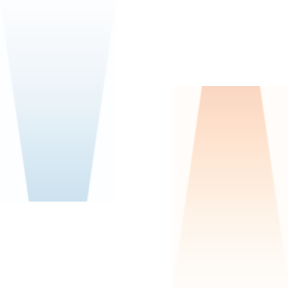
\includegraphics[interpolate=true,width=2.880000in,height=2.880000in]{lpwfa-img0.png}}%
\end{pgfscope}%
\begin{pgfscope}%
\pgfpathrectangle{\pgfqpoint{0.320000in}{0.600000in}}{\pgfqpoint{5.760000in}{2.880000in}}%
\pgfusepath{clip}%
\pgfsetbuttcap%
\pgfsetmiterjoin%
\definecolor{currentfill}{rgb}{0.498039,0.498039,0.498039}%
\pgfsetfillcolor{currentfill}%
\pgfsetlinewidth{0.000000pt}%
\definecolor{currentstroke}{rgb}{0.000000,0.000000,0.000000}%
\pgfsetstrokecolor{currentstroke}%
\pgfsetstrokeopacity{0.000000}%
\pgfsetdash{}{0pt}%
\pgfpathmoveto{\pgfqpoint{0.320000in}{0.600000in}}%
\pgfpathlineto{\pgfqpoint{6.080000in}{0.600000in}}%
\pgfpathlineto{\pgfqpoint{6.080000in}{0.744000in}}%
\pgfpathlineto{\pgfqpoint{3.200000in}{0.744000in}}%
\pgfpathlineto{\pgfqpoint{3.200000in}{1.176000in}}%
\pgfpathlineto{\pgfqpoint{2.624000in}{1.464000in}}%
\pgfpathlineto{\pgfqpoint{2.048000in}{1.464000in}}%
\pgfpathlineto{\pgfqpoint{1.472000in}{1.176000in}}%
\pgfpathlineto{\pgfqpoint{1.472000in}{0.744000in}}%
\pgfpathlineto{\pgfqpoint{0.320000in}{0.744000in}}%
\pgfpathlineto{\pgfqpoint{0.320000in}{0.600000in}}%
\pgfpathclose%
\pgfusepath{fill}%
\end{pgfscope}%
\begin{pgfscope}%
\pgfpathrectangle{\pgfqpoint{0.320000in}{0.600000in}}{\pgfqpoint{5.760000in}{2.880000in}}%
\pgfusepath{clip}%
\pgfsetbuttcap%
\pgfsetmiterjoin%
\definecolor{currentfill}{rgb}{0.498039,0.498039,0.498039}%
\pgfsetfillcolor{currentfill}%
\pgfsetlinewidth{0.000000pt}%
\definecolor{currentstroke}{rgb}{0.000000,0.000000,0.000000}%
\pgfsetstrokecolor{currentstroke}%
\pgfsetstrokeopacity{0.000000}%
\pgfsetdash{}{0pt}%
\pgfpathmoveto{\pgfqpoint{0.320000in}{3.480000in}}%
\pgfpathlineto{\pgfqpoint{6.080000in}{3.480000in}}%
\pgfpathlineto{\pgfqpoint{6.080000in}{3.336000in}}%
\pgfpathlineto{\pgfqpoint{4.928000in}{3.336000in}}%
\pgfpathlineto{\pgfqpoint{4.928000in}{2.904000in}}%
\pgfpathlineto{\pgfqpoint{4.352000in}{2.616000in}}%
\pgfpathlineto{\pgfqpoint{3.776000in}{2.616000in}}%
\pgfpathlineto{\pgfqpoint{3.200000in}{2.904000in}}%
\pgfpathlineto{\pgfqpoint{3.200000in}{3.336000in}}%
\pgfpathlineto{\pgfqpoint{0.320000in}{3.336000in}}%
\pgfpathlineto{\pgfqpoint{0.320000in}{3.480000in}}%
\pgfpathclose%
\pgfusepath{fill}%
\end{pgfscope}%
\begin{pgfscope}%
\pgfpathrectangle{\pgfqpoint{0.320000in}{0.600000in}}{\pgfqpoint{5.760000in}{2.880000in}}%
\pgfusepath{clip}%
\pgfsetbuttcap%
\pgfsetmiterjoin%
\definecolor{currentfill}{rgb}{1.000000,1.000000,1.000000}%
\pgfsetfillcolor{currentfill}%
\pgfsetfillopacity{0.500000}%
\pgfsetlinewidth{1.003750pt}%
\definecolor{currentstroke}{rgb}{0.000000,0.000000,0.000000}%
\pgfsetstrokecolor{currentstroke}%
\pgfsetstrokeopacity{0.500000}%
\pgfsetdash{}{0pt}%
\pgfpathmoveto{\pgfqpoint{2.336000in}{1.896000in}}%
\pgfpathcurveto{\pgfqpoint{2.393284in}{1.896000in}}{\pgfqpoint{2.448229in}{1.911173in}}{\pgfqpoint{2.488735in}{1.938177in}}%
\pgfpathcurveto{\pgfqpoint{2.529241in}{1.965180in}}{\pgfqpoint{2.552000in}{2.001811in}}{\pgfqpoint{2.552000in}{2.040000in}}%
\pgfpathcurveto{\pgfqpoint{2.552000in}{2.078189in}}{\pgfqpoint{2.529241in}{2.114820in}}{\pgfqpoint{2.488735in}{2.141823in}}%
\pgfpathcurveto{\pgfqpoint{2.448229in}{2.168827in}}{\pgfqpoint{2.393284in}{2.184000in}}{\pgfqpoint{2.336000in}{2.184000in}}%
\pgfpathcurveto{\pgfqpoint{2.278716in}{2.184000in}}{\pgfqpoint{2.223771in}{2.168827in}}{\pgfqpoint{2.183265in}{2.141823in}}%
\pgfpathcurveto{\pgfqpoint{2.142759in}{2.114820in}}{\pgfqpoint{2.120000in}{2.078189in}}{\pgfqpoint{2.120000in}{2.040000in}}%
\pgfpathcurveto{\pgfqpoint{2.120000in}{2.001811in}}{\pgfqpoint{2.142759in}{1.965180in}}{\pgfqpoint{2.183265in}{1.938177in}}%
\pgfpathcurveto{\pgfqpoint{2.223771in}{1.911173in}}{\pgfqpoint{2.278716in}{1.896000in}}{\pgfqpoint{2.336000in}{1.896000in}}%
\pgfpathlineto{\pgfqpoint{2.336000in}{1.896000in}}%
\pgfpathclose%
\pgfusepath{stroke,fill}%
\end{pgfscope}%
\begin{pgfscope}%
\pgfpathrectangle{\pgfqpoint{0.320000in}{0.600000in}}{\pgfqpoint{5.760000in}{2.880000in}}%
\pgfusepath{clip}%
\pgfsetbuttcap%
\pgfsetmiterjoin%
\definecolor{currentfill}{rgb}{1.000000,1.000000,1.000000}%
\pgfsetfillcolor{currentfill}%
\pgfsetfillopacity{0.500000}%
\pgfsetlinewidth{1.003750pt}%
\definecolor{currentstroke}{rgb}{0.000000,0.000000,0.000000}%
\pgfsetstrokecolor{currentstroke}%
\pgfsetstrokeopacity{0.500000}%
\pgfsetdash{}{0pt}%
\pgfpathmoveto{\pgfqpoint{4.064000in}{1.896000in}}%
\pgfpathcurveto{\pgfqpoint{4.109827in}{1.896000in}}{\pgfqpoint{4.153783in}{1.911173in}}{\pgfqpoint{4.186188in}{1.938177in}}%
\pgfpathcurveto{\pgfqpoint{4.218593in}{1.965180in}}{\pgfqpoint{4.236800in}{2.001811in}}{\pgfqpoint{4.236800in}{2.040000in}}%
\pgfpathcurveto{\pgfqpoint{4.236800in}{2.078189in}}{\pgfqpoint{4.218593in}{2.114820in}}{\pgfqpoint{4.186188in}{2.141823in}}%
\pgfpathcurveto{\pgfqpoint{4.153783in}{2.168827in}}{\pgfqpoint{4.109827in}{2.184000in}}{\pgfqpoint{4.064000in}{2.184000in}}%
\pgfpathcurveto{\pgfqpoint{4.018173in}{2.184000in}}{\pgfqpoint{3.974217in}{2.168827in}}{\pgfqpoint{3.941812in}{2.141823in}}%
\pgfpathcurveto{\pgfqpoint{3.909407in}{2.114820in}}{\pgfqpoint{3.891200in}{2.078189in}}{\pgfqpoint{3.891200in}{2.040000in}}%
\pgfpathcurveto{\pgfqpoint{3.891200in}{2.001811in}}{\pgfqpoint{3.909407in}{1.965180in}}{\pgfqpoint{3.941812in}{1.938177in}}%
\pgfpathcurveto{\pgfqpoint{3.974217in}{1.911173in}}{\pgfqpoint{4.018173in}{1.896000in}}{\pgfqpoint{4.064000in}{1.896000in}}%
\pgfpathlineto{\pgfqpoint{4.064000in}{1.896000in}}%
\pgfpathclose%
\pgfusepath{stroke,fill}%
\end{pgfscope}%
\begin{pgfscope}%
\pgfpathrectangle{\pgfqpoint{0.320000in}{0.600000in}}{\pgfqpoint{5.760000in}{2.880000in}}%
\pgfusepath{clip}%
\pgfsetbuttcap%
\pgfsetroundjoin%
\definecolor{currentfill}{rgb}{0.839216,0.152941,0.156863}%
\pgfsetfillcolor{currentfill}%
\pgfsetfillopacity{0.300000}%
\pgfsetlinewidth{1.003750pt}%
\definecolor{currentstroke}{rgb}{0.839216,0.152941,0.156863}%
\pgfsetstrokecolor{currentstroke}%
\pgfsetstrokeopacity{0.300000}%
\pgfsetdash{}{0pt}%
\pgfsys@defobject{currentmarker}{\pgfqpoint{-2.560000in}{1.537030in}}{\pgfqpoint{3.200000in}{2.542970in}}{%
\pgfpathmoveto{\pgfqpoint{-2.560000in}{1.537030in}}%
\pgfpathlineto{\pgfqpoint{-2.560000in}{2.542970in}}%
\pgfpathlineto{\pgfqpoint{-2.501818in}{2.537309in}}%
\pgfpathlineto{\pgfqpoint{-2.443636in}{2.531651in}}%
\pgfpathlineto{\pgfqpoint{-2.385455in}{2.525996in}}%
\pgfpathlineto{\pgfqpoint{-2.327273in}{2.520346in}}%
\pgfpathlineto{\pgfqpoint{-2.269091in}{2.514700in}}%
\pgfpathlineto{\pgfqpoint{-2.210909in}{2.509057in}}%
\pgfpathlineto{\pgfqpoint{-2.152727in}{2.503420in}}%
\pgfpathlineto{\pgfqpoint{-2.094545in}{2.497786in}}%
\pgfpathlineto{\pgfqpoint{-2.036364in}{2.492158in}}%
\pgfpathlineto{\pgfqpoint{-1.978182in}{2.486534in}}%
\pgfpathlineto{\pgfqpoint{-1.920000in}{2.480915in}}%
\pgfpathlineto{\pgfqpoint{-1.861818in}{2.475302in}}%
\pgfpathlineto{\pgfqpoint{-1.803636in}{2.469694in}}%
\pgfpathlineto{\pgfqpoint{-1.745455in}{2.464092in}}%
\pgfpathlineto{\pgfqpoint{-1.687273in}{2.458495in}}%
\pgfpathlineto{\pgfqpoint{-1.629091in}{2.452905in}}%
\pgfpathlineto{\pgfqpoint{-1.570909in}{2.447321in}}%
\pgfpathlineto{\pgfqpoint{-1.512727in}{2.441744in}}%
\pgfpathlineto{\pgfqpoint{-1.454545in}{2.436173in}}%
\pgfpathlineto{\pgfqpoint{-1.396364in}{2.430610in}}%
\pgfpathlineto{\pgfqpoint{-1.338182in}{2.425055in}}%
\pgfpathlineto{\pgfqpoint{-1.280000in}{2.419507in}}%
\pgfpathlineto{\pgfqpoint{-1.221818in}{2.413968in}}%
\pgfpathlineto{\pgfqpoint{-1.163636in}{2.408437in}}%
\pgfpathlineto{\pgfqpoint{-1.105455in}{2.402915in}}%
\pgfpathlineto{\pgfqpoint{-1.047273in}{2.397402in}}%
\pgfpathlineto{\pgfqpoint{-0.989091in}{2.391900in}}%
\pgfpathlineto{\pgfqpoint{-0.930909in}{2.386407in}}%
\pgfpathlineto{\pgfqpoint{-0.872727in}{2.380926in}}%
\pgfpathlineto{\pgfqpoint{-0.814545in}{2.375456in}}%
\pgfpathlineto{\pgfqpoint{-0.756364in}{2.369997in}}%
\pgfpathlineto{\pgfqpoint{-0.698182in}{2.364551in}}%
\pgfpathlineto{\pgfqpoint{-0.640000in}{2.359119in}}%
\pgfpathlineto{\pgfqpoint{-0.581818in}{2.353700in}}%
\pgfpathlineto{\pgfqpoint{-0.523636in}{2.348296in}}%
\pgfpathlineto{\pgfqpoint{-0.465455in}{2.342907in}}%
\pgfpathlineto{\pgfqpoint{-0.407273in}{2.337534in}}%
\pgfpathlineto{\pgfqpoint{-0.349091in}{2.332178in}}%
\pgfpathlineto{\pgfqpoint{-0.290909in}{2.326841in}}%
\pgfpathlineto{\pgfqpoint{-0.232727in}{2.321522in}}%
\pgfpathlineto{\pgfqpoint{-0.174545in}{2.316224in}}%
\pgfpathlineto{\pgfqpoint{-0.116364in}{2.310946in}}%
\pgfpathlineto{\pgfqpoint{-0.058182in}{2.305692in}}%
\pgfpathlineto{\pgfqpoint{0.000000in}{2.300461in}}%
\pgfpathlineto{\pgfqpoint{0.058182in}{2.295256in}}%
\pgfpathlineto{\pgfqpoint{0.116364in}{2.290078in}}%
\pgfpathlineto{\pgfqpoint{0.174545in}{2.284928in}}%
\pgfpathlineto{\pgfqpoint{0.232727in}{2.279810in}}%
\pgfpathlineto{\pgfqpoint{0.290909in}{2.274723in}}%
\pgfpathlineto{\pgfqpoint{0.349091in}{2.269672in}}%
\pgfpathlineto{\pgfqpoint{0.407273in}{2.264657in}}%
\pgfpathlineto{\pgfqpoint{0.465455in}{2.259683in}}%
\pgfpathlineto{\pgfqpoint{0.523636in}{2.254750in}}%
\pgfpathlineto{\pgfqpoint{0.581818in}{2.249863in}}%
\pgfpathlineto{\pgfqpoint{0.640000in}{2.245025in}}%
\pgfpathlineto{\pgfqpoint{0.698182in}{2.240239in}}%
\pgfpathlineto{\pgfqpoint{0.756364in}{2.235508in}}%
\pgfpathlineto{\pgfqpoint{0.814545in}{2.230838in}}%
\pgfpathlineto{\pgfqpoint{0.872727in}{2.226233in}}%
\pgfpathlineto{\pgfqpoint{0.930909in}{2.221697in}}%
\pgfpathlineto{\pgfqpoint{0.989091in}{2.217236in}}%
\pgfpathlineto{\pgfqpoint{1.047273in}{2.212856in}}%
\pgfpathlineto{\pgfqpoint{1.105455in}{2.208563in}}%
\pgfpathlineto{\pgfqpoint{1.163636in}{2.204364in}}%
\pgfpathlineto{\pgfqpoint{1.221818in}{2.200266in}}%
\pgfpathlineto{\pgfqpoint{1.280000in}{2.196277in}}%
\pgfpathlineto{\pgfqpoint{1.338182in}{2.192406in}}%
\pgfpathlineto{\pgfqpoint{1.396364in}{2.188661in}}%
\pgfpathlineto{\pgfqpoint{1.454545in}{2.185054in}}%
\pgfpathlineto{\pgfqpoint{1.512727in}{2.181594in}}%
\pgfpathlineto{\pgfqpoint{1.570909in}{2.178292in}}%
\pgfpathlineto{\pgfqpoint{1.629091in}{2.175160in}}%
\pgfpathlineto{\pgfqpoint{1.687273in}{2.172210in}}%
\pgfpathlineto{\pgfqpoint{1.745455in}{2.169455in}}%
\pgfpathlineto{\pgfqpoint{1.803636in}{2.166906in}}%
\pgfpathlineto{\pgfqpoint{1.861818in}{2.164577in}}%
\pgfpathlineto{\pgfqpoint{1.920000in}{2.162481in}}%
\pgfpathlineto{\pgfqpoint{1.978182in}{2.160629in}}%
\pgfpathlineto{\pgfqpoint{2.036364in}{2.159033in}}%
\pgfpathlineto{\pgfqpoint{2.094545in}{2.157703in}}%
\pgfpathlineto{\pgfqpoint{2.152727in}{2.156649in}}%
\pgfpathlineto{\pgfqpoint{2.210909in}{2.155877in}}%
\pgfpathlineto{\pgfqpoint{2.269091in}{2.155394in}}%
\pgfpathlineto{\pgfqpoint{2.327273in}{2.155203in}}%
\pgfpathlineto{\pgfqpoint{2.385455in}{2.155306in}}%
\pgfpathlineto{\pgfqpoint{2.443636in}{2.155702in}}%
\pgfpathlineto{\pgfqpoint{2.501818in}{2.156387in}}%
\pgfpathlineto{\pgfqpoint{2.560000in}{2.157358in}}%
\pgfpathlineto{\pgfqpoint{2.618182in}{2.158606in}}%
\pgfpathlineto{\pgfqpoint{2.676364in}{2.160123in}}%
\pgfpathlineto{\pgfqpoint{2.734545in}{2.161899in}}%
\pgfpathlineto{\pgfqpoint{2.792727in}{2.163924in}}%
\pgfpathlineto{\pgfqpoint{2.850909in}{2.166184in}}%
\pgfpathlineto{\pgfqpoint{2.909091in}{2.168668in}}%
\pgfpathlineto{\pgfqpoint{2.967273in}{2.171362in}}%
\pgfpathlineto{\pgfqpoint{3.025455in}{2.174255in}}%
\pgfpathlineto{\pgfqpoint{3.083636in}{2.177334in}}%
\pgfpathlineto{\pgfqpoint{3.141818in}{2.180586in}}%
\pgfpathlineto{\pgfqpoint{3.200000in}{2.184000in}}%
\pgfpathlineto{\pgfqpoint{3.200000in}{1.896000in}}%
\pgfpathlineto{\pgfqpoint{3.200000in}{1.896000in}}%
\pgfpathlineto{\pgfqpoint{3.141818in}{1.899414in}}%
\pgfpathlineto{\pgfqpoint{3.083636in}{1.902666in}}%
\pgfpathlineto{\pgfqpoint{3.025455in}{1.905745in}}%
\pgfpathlineto{\pgfqpoint{2.967273in}{1.908638in}}%
\pgfpathlineto{\pgfqpoint{2.909091in}{1.911332in}}%
\pgfpathlineto{\pgfqpoint{2.850909in}{1.913816in}}%
\pgfpathlineto{\pgfqpoint{2.792727in}{1.916076in}}%
\pgfpathlineto{\pgfqpoint{2.734545in}{1.918101in}}%
\pgfpathlineto{\pgfqpoint{2.676364in}{1.919877in}}%
\pgfpathlineto{\pgfqpoint{2.618182in}{1.921394in}}%
\pgfpathlineto{\pgfqpoint{2.560000in}{1.922642in}}%
\pgfpathlineto{\pgfqpoint{2.501818in}{1.923613in}}%
\pgfpathlineto{\pgfqpoint{2.443636in}{1.924298in}}%
\pgfpathlineto{\pgfqpoint{2.385455in}{1.924694in}}%
\pgfpathlineto{\pgfqpoint{2.327273in}{1.924797in}}%
\pgfpathlineto{\pgfqpoint{2.269091in}{1.924606in}}%
\pgfpathlineto{\pgfqpoint{2.210909in}{1.924123in}}%
\pgfpathlineto{\pgfqpoint{2.152727in}{1.923351in}}%
\pgfpathlineto{\pgfqpoint{2.094545in}{1.922297in}}%
\pgfpathlineto{\pgfqpoint{2.036364in}{1.920967in}}%
\pgfpathlineto{\pgfqpoint{1.978182in}{1.919371in}}%
\pgfpathlineto{\pgfqpoint{1.920000in}{1.917519in}}%
\pgfpathlineto{\pgfqpoint{1.861818in}{1.915423in}}%
\pgfpathlineto{\pgfqpoint{1.803636in}{1.913094in}}%
\pgfpathlineto{\pgfqpoint{1.745455in}{1.910545in}}%
\pgfpathlineto{\pgfqpoint{1.687273in}{1.907790in}}%
\pgfpathlineto{\pgfqpoint{1.629091in}{1.904840in}}%
\pgfpathlineto{\pgfqpoint{1.570909in}{1.901708in}}%
\pgfpathlineto{\pgfqpoint{1.512727in}{1.898406in}}%
\pgfpathlineto{\pgfqpoint{1.454545in}{1.894946in}}%
\pgfpathlineto{\pgfqpoint{1.396364in}{1.891339in}}%
\pgfpathlineto{\pgfqpoint{1.338182in}{1.887594in}}%
\pgfpathlineto{\pgfqpoint{1.280000in}{1.883723in}}%
\pgfpathlineto{\pgfqpoint{1.221818in}{1.879734in}}%
\pgfpathlineto{\pgfqpoint{1.163636in}{1.875636in}}%
\pgfpathlineto{\pgfqpoint{1.105455in}{1.871437in}}%
\pgfpathlineto{\pgfqpoint{1.047273in}{1.867144in}}%
\pgfpathlineto{\pgfqpoint{0.989091in}{1.862764in}}%
\pgfpathlineto{\pgfqpoint{0.930909in}{1.858303in}}%
\pgfpathlineto{\pgfqpoint{0.872727in}{1.853767in}}%
\pgfpathlineto{\pgfqpoint{0.814545in}{1.849162in}}%
\pgfpathlineto{\pgfqpoint{0.756364in}{1.844492in}}%
\pgfpathlineto{\pgfqpoint{0.698182in}{1.839761in}}%
\pgfpathlineto{\pgfqpoint{0.640000in}{1.834975in}}%
\pgfpathlineto{\pgfqpoint{0.581818in}{1.830137in}}%
\pgfpathlineto{\pgfqpoint{0.523636in}{1.825250in}}%
\pgfpathlineto{\pgfqpoint{0.465455in}{1.820317in}}%
\pgfpathlineto{\pgfqpoint{0.407273in}{1.815343in}}%
\pgfpathlineto{\pgfqpoint{0.349091in}{1.810328in}}%
\pgfpathlineto{\pgfqpoint{0.290909in}{1.805277in}}%
\pgfpathlineto{\pgfqpoint{0.232727in}{1.800190in}}%
\pgfpathlineto{\pgfqpoint{0.174545in}{1.795072in}}%
\pgfpathlineto{\pgfqpoint{0.116364in}{1.789922in}}%
\pgfpathlineto{\pgfqpoint{0.058182in}{1.784744in}}%
\pgfpathlineto{\pgfqpoint{0.000000in}{1.779539in}}%
\pgfpathlineto{\pgfqpoint{-0.058182in}{1.774308in}}%
\pgfpathlineto{\pgfqpoint{-0.116364in}{1.769054in}}%
\pgfpathlineto{\pgfqpoint{-0.174545in}{1.763776in}}%
\pgfpathlineto{\pgfqpoint{-0.232727in}{1.758478in}}%
\pgfpathlineto{\pgfqpoint{-0.290909in}{1.753159in}}%
\pgfpathlineto{\pgfqpoint{-0.349091in}{1.747822in}}%
\pgfpathlineto{\pgfqpoint{-0.407273in}{1.742466in}}%
\pgfpathlineto{\pgfqpoint{-0.465455in}{1.737093in}}%
\pgfpathlineto{\pgfqpoint{-0.523636in}{1.731704in}}%
\pgfpathlineto{\pgfqpoint{-0.581818in}{1.726300in}}%
\pgfpathlineto{\pgfqpoint{-0.640000in}{1.720881in}}%
\pgfpathlineto{\pgfqpoint{-0.698182in}{1.715449in}}%
\pgfpathlineto{\pgfqpoint{-0.756364in}{1.710003in}}%
\pgfpathlineto{\pgfqpoint{-0.814545in}{1.704544in}}%
\pgfpathlineto{\pgfqpoint{-0.872727in}{1.699074in}}%
\pgfpathlineto{\pgfqpoint{-0.930909in}{1.693593in}}%
\pgfpathlineto{\pgfqpoint{-0.989091in}{1.688100in}}%
\pgfpathlineto{\pgfqpoint{-1.047273in}{1.682598in}}%
\pgfpathlineto{\pgfqpoint{-1.105455in}{1.677085in}}%
\pgfpathlineto{\pgfqpoint{-1.163636in}{1.671563in}}%
\pgfpathlineto{\pgfqpoint{-1.221818in}{1.666032in}}%
\pgfpathlineto{\pgfqpoint{-1.280000in}{1.660493in}}%
\pgfpathlineto{\pgfqpoint{-1.338182in}{1.654945in}}%
\pgfpathlineto{\pgfqpoint{-1.396364in}{1.649390in}}%
\pgfpathlineto{\pgfqpoint{-1.454545in}{1.643827in}}%
\pgfpathlineto{\pgfqpoint{-1.512727in}{1.638256in}}%
\pgfpathlineto{\pgfqpoint{-1.570909in}{1.632679in}}%
\pgfpathlineto{\pgfqpoint{-1.629091in}{1.627095in}}%
\pgfpathlineto{\pgfqpoint{-1.687273in}{1.621505in}}%
\pgfpathlineto{\pgfqpoint{-1.745455in}{1.615908in}}%
\pgfpathlineto{\pgfqpoint{-1.803636in}{1.610306in}}%
\pgfpathlineto{\pgfqpoint{-1.861818in}{1.604698in}}%
\pgfpathlineto{\pgfqpoint{-1.920000in}{1.599085in}}%
\pgfpathlineto{\pgfqpoint{-1.978182in}{1.593466in}}%
\pgfpathlineto{\pgfqpoint{-2.036364in}{1.587842in}}%
\pgfpathlineto{\pgfqpoint{-2.094545in}{1.582214in}}%
\pgfpathlineto{\pgfqpoint{-2.152727in}{1.576580in}}%
\pgfpathlineto{\pgfqpoint{-2.210909in}{1.570943in}}%
\pgfpathlineto{\pgfqpoint{-2.269091in}{1.565300in}}%
\pgfpathlineto{\pgfqpoint{-2.327273in}{1.559654in}}%
\pgfpathlineto{\pgfqpoint{-2.385455in}{1.554004in}}%
\pgfpathlineto{\pgfqpoint{-2.443636in}{1.548349in}}%
\pgfpathlineto{\pgfqpoint{-2.501818in}{1.542691in}}%
\pgfpathlineto{\pgfqpoint{-2.560000in}{1.537030in}}%
\pgfpathlineto{\pgfqpoint{-2.560000in}{1.537030in}}%
\pgfpathclose%
\pgfusepath{stroke,fill}%
}%
\begin{pgfscope}%
\pgfsys@transformshift{0.000000in}{0.000000in}%
\pgfsys@useobject{currentmarker}{}%
\end{pgfscope}%
\end{pgfscope}%
\begin{pgfscope}%
\pgfpathrectangle{\pgfqpoint{0.320000in}{0.600000in}}{\pgfqpoint{5.760000in}{2.880000in}}%
\pgfusepath{clip}%
\pgfsetbuttcap%
\pgfsetroundjoin%
\pgfsetlinewidth{1.505625pt}%
\definecolor{currentstroke}{rgb}{0.000000,0.000000,0.000000}%
\pgfsetstrokecolor{currentstroke}%
\pgfsetdash{{1.500000pt}{2.475000pt}}{0.000000pt}%
\pgfpathmoveto{\pgfqpoint{0.310000in}{2.040000in}}%
\pgfpathlineto{\pgfqpoint{6.090000in}{2.040000in}}%
\pgfusepath{stroke}%
\end{pgfscope}%
\begin{pgfscope}%
\pgfpathrectangle{\pgfqpoint{0.320000in}{0.600000in}}{\pgfqpoint{5.760000in}{2.880000in}}%
\pgfusepath{clip}%
\pgfsetrectcap%
\pgfsetroundjoin%
\pgfsetlinewidth{0.501875pt}%
\definecolor{currentstroke}{rgb}{0.839216,0.152941,0.156863}%
\pgfsetstrokecolor{currentstroke}%
\pgfsetdash{}{0pt}%
\pgfpathmoveto{\pgfqpoint{0.348800in}{2.038542in}}%
\pgfpathlineto{\pgfqpoint{0.351984in}{2.039352in}}%
\pgfpathlineto{\pgfqpoint{0.356760in}{2.042651in}}%
\pgfpathlineto{\pgfqpoint{0.359944in}{2.041483in}}%
\pgfpathlineto{\pgfqpoint{0.364720in}{2.035412in}}%
\pgfpathlineto{\pgfqpoint{0.366312in}{2.035195in}}%
\pgfpathlineto{\pgfqpoint{0.367904in}{2.036911in}}%
\pgfpathlineto{\pgfqpoint{0.374271in}{2.048382in}}%
\pgfpathlineto{\pgfqpoint{0.375863in}{2.045963in}}%
\pgfpathlineto{\pgfqpoint{0.382231in}{2.026089in}}%
\pgfpathlineto{\pgfqpoint{0.383823in}{2.029227in}}%
\pgfpathlineto{\pgfqpoint{0.390191in}{2.061980in}}%
\pgfpathlineto{\pgfqpoint{0.391783in}{2.058325in}}%
\pgfpathlineto{\pgfqpoint{0.394967in}{2.030379in}}%
\pgfpathlineto{\pgfqpoint{0.398151in}{2.006926in}}%
\pgfpathlineto{\pgfqpoint{0.399743in}{2.010538in}}%
\pgfpathlineto{\pgfqpoint{0.402927in}{2.050026in}}%
\pgfpathlineto{\pgfqpoint{0.406111in}{2.087399in}}%
\pgfpathlineto{\pgfqpoint{0.407703in}{2.084891in}}%
\pgfpathlineto{\pgfqpoint{0.410886in}{2.031741in}}%
\pgfpathlineto{\pgfqpoint{0.414070in}{1.975310in}}%
\pgfpathlineto{\pgfqpoint{0.415662in}{1.975059in}}%
\pgfpathlineto{\pgfqpoint{0.417254in}{1.999818in}}%
\pgfpathlineto{\pgfqpoint{0.422030in}{2.124047in}}%
\pgfpathlineto{\pgfqpoint{0.423622in}{2.129312in}}%
\pgfpathlineto{\pgfqpoint{0.425214in}{2.101066in}}%
\pgfpathlineto{\pgfqpoint{0.429990in}{1.936117in}}%
\pgfpathlineto{\pgfqpoint{0.431582in}{1.923126in}}%
\pgfpathlineto{\pgfqpoint{0.433174in}{1.953100in}}%
\pgfpathlineto{\pgfqpoint{0.439542in}{2.185609in}}%
\pgfpathlineto{\pgfqpoint{0.441134in}{2.156471in}}%
\pgfpathlineto{\pgfqpoint{0.447502in}{1.867235in}}%
\pgfpathlineto{\pgfqpoint{0.449093in}{1.892415in}}%
\pgfpathlineto{\pgfqpoint{0.455461in}{2.235233in}}%
\pgfpathlineto{\pgfqpoint{0.457053in}{2.217258in}}%
\pgfpathlineto{\pgfqpoint{0.460237in}{2.012093in}}%
\pgfpathlineto{\pgfqpoint{0.463421in}{1.829904in}}%
\pgfpathlineto{\pgfqpoint{0.465013in}{1.837840in}}%
\pgfpathlineto{\pgfqpoint{0.468197in}{2.047049in}}%
\pgfpathlineto{\pgfqpoint{0.471381in}{2.255219in}}%
\pgfpathlineto{\pgfqpoint{0.472973in}{2.259205in}}%
\pgfpathlineto{\pgfqpoint{0.474565in}{2.184025in}}%
\pgfpathlineto{\pgfqpoint{0.479341in}{1.830271in}}%
\pgfpathlineto{\pgfqpoint{0.480933in}{1.813824in}}%
\pgfpathlineto{\pgfqpoint{0.482525in}{1.878557in}}%
\pgfpathlineto{\pgfqpoint{0.487301in}{2.234230in}}%
\pgfpathlineto{\pgfqpoint{0.488892in}{2.262186in}}%
\pgfpathlineto{\pgfqpoint{0.490484in}{2.210501in}}%
\pgfpathlineto{\pgfqpoint{0.496852in}{1.832130in}}%
\pgfpathlineto{\pgfqpoint{0.498444in}{1.869721in}}%
\pgfpathlineto{\pgfqpoint{0.504812in}{2.225223in}}%
\pgfpathlineto{\pgfqpoint{0.506404in}{2.201216in}}%
\pgfpathlineto{\pgfqpoint{0.512772in}{1.882835in}}%
\pgfpathlineto{\pgfqpoint{0.514364in}{1.895046in}}%
\pgfpathlineto{\pgfqpoint{0.520732in}{2.166940in}}%
\pgfpathlineto{\pgfqpoint{0.522324in}{2.163923in}}%
\pgfpathlineto{\pgfqpoint{0.525508in}{2.049307in}}%
\pgfpathlineto{\pgfqpoint{0.528691in}{1.942473in}}%
\pgfpathlineto{\pgfqpoint{0.530283in}{1.939183in}}%
\pgfpathlineto{\pgfqpoint{0.533467in}{2.023322in}}%
\pgfpathlineto{\pgfqpoint{0.536651in}{2.111202in}}%
\pgfpathlineto{\pgfqpoint{0.538243in}{2.118092in}}%
\pgfpathlineto{\pgfqpoint{0.539835in}{2.097488in}}%
\pgfpathlineto{\pgfqpoint{0.544611in}{1.990676in}}%
\pgfpathlineto{\pgfqpoint{0.546203in}{1.982392in}}%
\pgfpathlineto{\pgfqpoint{0.547795in}{1.994749in}}%
\pgfpathlineto{\pgfqpoint{0.552571in}{2.072352in}}%
\pgfpathlineto{\pgfqpoint{0.554163in}{2.080476in}}%
\pgfpathlineto{\pgfqpoint{0.555755in}{2.073773in}}%
\pgfpathlineto{\pgfqpoint{0.562123in}{2.012920in}}%
\pgfpathlineto{\pgfqpoint{0.563715in}{2.016060in}}%
\pgfpathlineto{\pgfqpoint{0.570082in}{2.057245in}}%
\pgfpathlineto{\pgfqpoint{0.571674in}{2.056136in}}%
\pgfpathlineto{\pgfqpoint{0.578042in}{2.029554in}}%
\pgfpathlineto{\pgfqpoint{0.579634in}{2.029649in}}%
\pgfpathlineto{\pgfqpoint{0.582818in}{2.038378in}}%
\pgfpathlineto{\pgfqpoint{0.586002in}{2.046012in}}%
\pgfpathlineto{\pgfqpoint{0.587594in}{2.046322in}}%
\pgfpathlineto{\pgfqpoint{0.590778in}{2.041475in}}%
\pgfpathlineto{\pgfqpoint{0.593962in}{2.036717in}}%
\pgfpathlineto{\pgfqpoint{0.595554in}{2.036323in}}%
\pgfpathlineto{\pgfqpoint{0.598738in}{2.038873in}}%
\pgfpathlineto{\pgfqpoint{0.601922in}{2.041697in}}%
\pgfpathlineto{\pgfqpoint{0.605106in}{2.041630in}}%
\pgfpathlineto{\pgfqpoint{0.611473in}{2.038925in}}%
\pgfpathlineto{\pgfqpoint{0.632169in}{2.039964in}}%
\pgfpathlineto{\pgfqpoint{0.649680in}{2.040007in}}%
\pgfpathlineto{\pgfqpoint{0.665600in}{2.040000in}}%
\pgfpathlineto{\pgfqpoint{0.665600in}{2.040000in}}%
\pgfusepath{stroke}%
\end{pgfscope}%
\begin{pgfscope}%
\pgfpathrectangle{\pgfqpoint{0.320000in}{0.600000in}}{\pgfqpoint{5.760000in}{2.880000in}}%
\pgfusepath{clip}%
\pgfsetrectcap%
\pgfsetroundjoin%
\pgfsetlinewidth{0.501875pt}%
\definecolor{currentstroke}{rgb}{0.839216,0.152941,0.156863}%
\pgfsetstrokecolor{currentstroke}%
\pgfsetdash{}{0pt}%
\pgfpathmoveto{\pgfqpoint{2.336000in}{2.040000in}}%
\pgfpathlineto{\pgfqpoint{2.339256in}{2.026860in}}%
\pgfpathlineto{\pgfqpoint{2.340342in}{2.025558in}}%
\pgfpathlineto{\pgfqpoint{2.341427in}{2.026725in}}%
\pgfpathlineto{\pgfqpoint{2.343598in}{2.036071in}}%
\pgfpathlineto{\pgfqpoint{2.347940in}{2.059197in}}%
\pgfpathlineto{\pgfqpoint{2.349025in}{2.059538in}}%
\pgfpathlineto{\pgfqpoint{2.351196in}{2.050130in}}%
\pgfpathlineto{\pgfqpoint{2.356623in}{2.013590in}}%
\pgfpathlineto{\pgfqpoint{2.357709in}{2.015148in}}%
\pgfpathlineto{\pgfqpoint{2.359879in}{2.031086in}}%
\pgfpathlineto{\pgfqpoint{2.364221in}{2.072927in}}%
\pgfpathlineto{\pgfqpoint{2.365307in}{2.074236in}}%
\pgfpathlineto{\pgfqpoint{2.366392in}{2.069591in}}%
\pgfpathlineto{\pgfqpoint{2.369648in}{2.029032in}}%
\pgfpathlineto{\pgfqpoint{2.372905in}{1.996598in}}%
\pgfpathlineto{\pgfqpoint{2.373990in}{1.998227in}}%
\pgfpathlineto{\pgfqpoint{2.376161in}{2.022636in}}%
\pgfpathlineto{\pgfqpoint{2.380503in}{2.090745in}}%
\pgfpathlineto{\pgfqpoint{2.381588in}{2.093908in}}%
\pgfpathlineto{\pgfqpoint{2.382673in}{2.087811in}}%
\pgfpathlineto{\pgfqpoint{2.384844in}{2.051726in}}%
\pgfpathlineto{\pgfqpoint{2.389186in}{1.975895in}}%
\pgfpathlineto{\pgfqpoint{2.390271in}{1.976937in}}%
\pgfpathlineto{\pgfqpoint{2.392442in}{2.010489in}}%
\pgfpathlineto{\pgfqpoint{2.396784in}{2.110257in}}%
\pgfpathlineto{\pgfqpoint{2.397869in}{2.116280in}}%
\pgfpathlineto{\pgfqpoint{2.398955in}{2.109314in}}%
\pgfpathlineto{\pgfqpoint{2.401126in}{2.061428in}}%
\pgfpathlineto{\pgfqpoint{2.405467in}{1.954912in}}%
\pgfpathlineto{\pgfqpoint{2.406553in}{1.954475in}}%
\pgfpathlineto{\pgfqpoint{2.408724in}{1.995833in}}%
\pgfpathlineto{\pgfqpoint{2.414151in}{2.137006in}}%
\pgfpathlineto{\pgfqpoint{2.415236in}{2.130203in}}%
\pgfpathlineto{\pgfqpoint{2.417407in}{2.073089in}}%
\pgfpathlineto{\pgfqpoint{2.421749in}{1.938514in}}%
\pgfpathlineto{\pgfqpoint{2.422834in}{1.935786in}}%
\pgfpathlineto{\pgfqpoint{2.423920in}{1.950860in}}%
\pgfpathlineto{\pgfqpoint{2.427176in}{2.067260in}}%
\pgfpathlineto{\pgfqpoint{2.430432in}{2.150869in}}%
\pgfpathlineto{\pgfqpoint{2.431518in}{2.145411in}}%
\pgfpathlineto{\pgfqpoint{2.433688in}{2.084217in}}%
\pgfpathlineto{\pgfqpoint{2.438030in}{1.931245in}}%
\pgfpathlineto{\pgfqpoint{2.439116in}{1.925887in}}%
\pgfpathlineto{\pgfqpoint{2.440201in}{1.939912in}}%
\pgfpathlineto{\pgfqpoint{2.443457in}{2.061246in}}%
\pgfpathlineto{\pgfqpoint{2.446714in}{2.153877in}}%
\pgfpathlineto{\pgfqpoint{2.447799in}{2.150646in}}%
\pgfpathlineto{\pgfqpoint{2.449970in}{2.091780in}}%
\pgfpathlineto{\pgfqpoint{2.454312in}{1.935309in}}%
\pgfpathlineto{\pgfqpoint{2.455397in}{1.927707in}}%
\pgfpathlineto{\pgfqpoint{2.456482in}{1.939145in}}%
\pgfpathlineto{\pgfqpoint{2.459739in}{2.052973in}}%
\pgfpathlineto{\pgfqpoint{2.462995in}{2.145112in}}%
\pgfpathlineto{\pgfqpoint{2.464080in}{2.144342in}}%
\pgfpathlineto{\pgfqpoint{2.466251in}{2.093542in}}%
\pgfpathlineto{\pgfqpoint{2.470593in}{1.949493in}}%
\pgfpathlineto{\pgfqpoint{2.471678in}{1.940689in}}%
\pgfpathlineto{\pgfqpoint{2.472764in}{1.948759in}}%
\pgfpathlineto{\pgfqpoint{2.474935in}{2.005981in}}%
\pgfpathlineto{\pgfqpoint{2.479276in}{2.127179in}}%
\pgfpathlineto{\pgfqpoint{2.480362in}{2.128416in}}%
\pgfpathlineto{\pgfqpoint{2.482533in}{2.089121in}}%
\pgfpathlineto{\pgfqpoint{2.486874in}{1.969754in}}%
\pgfpathlineto{\pgfqpoint{2.487960in}{1.961065in}}%
\pgfpathlineto{\pgfqpoint{2.489045in}{1.965868in}}%
\pgfpathlineto{\pgfqpoint{2.491216in}{2.008749in}}%
\pgfpathlineto{\pgfqpoint{2.495558in}{2.104959in}}%
\pgfpathlineto{\pgfqpoint{2.496643in}{2.107327in}}%
\pgfpathlineto{\pgfqpoint{2.497729in}{2.098384in}}%
\pgfpathlineto{\pgfqpoint{2.504241in}{1.983617in}}%
\pgfpathlineto{\pgfqpoint{2.505327in}{1.985895in}}%
\pgfpathlineto{\pgfqpoint{2.507497in}{2.014752in}}%
\pgfpathlineto{\pgfqpoint{2.511839in}{2.083475in}}%
\pgfpathlineto{\pgfqpoint{2.512925in}{2.086075in}}%
\pgfpathlineto{\pgfqpoint{2.514010in}{2.080894in}}%
\pgfpathlineto{\pgfqpoint{2.517266in}{2.036292in}}%
\pgfpathlineto{\pgfqpoint{2.520523in}{2.003810in}}%
\pgfpathlineto{\pgfqpoint{2.521608in}{2.004520in}}%
\pgfpathlineto{\pgfqpoint{2.523779in}{2.021948in}}%
\pgfpathlineto{\pgfqpoint{2.528121in}{2.066128in}}%
\pgfpathlineto{\pgfqpoint{2.529206in}{2.068338in}}%
\pgfpathlineto{\pgfqpoint{2.530291in}{2.065720in}}%
\pgfpathlineto{\pgfqpoint{2.533548in}{2.039419in}}%
\pgfpathlineto{\pgfqpoint{2.536804in}{2.019128in}}%
\pgfpathlineto{\pgfqpoint{2.537889in}{2.019093in}}%
\pgfpathlineto{\pgfqpoint{2.540060in}{2.028532in}}%
\pgfpathlineto{\pgfqpoint{2.544402in}{2.054095in}}%
\pgfpathlineto{\pgfqpoint{2.545487in}{2.055664in}}%
\pgfpathlineto{\pgfqpoint{2.546573in}{2.054530in}}%
\pgfpathlineto{\pgfqpoint{2.549829in}{2.040576in}}%
\pgfpathlineto{\pgfqpoint{2.552000in}{2.031414in}}%
\pgfpathlineto{\pgfqpoint{2.552000in}{2.031414in}}%
\pgfusepath{stroke}%
\end{pgfscope}%
\begin{pgfscope}%
\pgfpathrectangle{\pgfqpoint{0.320000in}{0.600000in}}{\pgfqpoint{5.760000in}{2.880000in}}%
\pgfusepath{clip}%
\pgfsetrectcap%
\pgfsetroundjoin%
\pgfsetlinewidth{1.003750pt}%
\definecolor{currentstroke}{rgb}{0.000000,0.000000,0.000000}%
\pgfsetstrokecolor{currentstroke}%
\pgfsetdash{}{0pt}%
\pgfpathmoveto{\pgfqpoint{3.776000in}{2.587200in}}%
\pgfpathlineto{\pgfqpoint{3.776000in}{2.558400in}}%
\pgfusepath{stroke}%
\end{pgfscope}%
\begin{pgfscope}%
\pgfpathrectangle{\pgfqpoint{0.320000in}{0.600000in}}{\pgfqpoint{5.760000in}{2.880000in}}%
\pgfusepath{clip}%
\pgfsetrectcap%
\pgfsetroundjoin%
\pgfsetlinewidth{1.003750pt}%
\definecolor{currentstroke}{rgb}{0.000000,0.000000,0.000000}%
\pgfsetstrokecolor{currentstroke}%
\pgfsetdash{}{0pt}%
\pgfpathmoveto{\pgfqpoint{4.352000in}{2.587200in}}%
\pgfpathlineto{\pgfqpoint{4.352000in}{2.558400in}}%
\pgfusepath{stroke}%
\end{pgfscope}%
\begin{pgfscope}%
\pgfpathrectangle{\pgfqpoint{0.320000in}{0.600000in}}{\pgfqpoint{5.760000in}{2.880000in}}%
\pgfusepath{clip}%
\pgfsetrectcap%
\pgfsetroundjoin%
\pgfsetlinewidth{1.003750pt}%
\definecolor{currentstroke}{rgb}{0.000000,0.000000,0.000000}%
\pgfsetstrokecolor{currentstroke}%
\pgfsetdash{}{0pt}%
\pgfpathmoveto{\pgfqpoint{3.776000in}{2.572800in}}%
\pgfpathlineto{\pgfqpoint{3.862400in}{2.572800in}}%
\pgfusepath{stroke}%
\end{pgfscope}%
\begin{pgfscope}%
\pgfpathrectangle{\pgfqpoint{0.320000in}{0.600000in}}{\pgfqpoint{5.760000in}{2.880000in}}%
\pgfusepath{clip}%
\pgfsetrectcap%
\pgfsetroundjoin%
\pgfsetlinewidth{1.003750pt}%
\definecolor{currentstroke}{rgb}{0.000000,0.000000,0.000000}%
\pgfsetstrokecolor{currentstroke}%
\pgfsetdash{}{0pt}%
\pgfpathmoveto{\pgfqpoint{4.265600in}{2.572800in}}%
\pgfpathlineto{\pgfqpoint{4.352000in}{2.572800in}}%
\pgfusepath{stroke}%
\end{pgfscope}%
\begin{pgfscope}%
\pgfpathrectangle{\pgfqpoint{0.320000in}{0.600000in}}{\pgfqpoint{5.760000in}{2.880000in}}%
\pgfusepath{clip}%
\pgfsetrectcap%
\pgfsetroundjoin%
\pgfsetlinewidth{1.003750pt}%
\definecolor{currentstroke}{rgb}{0.000000,0.000000,0.000000}%
\pgfsetstrokecolor{currentstroke}%
\pgfsetdash{}{0pt}%
\pgfpathmoveto{\pgfqpoint{2.048000in}{1.492800in}}%
\pgfpathlineto{\pgfqpoint{2.048000in}{1.521600in}}%
\pgfusepath{stroke}%
\end{pgfscope}%
\begin{pgfscope}%
\pgfpathrectangle{\pgfqpoint{0.320000in}{0.600000in}}{\pgfqpoint{5.760000in}{2.880000in}}%
\pgfusepath{clip}%
\pgfsetrectcap%
\pgfsetroundjoin%
\pgfsetlinewidth{1.003750pt}%
\definecolor{currentstroke}{rgb}{0.000000,0.000000,0.000000}%
\pgfsetstrokecolor{currentstroke}%
\pgfsetdash{}{0pt}%
\pgfpathmoveto{\pgfqpoint{2.624000in}{1.492800in}}%
\pgfpathlineto{\pgfqpoint{2.624000in}{1.521600in}}%
\pgfusepath{stroke}%
\end{pgfscope}%
\begin{pgfscope}%
\pgfpathrectangle{\pgfqpoint{0.320000in}{0.600000in}}{\pgfqpoint{5.760000in}{2.880000in}}%
\pgfusepath{clip}%
\pgfsetrectcap%
\pgfsetroundjoin%
\pgfsetlinewidth{1.003750pt}%
\definecolor{currentstroke}{rgb}{0.000000,0.000000,0.000000}%
\pgfsetstrokecolor{currentstroke}%
\pgfsetdash{}{0pt}%
\pgfpathmoveto{\pgfqpoint{2.048000in}{1.507200in}}%
\pgfpathlineto{\pgfqpoint{2.134400in}{1.507200in}}%
\pgfusepath{stroke}%
\end{pgfscope}%
\begin{pgfscope}%
\pgfpathrectangle{\pgfqpoint{0.320000in}{0.600000in}}{\pgfqpoint{5.760000in}{2.880000in}}%
\pgfusepath{clip}%
\pgfsetrectcap%
\pgfsetroundjoin%
\pgfsetlinewidth{1.003750pt}%
\definecolor{currentstroke}{rgb}{0.000000,0.000000,0.000000}%
\pgfsetstrokecolor{currentstroke}%
\pgfsetdash{}{0pt}%
\pgfpathmoveto{\pgfqpoint{2.537600in}{1.507200in}}%
\pgfpathlineto{\pgfqpoint{2.624000in}{1.507200in}}%
\pgfusepath{stroke}%
\end{pgfscope}%
\begin{pgfscope}%
\definecolor{textcolor}{rgb}{1.000000,1.000000,1.000000}%
\pgfsetstrokecolor{textcolor}%
\pgfsetfillcolor{textcolor}%
\pgftext[x=2.336000in,y=1.032000in,,base]{\color{textcolor}\sffamily\fontsize{15.000000}{18.000000}\selectfont Gas jet 1}%
\end{pgfscope}%
\begin{pgfscope}%
\definecolor{textcolor}{rgb}{1.000000,1.000000,1.000000}%
\pgfsetstrokecolor{textcolor}%
\pgfsetfillcolor{textcolor}%
\pgftext[x=4.064000in,y=3.048000in,,base]{\color{textcolor}\sffamily\fontsize{15.000000}{18.000000}\selectfont Gas jet 2}%
\end{pgfscope}%
\begin{pgfscope}%
\definecolor{textcolor}{rgb}{0.000000,0.000000,0.000000}%
\pgfsetstrokecolor{textcolor}%
\pgfsetfillcolor{textcolor}%
\pgftext[x=4.064000in,y=2.500800in,,base]{\color{textcolor}\sffamily\fontsize{10.000000}{12.000000}\selectfont \(\displaystyle 3 \, \mathrm{mm}\)}%
\end{pgfscope}%
\begin{pgfscope}%
\definecolor{textcolor}{rgb}{0.000000,0.000000,0.000000}%
\pgfsetstrokecolor{textcolor}%
\pgfsetfillcolor{textcolor}%
\pgftext[x=2.336000in,y=1.478400in,,base]{\color{textcolor}\sffamily\fontsize{10.000000}{12.000000}\selectfont \(\displaystyle 3 \, \mathrm{mm}\)}%
\end{pgfscope}%
\begin{pgfscope}%
\definecolor{textcolor}{rgb}{0.000000,0.000000,0.000000}%
\pgfsetstrokecolor{textcolor}%
\pgfsetfillcolor{textcolor}%
\pgftext[x=2.336000in,y=3.048000in,,base]{\color{textcolor}\sffamily\fontsize{10.000000}{12.000000}\selectfont \textbf{LWFA stage}}%
\end{pgfscope}%
\begin{pgfscope}%
\definecolor{textcolor}{rgb}{0.000000,0.000000,0.000000}%
\pgfsetstrokecolor{textcolor}%
\pgfsetfillcolor{textcolor}%
\pgftext[x=4.064000in,y=1.032000in,,base]{\color{textcolor}\sffamily\fontsize{10.000000}{12.000000}\selectfont \textbf{PWFA stage}}%
\end{pgfscope}%
\begin{pgfscope}%
\definecolor{textcolor}{rgb}{0.000000,0.000000,0.000000}%
\pgfsetstrokecolor{textcolor}%
\pgfsetfillcolor{textcolor}%
\pgftext[x=2.278400in,y=2.385600in,,base]{\color{textcolor}\sffamily\fontsize{10.000000}{12.000000}\selectfont LWFA beam}%
\end{pgfscope}%
\begin{pgfscope}%
\definecolor{textcolor}{rgb}{0.000000,0.000000,0.000000}%
\pgfsetstrokecolor{textcolor}%
\pgfsetfillcolor{textcolor}%
\pgftext[x=4.006400in,y=1.636800in,,base]{\color{textcolor}\sffamily\fontsize{10.000000}{12.000000}\selectfont PWFA beam}%
\end{pgfscope}%
\begin{pgfscope}%
\definecolor{textcolor}{rgb}{0.000000,0.000000,0.000000}%
\pgfsetstrokecolor{textcolor}%
\pgfsetfillcolor{textcolor}%
\pgftext[x=2.736652in, y=2.758747in, left, base]{\color{textcolor}\sffamily\fontsize{10.000000}{12.000000}\selectfont Laser }%
\end{pgfscope}%
\begin{pgfscope}%
\definecolor{textcolor}{rgb}{0.000000,0.000000,0.000000}%
\pgfsetstrokecolor{textcolor}%
\pgfsetfillcolor{textcolor}%
\pgftext[x=2.705402in, y=2.616000in, left, base]{\color{textcolor}\sffamily\fontsize{10.000000}{12.000000}\selectfont  blocker}%
\end{pgfscope}%
\begin{pgfscope}%
\definecolor{textcolor}{rgb}{0.000000,0.000000,0.000000}%
\pgfsetstrokecolor{textcolor}%
\pgfsetfillcolor{textcolor}%
\pgftext[x=0.330570in, y=1.693147in, left, base]{\color{textcolor}\sffamily\fontsize{10.000000}{12.000000}\selectfont drive }%
\end{pgfscope}%
\begin{pgfscope}%
\definecolor{textcolor}{rgb}{0.000000,0.000000,0.000000}%
\pgfsetstrokecolor{textcolor}%
\pgfsetfillcolor{textcolor}%
\pgftext[x=0.361627in, y=1.550400in, left, base]{\color{textcolor}\sffamily\fontsize{10.000000}{12.000000}\selectfont  laser}%
\end{pgfscope}%
\begin{pgfscope}%
\pgfpathrectangle{\pgfqpoint{0.320000in}{0.600000in}}{\pgfqpoint{5.760000in}{2.880000in}}%
\pgfusepath{clip}%
\pgfsetbuttcap%
\pgfsetmiterjoin%
\definecolor{currentfill}{rgb}{0.549020,0.337255,0.294118}%
\pgfsetfillcolor{currentfill}%
\pgfsetlinewidth{1.003750pt}%
\definecolor{currentstroke}{rgb}{0.549020,0.337255,0.294118}%
\pgfsetstrokecolor{currentstroke}%
\pgfsetdash{}{0pt}%
\pgfpathmoveto{\pgfqpoint{3.171200in}{1.608000in}}%
\pgfpathlineto{\pgfqpoint{3.228800in}{1.608000in}}%
\pgfpathlineto{\pgfqpoint{3.228800in}{2.472000in}}%
\pgfpathlineto{\pgfqpoint{3.171200in}{2.472000in}}%
\pgfpathlineto{\pgfqpoint{3.171200in}{1.608000in}}%
\pgfpathclose%
\pgfusepath{stroke,fill}%
\end{pgfscope}%
\begin{pgfscope}%
\pgfpathrectangle{\pgfqpoint{0.320000in}{0.600000in}}{\pgfqpoint{5.760000in}{2.880000in}}%
\pgfusepath{clip}%
\pgfsetbuttcap%
\pgfsetmiterjoin%
\definecolor{currentfill}{rgb}{0.121569,0.466667,0.705882}%
\pgfsetfillcolor{currentfill}%
\pgfsetlinewidth{0.000000pt}%
\definecolor{currentstroke}{rgb}{0.000000,0.000000,0.000000}%
\pgfsetstrokecolor{currentstroke}%
\pgfsetstrokeopacity{0.000000}%
\pgfsetdash{}{0pt}%
\pgfpathmoveto{\pgfqpoint{2.220800in}{1.982400in}}%
\pgfpathcurveto{\pgfqpoint{2.232257in}{1.982400in}}{\pgfqpoint{2.243246in}{1.988469in}}{\pgfqpoint{2.251347in}{1.999271in}}%
\pgfpathcurveto{\pgfqpoint{2.259448in}{2.010072in}}{\pgfqpoint{2.264000in}{2.024724in}}{\pgfqpoint{2.264000in}{2.040000in}}%
\pgfpathcurveto{\pgfqpoint{2.264000in}{2.055276in}}{\pgfqpoint{2.259448in}{2.069928in}}{\pgfqpoint{2.251347in}{2.080729in}}%
\pgfpathcurveto{\pgfqpoint{2.243246in}{2.091531in}}{\pgfqpoint{2.232257in}{2.097600in}}{\pgfqpoint{2.220800in}{2.097600in}}%
\pgfpathcurveto{\pgfqpoint{2.209343in}{2.097600in}}{\pgfqpoint{2.198354in}{2.091531in}}{\pgfqpoint{2.190253in}{2.080729in}}%
\pgfpathcurveto{\pgfqpoint{2.182152in}{2.069928in}}{\pgfqpoint{2.177600in}{2.055276in}}{\pgfqpoint{2.177600in}{2.040000in}}%
\pgfpathcurveto{\pgfqpoint{2.177600in}{2.024724in}}{\pgfqpoint{2.182152in}{2.010072in}}{\pgfqpoint{2.190253in}{1.999271in}}%
\pgfpathcurveto{\pgfqpoint{2.198354in}{1.988469in}}{\pgfqpoint{2.209343in}{1.982400in}}{\pgfqpoint{2.220800in}{1.982400in}}%
\pgfpathlineto{\pgfqpoint{2.220800in}{1.982400in}}%
\pgfpathclose%
\pgfusepath{fill}%
\end{pgfscope}%
\begin{pgfscope}%
\pgfpathrectangle{\pgfqpoint{0.320000in}{0.600000in}}{\pgfqpoint{5.760000in}{2.880000in}}%
\pgfusepath{clip}%
\pgfsetbuttcap%
\pgfsetmiterjoin%
\definecolor{currentfill}{rgb}{0.121569,0.466667,0.705882}%
\pgfsetfillcolor{currentfill}%
\pgfsetlinewidth{0.000000pt}%
\definecolor{currentstroke}{rgb}{0.000000,0.000000,0.000000}%
\pgfsetstrokecolor{currentstroke}%
\pgfsetstrokeopacity{0.000000}%
\pgfsetdash{}{0pt}%
\pgfpathmoveto{\pgfqpoint{4.150400in}{1.953600in}}%
\pgfpathcurveto{\pgfqpoint{4.161857in}{1.953600in}}{\pgfqpoint{4.172846in}{1.962704in}}{\pgfqpoint{4.180947in}{1.978906in}}%
\pgfpathcurveto{\pgfqpoint{4.189048in}{1.995108in}}{\pgfqpoint{4.193600in}{2.017086in}}{\pgfqpoint{4.193600in}{2.040000in}}%
\pgfpathcurveto{\pgfqpoint{4.193600in}{2.062914in}}{\pgfqpoint{4.189048in}{2.084892in}}{\pgfqpoint{4.180947in}{2.101094in}}%
\pgfpathcurveto{\pgfqpoint{4.172846in}{2.117296in}}{\pgfqpoint{4.161857in}{2.126400in}}{\pgfqpoint{4.150400in}{2.126400in}}%
\pgfpathcurveto{\pgfqpoint{4.138943in}{2.126400in}}{\pgfqpoint{4.127954in}{2.117296in}}{\pgfqpoint{4.119853in}{2.101094in}}%
\pgfpathcurveto{\pgfqpoint{4.111752in}{2.084892in}}{\pgfqpoint{4.107200in}{2.062914in}}{\pgfqpoint{4.107200in}{2.040000in}}%
\pgfpathcurveto{\pgfqpoint{4.107200in}{2.017086in}}{\pgfqpoint{4.111752in}{1.995108in}}{\pgfqpoint{4.119853in}{1.978906in}}%
\pgfpathcurveto{\pgfqpoint{4.127954in}{1.962704in}}{\pgfqpoint{4.138943in}{1.953600in}}{\pgfqpoint{4.150400in}{1.953600in}}%
\pgfpathlineto{\pgfqpoint{4.150400in}{1.953600in}}%
\pgfpathclose%
\pgfusepath{fill}%
\end{pgfscope}%
\begin{pgfscope}%
\pgfpathrectangle{\pgfqpoint{0.320000in}{0.600000in}}{\pgfqpoint{5.760000in}{2.880000in}}%
\pgfusepath{clip}%
\pgfsetbuttcap%
\pgfsetmiterjoin%
\definecolor{currentfill}{rgb}{1.000000,0.498039,0.054902}%
\pgfsetfillcolor{currentfill}%
\pgfsetlinewidth{0.000000pt}%
\definecolor{currentstroke}{rgb}{0.000000,0.000000,0.000000}%
\pgfsetstrokecolor{currentstroke}%
\pgfsetstrokeopacity{0.000000}%
\pgfsetdash{}{0pt}%
\pgfpathmoveto{\pgfqpoint{3.948800in}{1.982400in}}%
\pgfpathcurveto{\pgfqpoint{3.956438in}{1.982400in}}{\pgfqpoint{3.963764in}{1.988469in}}{\pgfqpoint{3.969165in}{1.999271in}}%
\pgfpathcurveto{\pgfqpoint{3.974565in}{2.010072in}}{\pgfqpoint{3.977600in}{2.024724in}}{\pgfqpoint{3.977600in}{2.040000in}}%
\pgfpathcurveto{\pgfqpoint{3.977600in}{2.055276in}}{\pgfqpoint{3.974565in}{2.069928in}}{\pgfqpoint{3.969165in}{2.080729in}}%
\pgfpathcurveto{\pgfqpoint{3.963764in}{2.091531in}}{\pgfqpoint{3.956438in}{2.097600in}}{\pgfqpoint{3.948800in}{2.097600in}}%
\pgfpathcurveto{\pgfqpoint{3.941162in}{2.097600in}}{\pgfqpoint{3.933836in}{2.091531in}}{\pgfqpoint{3.928435in}{2.080729in}}%
\pgfpathcurveto{\pgfqpoint{3.923035in}{2.069928in}}{\pgfqpoint{3.920000in}{2.055276in}}{\pgfqpoint{3.920000in}{2.040000in}}%
\pgfpathcurveto{\pgfqpoint{3.920000in}{2.024724in}}{\pgfqpoint{3.923035in}{2.010072in}}{\pgfqpoint{3.928435in}{1.999271in}}%
\pgfpathcurveto{\pgfqpoint{3.933836in}{1.988469in}}{\pgfqpoint{3.941162in}{1.982400in}}{\pgfqpoint{3.948800in}{1.982400in}}%
\pgfpathlineto{\pgfqpoint{3.948800in}{1.982400in}}%
\pgfpathclose%
\pgfusepath{fill}%
\end{pgfscope}%
\begin{pgfscope}%
\pgfpathrectangle{\pgfqpoint{0.320000in}{0.600000in}}{\pgfqpoint{5.760000in}{2.880000in}}%
\pgfusepath{clip}%
\pgfsetbuttcap%
\pgfsetmiterjoin%
\definecolor{currentfill}{rgb}{0.000000,0.000000,0.000000}%
\pgfsetfillcolor{currentfill}%
\pgfsetlinewidth{0.000000pt}%
\definecolor{currentstroke}{rgb}{0.000000,0.000000,0.000000}%
\pgfsetstrokecolor{currentstroke}%
\pgfsetstrokeopacity{0.000000}%
\pgfsetdash{}{0pt}%
\pgfpathmoveto{\pgfqpoint{1.114880in}{2.040000in}}%
\pgfpathlineto{\pgfqpoint{1.011200in}{2.005440in}}%
\pgfpathlineto{\pgfqpoint{1.011200in}{2.028480in}}%
\pgfpathlineto{\pgfqpoint{0.723200in}{2.028480in}}%
\pgfpathlineto{\pgfqpoint{0.723200in}{2.051520in}}%
\pgfpathlineto{\pgfqpoint{1.011200in}{2.051520in}}%
\pgfpathlineto{\pgfqpoint{1.011200in}{2.074560in}}%
\pgfpathlineto{\pgfqpoint{1.114880in}{2.040000in}}%
\pgfpathclose%
\pgfusepath{fill}%
\end{pgfscope}%
\begin{pgfscope}%
\pgfpathrectangle{\pgfqpoint{0.320000in}{0.600000in}}{\pgfqpoint{5.760000in}{2.880000in}}%
\pgfusepath{clip}%
\pgfsetbuttcap%
\pgfsetmiterjoin%
\definecolor{currentfill}{rgb}{0.000000,0.000000,0.000000}%
\pgfsetfillcolor{currentfill}%
\pgfsetlinewidth{0.000000pt}%
\definecolor{currentstroke}{rgb}{0.000000,0.000000,0.000000}%
\pgfsetstrokecolor{currentstroke}%
\pgfsetstrokeopacity{0.000000}%
\pgfsetdash{}{0pt}%
\pgfpathmoveto{\pgfqpoint{3.159421in}{2.397379in}}%
\pgfpathlineto{\pgfqpoint{3.098326in}{2.427926in}}%
\pgfpathlineto{\pgfqpoint{3.108509in}{2.438109in}}%
\pgfpathlineto{\pgfqpoint{2.964509in}{2.582109in}}%
\pgfpathlineto{\pgfqpoint{2.974691in}{2.592291in}}%
\pgfpathlineto{\pgfqpoint{3.118691in}{2.448291in}}%
\pgfpathlineto{\pgfqpoint{3.128874in}{2.458474in}}%
\pgfpathlineto{\pgfqpoint{3.159421in}{2.397379in}}%
\pgfpathclose%
\pgfusepath{fill}%
\end{pgfscope}%
\begin{pgfscope}%
\pgfpathrectangle{\pgfqpoint{0.320000in}{0.600000in}}{\pgfqpoint{5.760000in}{2.880000in}}%
\pgfusepath{clip}%
\pgfsetbuttcap%
\pgfsetmiterjoin%
\definecolor{currentfill}{rgb}{0.000000,0.000000,0.000000}%
\pgfsetfillcolor{currentfill}%
\pgfsetlinewidth{0.000000pt}%
\definecolor{currentstroke}{rgb}{0.000000,0.000000,0.000000}%
\pgfsetstrokecolor{currentstroke}%
\pgfsetstrokeopacity{0.000000}%
\pgfsetdash{}{0pt}%
\pgfpathmoveto{\pgfqpoint{2.236892in}{2.120458in}}%
\pgfpathlineto{\pgfqpoint{2.228419in}{2.188236in}}%
\pgfpathlineto{\pgfqpoint{2.242540in}{2.185412in}}%
\pgfpathlineto{\pgfqpoint{2.271340in}{2.329412in}}%
\pgfpathlineto{\pgfqpoint{2.285460in}{2.326588in}}%
\pgfpathlineto{\pgfqpoint{2.256660in}{2.182588in}}%
\pgfpathlineto{\pgfqpoint{2.270781in}{2.179764in}}%
\pgfpathlineto{\pgfqpoint{2.236892in}{2.120458in}}%
\pgfpathclose%
\pgfusepath{fill}%
\end{pgfscope}%
\begin{pgfscope}%
\pgfpathrectangle{\pgfqpoint{0.320000in}{0.600000in}}{\pgfqpoint{5.760000in}{2.880000in}}%
\pgfusepath{clip}%
\pgfsetbuttcap%
\pgfsetmiterjoin%
\definecolor{currentfill}{rgb}{0.000000,0.000000,0.000000}%
\pgfsetfillcolor{currentfill}%
\pgfsetlinewidth{0.000000pt}%
\definecolor{currentstroke}{rgb}{0.000000,0.000000,0.000000}%
\pgfsetstrokecolor{currentstroke}%
\pgfsetstrokeopacity{0.000000}%
\pgfsetdash{}{0pt}%
\pgfpathmoveto{\pgfqpoint{3.932708in}{1.988342in}}%
\pgfpathlineto{\pgfqpoint{3.941181in}{1.920564in}}%
\pgfpathlineto{\pgfqpoint{3.927060in}{1.923388in}}%
\pgfpathlineto{\pgfqpoint{3.898260in}{1.779388in}}%
\pgfpathlineto{\pgfqpoint{3.884140in}{1.782212in}}%
\pgfpathlineto{\pgfqpoint{3.912940in}{1.926212in}}%
\pgfpathlineto{\pgfqpoint{3.898819in}{1.929036in}}%
\pgfpathlineto{\pgfqpoint{3.932708in}{1.988342in}}%
\pgfpathclose%
\pgfusepath{fill}%
\end{pgfscope}%
\end{pgfpicture}%
\makeatother%
\endgroup%

	\caption{Example for a \gls{lpwfa} setup. Figure similar to \cite{Ossa2019}}
	\label{fig:lpwfa}
\end{figure} 
Experimental setups for \gls{lpwfa} (see \autoref{fig:lpwfa}) consist of a laser initiating a \gls{lwfa} stage in a gas jet. 
Both, the accelerated witness bunch and the laser are leaving the jet into vacuum, where a metal foil is installed to block the laser and let only the particle beam through. 
Thus, only the witness bunch makes it to the next gas jet, serving as the driver for the \gls{pwfa} stage and accelerating injected electrons.
This hybrid scheme has the potential to advance the \gls{pwfa} research further and make it more accessible to small scale labs \cite{Kurz2021}.

\paragraph*{Peak energy}\hspace{0pt} \\
The energy with the highest charge density of driver particles is called peak energy. In experiment, it is an important measurement as it provides the beam charge of a witness beam leaving a \gls{lwfa} stage \cite{Schoebel2022}.
The peak energy of the driver is assumed to stay constant during a \gls{pwfa} stage, therefore information about the driver before entering the \gls{pwfa} can be obtained in a \gls{lpwfa}.

\autoref{chap:E_shift} will discuss evidence, that the peak energy is sinking during the \gls{pwfa} stage, and the assumption of constant peak energy therefore can only be made for high uncertainty measurements.


\section{PIConGPU}
To simulate complex driver-plasma interactions efficiently, the \acrfull{pic}-model is often chosen. There are many different code implementations, often developed to innovate with new techniques. For this thesis PIConGPU \cite{PIConGPU2013, PICRepo} is used, 
a relativistic \gls{pic}-code, which specializes in parallelization of the computational steps. Therefor it is designed to work on GPUs instead of CPUs. We will start with an introduction to the \gls{pic} method in general in \autoref{chap:pic}.
In the following subsection, we discuss further how certain inputs and outputs are handled in PIConGPU.

\subsection{Particle-in-cell model} \label{chap:pic}
\Gls{pic}-code models particles in a simulation box, generally described as a distribution function $f_s(\vec{x}, \vec{p}, t)$ of time $t$, position $\vec{x}$ and momentum $\vec{p}$ for every particle species $s$ \cite{PICRepo, Derouillat2017}.
This distribution must now satisfy the collisionless Boltzmann equation, also called Vlasov equation\cite{Vlasov1968}, see \autoref{equ:boltz}.

\begin{equation}
	\frac{\mathrm{d}f_s}{\mathrm{d}t}=\frac{\partial f_s}{\partial t} + \frac{\partial \vec{x}}{\partial t} \frac{\partial f_s}{\partial \vec{x}} + \frac{\partial \vec{p}}{\partial t} \frac{\partial f_s}{\partial \vec{p}} = 0
	\label{equ:boltz}
\end{equation}
Using the Nabla-Operator and the derivatives of $\vec{x}$ and $\vec{p}$, we get \autoref{equ:vlasov} with the Lorentz factor $\gamma$, the species mass $m_s$ and the Lorentz Force $\vec{F}_L$, see \autoref{equ:lorentz}.

\begin{equation}
	\partial_t f_s + \frac{\vec{p}}{m_s \gamma} \vec{\nabla}_{\vec{x}} f_s + \vec{F}_L \vec{\nabla}_{\vec{p}} f_s = 0
	\label{equ:vlasov}
\end{equation}

\begin{equation}
	\vec{F}_L=q_s\left(\vec{E}+\vec{v}\times\vec{B}\right)
	\label{equ:lorentz}
\end{equation}

To be a self-consistent set of electro-magnetic equations, the Maxwell equations (see \autoref{equ:maxwell}) need to be fulfilled by our $\vec{E}$- and $\vec{B}$-fields. Here $\rho_s$ and $\vec{J}_s$ are the charge and current density for a given species $s$.

\begin{equation}
\begin{aligned}
	\vec{\nabla}\cdotp\vec{E}  &= \frac{1}{\epsilon_0}\sum_s \rho_s 									\\
	\vec{\nabla}\cdotp\vec{B}  &= 0 														\\
	\vec{\nabla}\times\vec{E} &= -\frac{\partial \vec{B}}{\partial t}									\\
	\vec{\nabla}\times\vec{B}&= \mu_0 \left(\sum_s \vec{J}_s + \epsilon_0 \frac{\partial \vec{E}}{\partial t}\right)	
\end{aligned}
\label{equ:maxwell}
\end{equation}

The \gls{pic} model now makes several simplifications, so these requirements can be implemented.
At first, the time needs to be discretized into timesteps with length $\Delta t$ after which our distribution is updated. The equation system above must then be broken down into a system of computations, which will be processed every timestep.
This system is often called the \gls{pic}-cycle \cite{Huebl2019}, which can be seen in \autoref{fig:cycle}.

\begin{figure}
	\centering
	\resizebox{0.8\textwidth}{!}{%% Creator: Matplotlib, PGF backend
%%
%% To include the figure in your LaTeX document, write
%%   \input{<filename>.pgf}
%%
%% Make sure the required packages are loaded in your preamble
%%   \usepackage{pgf}
%%
%% Also ensure that all the required font packages are loaded; for instance,
%% the lmodern package is sometimes necessary when using math font.
%%   \usepackage{lmodern}
%%
%% Figures using additional raster images can only be included by \input if
%% they are in the same directory as the main LaTeX file. For loading figures
%% from other directories you can use the `import` package
%%   \usepackage{import}
%%
%% and then include the figures with
%%   \import{<path to file>}{<filename>.pgf}
%%
%% Matplotlib used the following preamble
%%
\begingroup%
\makeatletter%
\begin{pgfpicture}%
\pgfpathrectangle{\pgfpointorigin}{\pgfqpoint{6.400000in}{4.500000in}}%
\pgfusepath{use as bounding box, clip}%
\begin{pgfscope}%
\pgfsetbuttcap%
\pgfsetmiterjoin%
\pgfsetlinewidth{0.000000pt}%
\definecolor{currentstroke}{rgb}{1.000000,1.000000,1.000000}%
\pgfsetstrokecolor{currentstroke}%
\pgfsetstrokeopacity{0.000000}%
\pgfsetdash{}{0pt}%
\pgfpathmoveto{\pgfqpoint{0.000000in}{0.000000in}}%
\pgfpathlineto{\pgfqpoint{6.400000in}{0.000000in}}%
\pgfpathlineto{\pgfqpoint{6.400000in}{4.500000in}}%
\pgfpathlineto{\pgfqpoint{0.000000in}{4.500000in}}%
\pgfpathlineto{\pgfqpoint{0.000000in}{0.000000in}}%
\pgfpathclose%
\pgfusepath{}%
\end{pgfscope}%
\begin{pgfscope}%
\pgfpathrectangle{\pgfqpoint{0.150000in}{0.150000in}}{\pgfqpoint{6.100000in}{4.200000in}}%
\pgfusepath{clip}%
\pgfsetbuttcap%
\pgfsetmiterjoin%
\definecolor{currentfill}{rgb}{0.121569,0.466667,0.705882}%
\pgfsetfillcolor{currentfill}%
\pgfsetfillopacity{0.500000}%
\pgfsetlinewidth{1.003750pt}%
\definecolor{currentstroke}{rgb}{0.000000,0.000000,0.000000}%
\pgfsetstrokecolor{currentstroke}%
\pgfsetstrokeopacity{0.500000}%
\pgfsetdash{}{0pt}%
\pgfpathmoveto{\pgfqpoint{0.455000in}{0.234000in}}%
\pgfpathlineto{\pgfqpoint{2.590000in}{0.234000in}}%
\pgfpathquadraticcurveto{\pgfqpoint{2.773000in}{0.234000in}}{\pgfqpoint{2.773000in}{0.360000in}}%
\pgfpathlineto{\pgfqpoint{2.773000in}{1.830000in}}%
\pgfpathquadraticcurveto{\pgfqpoint{2.773000in}{1.956000in}}{\pgfqpoint{2.590000in}{1.956000in}}%
\pgfpathlineto{\pgfqpoint{0.455000in}{1.956000in}}%
\pgfpathquadraticcurveto{\pgfqpoint{0.272000in}{1.956000in}}{\pgfqpoint{0.272000in}{1.830000in}}%
\pgfpathlineto{\pgfqpoint{0.272000in}{0.360000in}}%
\pgfpathquadraticcurveto{\pgfqpoint{0.272000in}{0.234000in}}{\pgfqpoint{0.455000in}{0.234000in}}%
\pgfpathlineto{\pgfqpoint{0.455000in}{0.234000in}}%
\pgfpathclose%
\pgfusepath{stroke,fill}%
\end{pgfscope}%
\begin{pgfscope}%
\pgfpathrectangle{\pgfqpoint{0.150000in}{0.150000in}}{\pgfqpoint{6.100000in}{4.200000in}}%
\pgfusepath{clip}%
\pgfsetbuttcap%
\pgfsetmiterjoin%
\definecolor{currentfill}{rgb}{1.000000,0.498039,0.054902}%
\pgfsetfillcolor{currentfill}%
\pgfsetfillopacity{0.500000}%
\pgfsetlinewidth{2.007500pt}%
\definecolor{currentstroke}{rgb}{0.000000,0.000000,0.000000}%
\pgfsetstrokecolor{currentstroke}%
\pgfsetstrokeopacity{0.500000}%
\pgfsetdash{}{0pt}%
\pgfpathmoveto{\pgfqpoint{3.810000in}{2.544000in}}%
\pgfpathlineto{\pgfqpoint{5.945000in}{2.544000in}}%
\pgfpathquadraticcurveto{\pgfqpoint{6.128000in}{2.544000in}}{\pgfqpoint{6.128000in}{2.670000in}}%
\pgfpathlineto{\pgfqpoint{6.128000in}{4.140000in}}%
\pgfpathquadraticcurveto{\pgfqpoint{6.128000in}{4.266000in}}{\pgfqpoint{5.945000in}{4.266000in}}%
\pgfpathlineto{\pgfqpoint{3.810000in}{4.266000in}}%
\pgfpathquadraticcurveto{\pgfqpoint{3.627000in}{4.266000in}}{\pgfqpoint{3.627000in}{4.140000in}}%
\pgfpathlineto{\pgfqpoint{3.627000in}{2.670000in}}%
\pgfpathquadraticcurveto{\pgfqpoint{3.627000in}{2.544000in}}{\pgfqpoint{3.810000in}{2.544000in}}%
\pgfpathlineto{\pgfqpoint{3.810000in}{2.544000in}}%
\pgfpathclose%
\pgfusepath{stroke,fill}%
\end{pgfscope}%
\begin{pgfscope}%
\pgfpathrectangle{\pgfqpoint{0.150000in}{0.150000in}}{\pgfqpoint{6.100000in}{4.200000in}}%
\pgfusepath{clip}%
\pgfsetbuttcap%
\pgfsetmiterjoin%
\definecolor{currentfill}{rgb}{0.172549,0.627451,0.172549}%
\pgfsetfillcolor{currentfill}%
\pgfsetfillopacity{0.500000}%
\pgfsetlinewidth{2.007500pt}%
\definecolor{currentstroke}{rgb}{0.000000,0.000000,0.000000}%
\pgfsetstrokecolor{currentstroke}%
\pgfsetstrokeopacity{0.500000}%
\pgfsetdash{}{0pt}%
\pgfpathmoveto{\pgfqpoint{0.455000in}{2.544000in}}%
\pgfpathlineto{\pgfqpoint{2.590000in}{2.544000in}}%
\pgfpathquadraticcurveto{\pgfqpoint{2.773000in}{2.544000in}}{\pgfqpoint{2.773000in}{2.670000in}}%
\pgfpathlineto{\pgfqpoint{2.773000in}{4.140000in}}%
\pgfpathquadraticcurveto{\pgfqpoint{2.773000in}{4.266000in}}{\pgfqpoint{2.590000in}{4.266000in}}%
\pgfpathlineto{\pgfqpoint{0.455000in}{4.266000in}}%
\pgfpathquadraticcurveto{\pgfqpoint{0.272000in}{4.266000in}}{\pgfqpoint{0.272000in}{4.140000in}}%
\pgfpathlineto{\pgfqpoint{0.272000in}{2.670000in}}%
\pgfpathquadraticcurveto{\pgfqpoint{0.272000in}{2.544000in}}{\pgfqpoint{0.455000in}{2.544000in}}%
\pgfpathlineto{\pgfqpoint{0.455000in}{2.544000in}}%
\pgfpathclose%
\pgfusepath{stroke,fill}%
\end{pgfscope}%
\begin{pgfscope}%
\pgfpathrectangle{\pgfqpoint{0.150000in}{0.150000in}}{\pgfqpoint{6.100000in}{4.200000in}}%
\pgfusepath{clip}%
\pgfsetbuttcap%
\pgfsetmiterjoin%
\definecolor{currentfill}{rgb}{0.839216,0.152941,0.156863}%
\pgfsetfillcolor{currentfill}%
\pgfsetfillopacity{0.500000}%
\pgfsetlinewidth{2.007500pt}%
\definecolor{currentstroke}{rgb}{0.000000,0.000000,0.000000}%
\pgfsetstrokecolor{currentstroke}%
\pgfsetstrokeopacity{0.500000}%
\pgfsetdash{}{0pt}%
\pgfpathmoveto{\pgfqpoint{3.810000in}{0.234000in}}%
\pgfpathlineto{\pgfqpoint{5.945000in}{0.234000in}}%
\pgfpathquadraticcurveto{\pgfqpoint{6.128000in}{0.234000in}}{\pgfqpoint{6.128000in}{0.360000in}}%
\pgfpathlineto{\pgfqpoint{6.128000in}{1.830000in}}%
\pgfpathquadraticcurveto{\pgfqpoint{6.128000in}{1.956000in}}{\pgfqpoint{5.945000in}{1.956000in}}%
\pgfpathlineto{\pgfqpoint{3.810000in}{1.956000in}}%
\pgfpathquadraticcurveto{\pgfqpoint{3.627000in}{1.956000in}}{\pgfqpoint{3.627000in}{1.830000in}}%
\pgfpathlineto{\pgfqpoint{3.627000in}{0.360000in}}%
\pgfpathquadraticcurveto{\pgfqpoint{3.627000in}{0.234000in}}{\pgfqpoint{3.810000in}{0.234000in}}%
\pgfpathlineto{\pgfqpoint{3.810000in}{0.234000in}}%
\pgfpathclose%
\pgfusepath{stroke,fill}%
\end{pgfscope}%
\begin{pgfscope}%
\pgfsetroundcap%
\pgfsetroundjoin%
\definecolor{currentfill}{rgb}{0.000000,0.000000,0.000000}%
\pgfsetfillcolor{currentfill}%
\pgfsetlinewidth{1.204500pt}%
\definecolor{currentstroke}{rgb}{0.000000,0.000000,0.000000}%
\pgfsetstrokecolor{currentstroke}%
\pgfsetdash{}{0pt}%
\pgfpathmoveto{\pgfqpoint{4.598291in}{2.890316in}}%
\pgfpathquadraticcurveto{\pgfqpoint{4.822433in}{2.329962in}}{\pgfqpoint{4.654173in}{1.769323in}}%
\pgfpathlineto{\pgfqpoint{4.720686in}{1.749361in}}%
\pgfpathquadraticcurveto{\pgfqpoint{4.649164in}{1.680505in}}{\pgfqpoint{4.572500in}{1.620000in}}%
\pgfpathquadraticcurveto{\pgfqpoint{4.558759in}{1.716803in}}{\pgfqpoint{4.534448in}{1.805255in}}%
\pgfpathlineto{\pgfqpoint{4.600962in}{1.785293in}}%
\pgfpathquadraticcurveto{\pgfqpoint{4.763644in}{2.327346in}}{\pgfqpoint{4.546709in}{2.869684in}}%
\pgfpathlineto{\pgfqpoint{4.598291in}{2.890316in}}%
\pgfpathlineto{\pgfqpoint{4.598291in}{2.890316in}}%
\pgfpathclose%
\pgfusepath{stroke,fill}%
\end{pgfscope}%
\begin{pgfscope}%
\pgfsetroundcap%
\pgfsetroundjoin%
\definecolor{currentfill}{rgb}{0.000000,0.000000,0.000000}%
\pgfsetfillcolor{currentfill}%
\pgfsetlinewidth{1.204500pt}%
\definecolor{currentstroke}{rgb}{0.000000,0.000000,0.000000}%
\pgfsetstrokecolor{currentstroke}%
\pgfsetdash{}{0pt}%
\pgfpathmoveto{\pgfqpoint{1.801709in}{1.609684in}}%
\pgfpathquadraticcurveto{\pgfqpoint{1.577567in}{2.170038in}}{\pgfqpoint{1.745827in}{2.730677in}}%
\pgfpathlineto{\pgfqpoint{1.679314in}{2.750639in}}%
\pgfpathquadraticcurveto{\pgfqpoint{1.750836in}{2.819495in}}{\pgfqpoint{1.827500in}{2.880000in}}%
\pgfpathquadraticcurveto{\pgfqpoint{1.841241in}{2.783197in}}{\pgfqpoint{1.865552in}{2.694745in}}%
\pgfpathlineto{\pgfqpoint{1.799038in}{2.714707in}}%
\pgfpathquadraticcurveto{\pgfqpoint{1.636356in}{2.172654in}}{\pgfqpoint{1.853291in}{1.630316in}}%
\pgfpathlineto{\pgfqpoint{1.801709in}{1.609684in}}%
\pgfpathlineto{\pgfqpoint{1.801709in}{1.609684in}}%
\pgfpathclose%
\pgfusepath{stroke,fill}%
\end{pgfscope}%
\begin{pgfscope}%
\pgfsetroundcap%
\pgfsetroundjoin%
\definecolor{currentfill}{rgb}{0.000000,0.000000,0.000000}%
\pgfsetfillcolor{currentfill}%
\pgfsetlinewidth{1.204500pt}%
\definecolor{currentstroke}{rgb}{0.000000,0.000000,0.000000}%
\pgfsetstrokecolor{currentstroke}%
\pgfsetdash{}{0pt}%
\pgfpathmoveto{\pgfqpoint{3.820316in}{1.174209in}}%
\pgfpathquadraticcurveto{\pgfqpoint{3.280041in}{0.958099in}}{\pgfqpoint{2.739474in}{1.118540in}}%
\pgfpathlineto{\pgfqpoint{2.719714in}{1.051966in}}%
\pgfpathquadraticcurveto{\pgfqpoint{2.650534in}{1.123317in}}{\pgfqpoint{2.590000in}{1.200000in}}%
\pgfpathquadraticcurveto{\pgfqpoint{2.686844in}{1.213732in}}{\pgfqpoint{2.775040in}{1.238373in}}%
\pgfpathlineto{\pgfqpoint{2.755281in}{1.171799in}}%
\pgfpathquadraticcurveto{\pgfqpoint{3.277337in}{1.016852in}}{\pgfqpoint{3.799684in}{1.225791in}}%
\pgfpathlineto{\pgfqpoint{3.820316in}{1.174209in}}%
\pgfpathlineto{\pgfqpoint{3.820316in}{1.174209in}}%
\pgfpathclose%
\pgfusepath{stroke,fill}%
\end{pgfscope}%
\begin{pgfscope}%
\pgfsetroundcap%
\pgfsetroundjoin%
\definecolor{currentfill}{rgb}{0.000000,0.000000,0.000000}%
\pgfsetfillcolor{currentfill}%
\pgfsetlinewidth{1.204500pt}%
\definecolor{currentstroke}{rgb}{0.000000,0.000000,0.000000}%
\pgfsetstrokecolor{currentstroke}%
\pgfsetdash{}{0pt}%
\pgfpathmoveto{\pgfqpoint{2.579684in}{3.325791in}}%
\pgfpathquadraticcurveto{\pgfqpoint{3.119959in}{3.541901in}}{\pgfqpoint{3.660526in}{3.381460in}}%
\pgfpathlineto{\pgfqpoint{3.680286in}{3.448034in}}%
\pgfpathquadraticcurveto{\pgfqpoint{3.749466in}{3.376683in}}{\pgfqpoint{3.810000in}{3.300000in}}%
\pgfpathquadraticcurveto{\pgfqpoint{3.713156in}{3.286268in}}{\pgfqpoint{3.624960in}{3.261627in}}%
\pgfpathlineto{\pgfqpoint{3.644719in}{3.328201in}}%
\pgfpathquadraticcurveto{\pgfqpoint{3.122663in}{3.483148in}}{\pgfqpoint{2.600316in}{3.274209in}}%
\pgfpathlineto{\pgfqpoint{2.579684in}{3.325791in}}%
\pgfpathlineto{\pgfqpoint{2.579684in}{3.325791in}}%
\pgfpathclose%
\pgfusepath{stroke,fill}%
\end{pgfscope}%
\begin{pgfscope}%
\definecolor{textcolor}{rgb}{0.000000,0.000000,0.000000}%
\pgfsetstrokecolor{textcolor}%
\pgfsetfillcolor{textcolor}%
\pgftext[x=1.522500in,y=3.825000in,,]{\color{textcolor}\sffamily\fontsize{18.000000}{21.600000}\bfseries\selectfont Force Calculation}%
\end{pgfscope}%
\begin{pgfscope}%
\definecolor{textcolor}{rgb}{0.000000,0.000000,0.000000}%
\pgfsetstrokecolor{textcolor}%
\pgfsetfillcolor{textcolor}%
\pgftext[x=4.877500in,y=3.825000in,,]{\color{textcolor}\sffamily\fontsize{18.000000}{21.600000}\bfseries\selectfont Particle Push}%
\end{pgfscope}%
\begin{pgfscope}%
\definecolor{textcolor}{rgb}{0.000000,0.000000,0.000000}%
\pgfsetstrokecolor{textcolor}%
\pgfsetfillcolor{textcolor}%
\pgftext[x=4.877500in,y=1.410000in,,]{\color{textcolor}\sffamily\fontsize{18.000000}{21.600000}\bfseries\selectfont Current Deposition}%
\end{pgfscope}%
\begin{pgfscope}%
\definecolor{textcolor}{rgb}{0.000000,0.000000,0.000000}%
\pgfsetstrokecolor{textcolor}%
\pgfsetfillcolor{textcolor}%
\pgftext[x=1.522500in,y=1.410000in,,]{\color{textcolor}\sffamily\fontsize{18.000000}{21.600000}\bfseries\selectfont Field Evolution}%
\end{pgfscope}%
\begin{pgfscope}%
\definecolor{textcolor}{rgb}{0.000000,0.000000,0.000000}%
\pgfsetstrokecolor{textcolor}%
\pgfsetfillcolor{textcolor}%
\pgftext[x=1.522500in,y=3.300000in,,]{\color{textcolor}\sffamily\fontsize{14.000000}{16.800000}\selectfont \(\displaystyle \vec{F} = q \cdot \left( \vec{E} + \vec{v} \times \vec{B} \right)\)}%
\end{pgfscope}%
\begin{pgfscope}%
\definecolor{textcolor}{rgb}{0.000000,0.000000,0.000000}%
\pgfsetstrokecolor{textcolor}%
\pgfsetfillcolor{textcolor}%
\pgftext[x=4.877500in,y=3.300000in,,]{\color{textcolor}\sffamily\fontsize{14.000000}{16.800000}\selectfont \(\displaystyle \vec{p}_{i+1} = \vec{p}_{i} + \Delta t \cdot \vec{F} \)}%
\end{pgfscope}%
\begin{pgfscope}%
\definecolor{textcolor}{rgb}{0.000000,0.000000,0.000000}%
\pgfsetstrokecolor{textcolor}%
\pgfsetfillcolor{textcolor}%
\pgftext[x=4.877500in,y=0.948000in,,]{\color{textcolor}\sffamily\fontsize{14.000000}{16.800000}\selectfont \(\displaystyle \vec J = \int q \cdot \vec{v} \cdot f(\vec{r}, \vec{v}) \mathrm{d} V\)}%
\end{pgfscope}%
\begin{pgfscope}%
\definecolor{textcolor}{rgb}{0.000000,0.000000,0.000000}%
\pgfsetstrokecolor{textcolor}%
\pgfsetfillcolor{textcolor}%
\pgftext[x=1.522500in,y=0.570000in,,]{\color{textcolor}\sffamily\fontsize{14.000000}{16.800000}\selectfont \(\displaystyle  \frac{\partial \vec{E}}{\partial t}= c^2 \left( - \mu_0 \vec{j} + \vec{\nabla} \times \vec{B} \right)\)}%
\end{pgfscope}%
\begin{pgfscope}%
\definecolor{textcolor}{rgb}{0.000000,0.000000,0.000000}%
\pgfsetstrokecolor{textcolor}%
\pgfsetfillcolor{textcolor}%
\pgftext[x=1.522500in,y=0.948000in,,]{\color{textcolor}\sffamily\fontsize{14.000000}{16.800000}\selectfont \(\displaystyle  \frac{\partial \vec{B}}{\partial t}= - \vec{\nabla} \times \vec{E} \)}%
\end{pgfscope}%
\end{pgfpicture}%
\makeatother%
\endgroup%
}
	\caption{The \gls{pic}-cycle. In PIConGPU, every timestep starts with the force calculation. Figure taken from \cite{Pausch2019}}
	\label{fig:cycle}
\end{figure}

Instead of the complex high-dimensional distribution function $f_s(\vec{x}, \vec{p}, t)$, we look at a simulation box in 3 space dimensions and describe the distribution for a species as discrete macroparticles in this box \cite{Burau2010}.
The movement of these macro particles are then described by their position and momentum, the acceleration from the acting force depends on their set mass $m$, charge $q$ and weighting $w$.
The weighting is determined by the assignment density function which the macro particle represents and can also be seen as the number of real particles for each macro particle.
In this thesis, the assignment function of the driver particles is given by a piecewise quadratic spline.

At last, the fields need to be divided into the so-called Yee-grid \cite{Yee1966}, which can be seen in \autoref{fig:cell}. The corresponding fields are placed between the grid points, motivated by the fact that for the later described centered finite difference, 
the spatial derivative of the fields lies between these fields. At this points, the time derivatives are calculated and therefore the grid points positioned.

\begin{figure}
	\centering
	\resizebox{0.8\textwidth}{!}{%% Creator: Matplotlib, PGF backend
%%
%% To include the figure in your LaTeX document, write
%%   \input{<filename>.pgf}
%%
%% Make sure the required packages are loaded in your preamble
%%   \usepackage{pgf}
%%
%% Also ensure that all the required font packages are loaded; for instance,
%% the lmodern package is sometimes necessary when using math font.
%%   \usepackage{lmodern}
%%
%% Figures using additional raster images can only be included by \input if
%% they are in the same directory as the main LaTeX file. For loading figures
%% from other directories you can use the `import` package
%%   \usepackage{import}
%%
%% and then include the figures with
%%   \import{<path to file>}{<filename>.pgf}
%%
%% Matplotlib used the following preamble
%%
\begingroup%
\makeatletter%
\begin{pgfpicture}%
\pgfpathrectangle{\pgfpointorigin}{\pgfqpoint{6.400000in}{5.000000in}}%
\pgfusepath{use as bounding box, clip}%
\begin{pgfscope}%
\pgfsetbuttcap%
\pgfsetmiterjoin%
\pgfsetlinewidth{0.000000pt}%
\definecolor{currentstroke}{rgb}{1.000000,1.000000,1.000000}%
\pgfsetstrokecolor{currentstroke}%
\pgfsetstrokeopacity{0.000000}%
\pgfsetdash{}{0pt}%
\pgfpathmoveto{\pgfqpoint{0.000000in}{0.000000in}}%
\pgfpathlineto{\pgfqpoint{6.400000in}{0.000000in}}%
\pgfpathlineto{\pgfqpoint{6.400000in}{5.000000in}}%
\pgfpathlineto{\pgfqpoint{0.000000in}{5.000000in}}%
\pgfpathlineto{\pgfqpoint{0.000000in}{0.000000in}}%
\pgfpathclose%
\pgfusepath{}%
\end{pgfscope}%
\begin{pgfscope}%
\pgfpathrectangle{\pgfqpoint{0.000000in}{0.050000in}}{\pgfqpoint{6.400000in}{5.000000in}}%
\pgfusepath{clip}%
\pgfsetrectcap%
\pgfsetroundjoin%
\pgfsetlinewidth{0.803000pt}%
\definecolor{currentstroke}{rgb}{0.501961,0.501961,0.501961}%
\pgfsetstrokecolor{currentstroke}%
\pgfsetdash{}{0pt}%
\pgfpathmoveto{\pgfqpoint{3.031844in}{0.324952in}}%
\pgfpathlineto{\pgfqpoint{4.377089in}{1.596408in}}%
\pgfpathlineto{\pgfqpoint{4.377089in}{4.775048in}}%
\pgfpathlineto{\pgfqpoint{3.031844in}{3.503592in}}%
\pgfpathlineto{\pgfqpoint{3.031844in}{0.324952in}}%
\pgfusepath{stroke}%
\end{pgfscope}%
\begin{pgfscope}%
\pgfpathrectangle{\pgfqpoint{0.000000in}{0.050000in}}{\pgfqpoint{6.400000in}{5.000000in}}%
\pgfusepath{clip}%
\pgfsetrectcap%
\pgfsetroundjoin%
\pgfsetlinewidth{0.803000pt}%
\definecolor{currentstroke}{rgb}{0.501961,0.501961,0.501961}%
\pgfsetstrokecolor{currentstroke}%
\pgfsetdash{}{0pt}%
\pgfpathmoveto{\pgfqpoint{1.350289in}{1.914272in}}%
\pgfpathlineto{\pgfqpoint{4.713400in}{1.914272in}}%
\pgfpathlineto{\pgfqpoint{6.058644in}{3.185728in}}%
\pgfpathlineto{\pgfqpoint{2.695533in}{3.185728in}}%
\pgfpathlineto{\pgfqpoint{1.350289in}{1.914272in}}%
\pgfusepath{stroke}%
\end{pgfscope}%
\begin{pgfscope}%
\pgfpathrectangle{\pgfqpoint{0.000000in}{0.050000in}}{\pgfqpoint{6.400000in}{5.000000in}}%
\pgfusepath{clip}%
\pgfsetrectcap%
\pgfsetroundjoin%
\pgfsetlinewidth{0.803000pt}%
\definecolor{currentstroke}{rgb}{0.501961,0.501961,0.501961}%
\pgfsetstrokecolor{currentstroke}%
\pgfsetdash{}{0pt}%
\pgfpathmoveto{\pgfqpoint{3.704467in}{0.960680in}}%
\pgfpathlineto{\pgfqpoint{3.704467in}{4.139320in}}%
\pgfusepath{stroke}%
\end{pgfscope}%
\begin{pgfscope}%
\pgfpathrectangle{\pgfqpoint{0.000000in}{0.050000in}}{\pgfqpoint{6.400000in}{5.000000in}}%
\pgfusepath{clip}%
\pgfsetrectcap%
\pgfsetroundjoin%
\pgfsetlinewidth{0.803000pt}%
\definecolor{currentstroke}{rgb}{0.501961,0.501961,0.501961}%
\pgfsetstrokecolor{currentstroke}%
\pgfsetdash{}{0pt}%
\pgfpathmoveto{\pgfqpoint{2.022911in}{2.550000in}}%
\pgfpathlineto{\pgfqpoint{5.386022in}{2.550000in}}%
\pgfusepath{stroke}%
\end{pgfscope}%
\begin{pgfscope}%
\pgfpathrectangle{\pgfqpoint{0.000000in}{0.050000in}}{\pgfqpoint{6.400000in}{5.000000in}}%
\pgfusepath{clip}%
\pgfsetrectcap%
\pgfsetroundjoin%
\pgfsetlinewidth{0.803000pt}%
\definecolor{currentstroke}{rgb}{0.501961,0.501961,0.501961}%
\pgfsetstrokecolor{currentstroke}%
\pgfsetdash{}{0pt}%
\pgfpathmoveto{\pgfqpoint{3.031844in}{1.914272in}}%
\pgfpathlineto{\pgfqpoint{4.377089in}{3.185728in}}%
\pgfusepath{stroke}%
\end{pgfscope}%
\begin{pgfscope}%
\pgfpathrectangle{\pgfqpoint{0.000000in}{0.050000in}}{\pgfqpoint{6.400000in}{5.000000in}}%
\pgfusepath{clip}%
\pgfsetrectcap%
\pgfsetroundjoin%
\pgfsetlinewidth{0.803000pt}%
\definecolor{currentstroke}{rgb}{0.501961,0.501961,0.501961}%
\pgfsetstrokecolor{currentstroke}%
\pgfsetdash{}{0pt}%
\pgfpathmoveto{\pgfqpoint{2.022911in}{0.960680in}}%
\pgfpathlineto{\pgfqpoint{2.022911in}{4.139320in}}%
\pgfpathlineto{\pgfqpoint{5.386022in}{4.139320in}}%
\pgfpathlineto{\pgfqpoint{5.386022in}{0.960680in}}%
\pgfpathlineto{\pgfqpoint{2.022911in}{0.960680in}}%
\pgfusepath{stroke}%
\end{pgfscope}%
\begin{pgfscope}%
\pgfpathrectangle{\pgfqpoint{0.000000in}{0.050000in}}{\pgfqpoint{6.400000in}{5.000000in}}%
\pgfusepath{clip}%
\pgfsetrectcap%
\pgfsetroundjoin%
\pgfsetlinewidth{1.505625pt}%
\definecolor{currentstroke}{rgb}{0.000000,0.000000,0.000000}%
\pgfsetstrokecolor{currentstroke}%
\pgfsetdash{}{0pt}%
\pgfpathmoveto{\pgfqpoint{1.350289in}{0.324952in}}%
\pgfpathlineto{\pgfqpoint{2.695533in}{1.596408in}}%
\pgfpathlineto{\pgfqpoint{2.695533in}{4.775048in}}%
\pgfpathlineto{\pgfqpoint{1.350289in}{3.503592in}}%
\pgfusepath{stroke}%
\end{pgfscope}%
\begin{pgfscope}%
\pgfpathrectangle{\pgfqpoint{0.000000in}{0.050000in}}{\pgfqpoint{6.400000in}{5.000000in}}%
\pgfusepath{clip}%
\pgfsetrectcap%
\pgfsetroundjoin%
\pgfsetlinewidth{1.505625pt}%
\definecolor{currentstroke}{rgb}{0.000000,0.000000,0.000000}%
\pgfsetstrokecolor{currentstroke}%
\pgfsetdash{}{0pt}%
\pgfpathmoveto{\pgfqpoint{4.713400in}{0.324952in}}%
\pgfpathlineto{\pgfqpoint{6.058644in}{1.596408in}}%
\pgfpathlineto{\pgfqpoint{6.058644in}{4.775048in}}%
\pgfpathlineto{\pgfqpoint{4.713400in}{3.503592in}}%
\pgfusepath{stroke}%
\end{pgfscope}%
\begin{pgfscope}%
\pgfpathrectangle{\pgfqpoint{0.000000in}{0.050000in}}{\pgfqpoint{6.400000in}{5.000000in}}%
\pgfusepath{clip}%
\pgfsetrectcap%
\pgfsetroundjoin%
\pgfsetlinewidth{1.505625pt}%
\definecolor{currentstroke}{rgb}{0.000000,0.000000,0.000000}%
\pgfsetstrokecolor{currentstroke}%
\pgfsetdash{}{0pt}%
\pgfpathmoveto{\pgfqpoint{2.695533in}{1.596408in}}%
\pgfpathlineto{\pgfqpoint{2.695533in}{4.775048in}}%
\pgfpathlineto{\pgfqpoint{6.058644in}{4.775048in}}%
\pgfpathlineto{\pgfqpoint{6.058644in}{1.596408in}}%
\pgfpathlineto{\pgfqpoint{2.695533in}{1.596408in}}%
\pgfusepath{stroke}%
\end{pgfscope}%
\begin{pgfscope}%
\pgfpathrectangle{\pgfqpoint{0.000000in}{0.050000in}}{\pgfqpoint{6.400000in}{5.000000in}}%
\pgfusepath{clip}%
\pgfsetrectcap%
\pgfsetroundjoin%
\pgfsetlinewidth{1.505625pt}%
\definecolor{currentstroke}{rgb}{0.000000,0.000000,0.000000}%
\pgfsetstrokecolor{currentstroke}%
\pgfsetdash{}{0pt}%
\pgfpathmoveto{\pgfqpoint{1.350289in}{0.324952in}}%
\pgfpathlineto{\pgfqpoint{1.350289in}{3.503592in}}%
\pgfpathlineto{\pgfqpoint{4.713400in}{3.503592in}}%
\pgfpathlineto{\pgfqpoint{4.713400in}{0.324952in}}%
\pgfpathlineto{\pgfqpoint{1.350289in}{0.324952in}}%
\pgfusepath{stroke}%
\end{pgfscope}%
\begin{pgfscope}%
\definecolor{textcolor}{rgb}{0.000000,0.000000,0.000000}%
\pgfsetstrokecolor{textcolor}%
\pgfsetfillcolor{textcolor}%
\pgftext[x=1.350289in,y=0.102448in,,base]{\color{textcolor}\sffamily\fontsize{14.000000}{16.800000}\selectfont \(\displaystyle (i, j, k)\)}%
\end{pgfscope}%
\begin{pgfscope}%
\definecolor{textcolor}{rgb}{0.000000,0.000000,0.000000}%
\pgfsetstrokecolor{textcolor}%
\pgfsetfillcolor{textcolor}%
\pgftext[x=4.713400in,y=0.102448in,,base]{\color{textcolor}\sffamily\fontsize{14.000000}{16.800000}\selectfont \(\displaystyle (i, j+1, k)\)}%
\end{pgfscope}%
\begin{pgfscope}%
\definecolor{textcolor}{rgb}{0.000000,0.000000,0.000000}%
\pgfsetstrokecolor{textcolor}%
\pgfsetfillcolor{textcolor}%
\pgftext[x=0.845822in,y=3.440019in,,base]{\color{textcolor}\sffamily\fontsize{14.000000}{16.800000}\selectfont \(\displaystyle (i+1, j, k)\)}%
\end{pgfscope}%
\begin{pgfscope}%
\definecolor{textcolor}{rgb}{0.000000,0.000000,0.000000}%
\pgfsetstrokecolor{textcolor}%
\pgfsetfillcolor{textcolor}%
\pgftext[x=3.065476in,y=1.405690in,,base]{\color{textcolor}\sffamily\fontsize{14.000000}{16.800000}\selectfont \(\displaystyle (i, j, k+1)\)}%
\end{pgfscope}%
\begin{pgfscope}%
\definecolor{textcolor}{rgb}{0.839216,0.152941,0.156863}%
\pgfsetstrokecolor{textcolor}%
\pgfsetfillcolor{textcolor}%
\pgftext[x=1.013978in,y=1.946058in,,base]{\color{textcolor}\sffamily\fontsize{14.000000}{16.800000}\selectfont \(\displaystyle E_x, J_x\)}%
\end{pgfscope}%
\begin{pgfscope}%
\definecolor{textcolor}{rgb}{0.839216,0.152941,0.156863}%
\pgfsetstrokecolor{textcolor}%
\pgfsetfillcolor{textcolor}%
\pgftext[x=3.065476in,y=0.102448in,,base]{\color{textcolor}\sffamily\fontsize{14.000000}{16.800000}\selectfont \(\displaystyle E_y, J_y\)}%
\end{pgfscope}%
\begin{pgfscope}%
\definecolor{textcolor}{rgb}{0.839216,0.152941,0.156863}%
\pgfsetstrokecolor{textcolor}%
\pgfsetfillcolor{textcolor}%
\pgftext[x=2.157436in,y=0.769962in,,base]{\color{textcolor}\sffamily\fontsize{14.000000}{16.800000}\selectfont \(\displaystyle E_z, J_z\)}%
\end{pgfscope}%
\begin{pgfscope}%
\definecolor{textcolor}{rgb}{0.121569,0.466667,0.705882}%
\pgfsetstrokecolor{textcolor}%
\pgfsetfillcolor{textcolor}%
\pgftext[x=3.536311in,y=1.024253in,,base]{\color{textcolor}\sffamily\fontsize{14.000000}{16.800000}\selectfont \(\displaystyle B_x\)}%
\end{pgfscope}%
\begin{pgfscope}%
\definecolor{textcolor}{rgb}{0.121569,0.466667,0.705882}%
\pgfsetstrokecolor{textcolor}%
\pgfsetfillcolor{textcolor}%
\pgftext[x=2.123805in,y=2.327495in,,base]{\color{textcolor}\sffamily\fontsize{14.000000}{16.800000}\selectfont \(\displaystyle B_y\)}%
\end{pgfscope}%
\begin{pgfscope}%
\definecolor{textcolor}{rgb}{0.121569,0.466667,0.705882}%
\pgfsetstrokecolor{textcolor}%
\pgfsetfillcolor{textcolor}%
\pgftext[x=3.031844in,y=1.691767in,,base]{\color{textcolor}\sffamily\fontsize{14.000000}{16.800000}\selectfont \(\displaystyle B_z\)}%
\end{pgfscope}%
\begin{pgfscope}%
\definecolor{textcolor}{rgb}{0.000000,0.000000,0.000000}%
\pgfsetstrokecolor{textcolor}%
\pgfsetfillcolor{textcolor}%
\pgftext[x=0.341356in,y=4.806834in,,base]{\color{textcolor}\sffamily\fontsize{14.000000}{16.800000}\selectfont \(\displaystyle x\)}%
\end{pgfscope}%
\begin{pgfscope}%
\definecolor{textcolor}{rgb}{0.000000,0.000000,0.000000}%
\pgfsetstrokecolor{textcolor}%
\pgfsetfillcolor{textcolor}%
\pgftext[x=1.114871in,y=4.107533in,,base]{\color{textcolor}\sffamily\fontsize{14.000000}{16.800000}\selectfont \(\displaystyle y\)}%
\end{pgfscope}%
\begin{pgfscope}%
\definecolor{textcolor}{rgb}{0.000000,0.000000,0.000000}%
\pgfsetstrokecolor{textcolor}%
\pgfsetfillcolor{textcolor}%
\pgftext[x=0.711298in,y=4.457184in,,base]{\color{textcolor}\sffamily\fontsize{14.000000}{16.800000}\selectfont \(\displaystyle z\)}%
\end{pgfscope}%
\begin{pgfscope}%
\pgfpathrectangle{\pgfqpoint{0.000000in}{0.050000in}}{\pgfqpoint{6.400000in}{5.000000in}}%
\pgfusepath{clip}%
\pgfsetbuttcap%
\pgfsetmiterjoin%
\definecolor{currentfill}{rgb}{0.839216,0.152941,0.156863}%
\pgfsetfillcolor{currentfill}%
\pgfsetlinewidth{0.000000pt}%
\definecolor{currentstroke}{rgb}{0.000000,0.000000,0.000000}%
\pgfsetstrokecolor{currentstroke}%
\pgfsetstrokeopacity{0.000000}%
\pgfsetdash{}{0pt}%
\pgfpathmoveto{\pgfqpoint{1.350289in}{2.216243in}}%
\pgfpathlineto{\pgfqpoint{1.400736in}{2.073204in}}%
\pgfpathlineto{\pgfqpoint{1.367105in}{2.073204in}}%
\pgfpathlineto{\pgfqpoint{1.367105in}{1.914272in}}%
\pgfpathlineto{\pgfqpoint{1.333473in}{1.914272in}}%
\pgfpathlineto{\pgfqpoint{1.333473in}{2.073204in}}%
\pgfpathlineto{\pgfqpoint{1.299842in}{2.073204in}}%
\pgfpathlineto{\pgfqpoint{1.350289in}{2.216243in}}%
\pgfpathclose%
\pgfusepath{fill}%
\end{pgfscope}%
\begin{pgfscope}%
\pgfpathrectangle{\pgfqpoint{0.000000in}{0.050000in}}{\pgfqpoint{6.400000in}{5.000000in}}%
\pgfusepath{clip}%
\pgfsetbuttcap%
\pgfsetmiterjoin%
\definecolor{currentfill}{rgb}{0.839216,0.152941,0.156863}%
\pgfsetfillcolor{currentfill}%
\pgfsetlinewidth{0.000000pt}%
\definecolor{currentstroke}{rgb}{0.000000,0.000000,0.000000}%
\pgfsetstrokecolor{currentstroke}%
\pgfsetstrokeopacity{0.000000}%
\pgfsetdash{}{0pt}%
\pgfpathmoveto{\pgfqpoint{4.713400in}{2.216243in}}%
\pgfpathlineto{\pgfqpoint{4.763847in}{2.073204in}}%
\pgfpathlineto{\pgfqpoint{4.730215in}{2.073204in}}%
\pgfpathlineto{\pgfqpoint{4.730215in}{1.914272in}}%
\pgfpathlineto{\pgfqpoint{4.696584in}{1.914272in}}%
\pgfpathlineto{\pgfqpoint{4.696584in}{2.073204in}}%
\pgfpathlineto{\pgfqpoint{4.662953in}{2.073204in}}%
\pgfpathlineto{\pgfqpoint{4.713400in}{2.216243in}}%
\pgfpathclose%
\pgfusepath{fill}%
\end{pgfscope}%
\begin{pgfscope}%
\pgfpathrectangle{\pgfqpoint{0.000000in}{0.050000in}}{\pgfqpoint{6.400000in}{5.000000in}}%
\pgfusepath{clip}%
\pgfsetbuttcap%
\pgfsetmiterjoin%
\definecolor{currentfill}{rgb}{0.839216,0.152941,0.156863}%
\pgfsetfillcolor{currentfill}%
\pgfsetlinewidth{0.000000pt}%
\definecolor{currentstroke}{rgb}{0.000000,0.000000,0.000000}%
\pgfsetstrokecolor{currentstroke}%
\pgfsetstrokeopacity{0.000000}%
\pgfsetdash{}{0pt}%
\pgfpathmoveto{\pgfqpoint{2.695533in}{3.487699in}}%
\pgfpathlineto{\pgfqpoint{2.745980in}{3.344660in}}%
\pgfpathlineto{\pgfqpoint{2.712349in}{3.344660in}}%
\pgfpathlineto{\pgfqpoint{2.712349in}{3.185728in}}%
\pgfpathlineto{\pgfqpoint{2.678718in}{3.185728in}}%
\pgfpathlineto{\pgfqpoint{2.678718in}{3.344660in}}%
\pgfpathlineto{\pgfqpoint{2.645087in}{3.344660in}}%
\pgfpathlineto{\pgfqpoint{2.695533in}{3.487699in}}%
\pgfpathclose%
\pgfusepath{fill}%
\end{pgfscope}%
\begin{pgfscope}%
\pgfpathrectangle{\pgfqpoint{0.000000in}{0.050000in}}{\pgfqpoint{6.400000in}{5.000000in}}%
\pgfusepath{clip}%
\pgfsetbuttcap%
\pgfsetmiterjoin%
\definecolor{currentfill}{rgb}{0.839216,0.152941,0.156863}%
\pgfsetfillcolor{currentfill}%
\pgfsetlinewidth{0.000000pt}%
\definecolor{currentstroke}{rgb}{0.000000,0.000000,0.000000}%
\pgfsetstrokecolor{currentstroke}%
\pgfsetstrokeopacity{0.000000}%
\pgfsetdash{}{0pt}%
\pgfpathmoveto{\pgfqpoint{6.058644in}{3.487699in}}%
\pgfpathlineto{\pgfqpoint{6.109091in}{3.344660in}}%
\pgfpathlineto{\pgfqpoint{6.075460in}{3.344660in}}%
\pgfpathlineto{\pgfqpoint{6.075460in}{3.185728in}}%
\pgfpathlineto{\pgfqpoint{6.041829in}{3.185728in}}%
\pgfpathlineto{\pgfqpoint{6.041829in}{3.344660in}}%
\pgfpathlineto{\pgfqpoint{6.008198in}{3.344660in}}%
\pgfpathlineto{\pgfqpoint{6.058644in}{3.487699in}}%
\pgfpathclose%
\pgfusepath{fill}%
\end{pgfscope}%
\begin{pgfscope}%
\pgfpathrectangle{\pgfqpoint{0.000000in}{0.050000in}}{\pgfqpoint{6.400000in}{5.000000in}}%
\pgfusepath{clip}%
\pgfsetbuttcap%
\pgfsetmiterjoin%
\definecolor{currentfill}{rgb}{0.839216,0.152941,0.156863}%
\pgfsetfillcolor{currentfill}%
\pgfsetlinewidth{0.000000pt}%
\definecolor{currentstroke}{rgb}{0.000000,0.000000,0.000000}%
\pgfsetstrokecolor{currentstroke}%
\pgfsetstrokeopacity{0.000000}%
\pgfsetdash{}{0pt}%
\pgfpathmoveto{\pgfqpoint{3.351340in}{0.324952in}}%
\pgfpathlineto{\pgfqpoint{3.200000in}{0.277273in}}%
\pgfpathlineto{\pgfqpoint{3.200000in}{0.309059in}}%
\pgfpathlineto{\pgfqpoint{3.031844in}{0.309059in}}%
\pgfpathlineto{\pgfqpoint{3.031844in}{0.340846in}}%
\pgfpathlineto{\pgfqpoint{3.200000in}{0.340846in}}%
\pgfpathlineto{\pgfqpoint{3.200000in}{0.372632in}}%
\pgfpathlineto{\pgfqpoint{3.351340in}{0.324952in}}%
\pgfpathclose%
\pgfusepath{fill}%
\end{pgfscope}%
\begin{pgfscope}%
\pgfpathrectangle{\pgfqpoint{0.000000in}{0.050000in}}{\pgfqpoint{6.400000in}{5.000000in}}%
\pgfusepath{clip}%
\pgfsetbuttcap%
\pgfsetmiterjoin%
\definecolor{currentfill}{rgb}{0.839216,0.152941,0.156863}%
\pgfsetfillcolor{currentfill}%
\pgfsetlinewidth{0.000000pt}%
\definecolor{currentstroke}{rgb}{0.000000,0.000000,0.000000}%
\pgfsetstrokecolor{currentstroke}%
\pgfsetstrokeopacity{0.000000}%
\pgfsetdash{}{0pt}%
\pgfpathmoveto{\pgfqpoint{4.696584in}{1.596408in}}%
\pgfpathlineto{\pgfqpoint{4.545244in}{1.548729in}}%
\pgfpathlineto{\pgfqpoint{4.545244in}{1.580515in}}%
\pgfpathlineto{\pgfqpoint{4.377089in}{1.580515in}}%
\pgfpathlineto{\pgfqpoint{4.377089in}{1.612301in}}%
\pgfpathlineto{\pgfqpoint{4.545244in}{1.612301in}}%
\pgfpathlineto{\pgfqpoint{4.545244in}{1.644088in}}%
\pgfpathlineto{\pgfqpoint{4.696584in}{1.596408in}}%
\pgfpathclose%
\pgfusepath{fill}%
\end{pgfscope}%
\begin{pgfscope}%
\pgfpathrectangle{\pgfqpoint{0.000000in}{0.050000in}}{\pgfqpoint{6.400000in}{5.000000in}}%
\pgfusepath{clip}%
\pgfsetbuttcap%
\pgfsetmiterjoin%
\definecolor{currentfill}{rgb}{0.839216,0.152941,0.156863}%
\pgfsetfillcolor{currentfill}%
\pgfsetlinewidth{0.000000pt}%
\definecolor{currentstroke}{rgb}{0.000000,0.000000,0.000000}%
\pgfsetstrokecolor{currentstroke}%
\pgfsetstrokeopacity{0.000000}%
\pgfsetdash{}{0pt}%
\pgfpathmoveto{\pgfqpoint{3.351340in}{3.503592in}}%
\pgfpathlineto{\pgfqpoint{3.200000in}{3.455912in}}%
\pgfpathlineto{\pgfqpoint{3.200000in}{3.487699in}}%
\pgfpathlineto{\pgfqpoint{3.031844in}{3.487699in}}%
\pgfpathlineto{\pgfqpoint{3.031844in}{3.519485in}}%
\pgfpathlineto{\pgfqpoint{3.200000in}{3.519485in}}%
\pgfpathlineto{\pgfqpoint{3.200000in}{3.551271in}}%
\pgfpathlineto{\pgfqpoint{3.351340in}{3.503592in}}%
\pgfpathclose%
\pgfusepath{fill}%
\end{pgfscope}%
\begin{pgfscope}%
\pgfpathrectangle{\pgfqpoint{0.000000in}{0.050000in}}{\pgfqpoint{6.400000in}{5.000000in}}%
\pgfusepath{clip}%
\pgfsetbuttcap%
\pgfsetmiterjoin%
\definecolor{currentfill}{rgb}{0.839216,0.152941,0.156863}%
\pgfsetfillcolor{currentfill}%
\pgfsetlinewidth{0.000000pt}%
\definecolor{currentstroke}{rgb}{0.000000,0.000000,0.000000}%
\pgfsetstrokecolor{currentstroke}%
\pgfsetstrokeopacity{0.000000}%
\pgfsetdash{}{0pt}%
\pgfpathmoveto{\pgfqpoint{4.696584in}{4.775048in}}%
\pgfpathlineto{\pgfqpoint{4.545244in}{4.727368in}}%
\pgfpathlineto{\pgfqpoint{4.545244in}{4.759154in}}%
\pgfpathlineto{\pgfqpoint{4.377089in}{4.759154in}}%
\pgfpathlineto{\pgfqpoint{4.377089in}{4.790941in}}%
\pgfpathlineto{\pgfqpoint{4.545244in}{4.790941in}}%
\pgfpathlineto{\pgfqpoint{4.545244in}{4.822727in}}%
\pgfpathlineto{\pgfqpoint{4.696584in}{4.775048in}}%
\pgfpathclose%
\pgfusepath{fill}%
\end{pgfscope}%
\begin{pgfscope}%
\pgfpathrectangle{\pgfqpoint{0.000000in}{0.050000in}}{\pgfqpoint{6.400000in}{5.000000in}}%
\pgfusepath{clip}%
\pgfsetbuttcap%
\pgfsetmiterjoin%
\definecolor{currentfill}{rgb}{0.839216,0.152941,0.156863}%
\pgfsetfillcolor{currentfill}%
\pgfsetlinewidth{0.000000pt}%
\definecolor{currentstroke}{rgb}{0.000000,0.000000,0.000000}%
\pgfsetstrokecolor{currentstroke}%
\pgfsetstrokeopacity{0.000000}%
\pgfsetdash{}{0pt}%
\pgfpathmoveto{\pgfqpoint{2.197187in}{1.125397in}}%
\pgfpathlineto{\pgfqpoint{2.125845in}{0.990538in}}%
\pgfpathlineto{\pgfqpoint{2.102064in}{1.013015in}}%
\pgfpathlineto{\pgfqpoint{2.034802in}{0.949442in}}%
\pgfpathlineto{\pgfqpoint{2.011021in}{0.971918in}}%
\pgfpathlineto{\pgfqpoint{2.078283in}{1.035491in}}%
\pgfpathlineto{\pgfqpoint{2.054502in}{1.057968in}}%
\pgfpathlineto{\pgfqpoint{2.197187in}{1.125397in}}%
\pgfpathclose%
\pgfusepath{fill}%
\end{pgfscope}%
\begin{pgfscope}%
\pgfpathrectangle{\pgfqpoint{0.000000in}{0.050000in}}{\pgfqpoint{6.400000in}{5.000000in}}%
\pgfusepath{clip}%
\pgfsetbuttcap%
\pgfsetmiterjoin%
\definecolor{currentfill}{rgb}{0.839216,0.152941,0.156863}%
\pgfsetfillcolor{currentfill}%
\pgfsetlinewidth{0.000000pt}%
\definecolor{currentstroke}{rgb}{0.000000,0.000000,0.000000}%
\pgfsetstrokecolor{currentstroke}%
\pgfsetstrokeopacity{0.000000}%
\pgfsetdash{}{0pt}%
\pgfpathmoveto{\pgfqpoint{2.197187in}{4.304036in}}%
\pgfpathlineto{\pgfqpoint{2.125845in}{4.169178in}}%
\pgfpathlineto{\pgfqpoint{2.102064in}{4.191654in}}%
\pgfpathlineto{\pgfqpoint{2.034802in}{4.128082in}}%
\pgfpathlineto{\pgfqpoint{2.011021in}{4.150558in}}%
\pgfpathlineto{\pgfqpoint{2.078283in}{4.214131in}}%
\pgfpathlineto{\pgfqpoint{2.054502in}{4.236607in}}%
\pgfpathlineto{\pgfqpoint{2.197187in}{4.304036in}}%
\pgfpathclose%
\pgfusepath{fill}%
\end{pgfscope}%
\begin{pgfscope}%
\pgfpathrectangle{\pgfqpoint{0.000000in}{0.050000in}}{\pgfqpoint{6.400000in}{5.000000in}}%
\pgfusepath{clip}%
\pgfsetbuttcap%
\pgfsetmiterjoin%
\definecolor{currentfill}{rgb}{0.839216,0.152941,0.156863}%
\pgfsetfillcolor{currentfill}%
\pgfsetlinewidth{0.000000pt}%
\definecolor{currentstroke}{rgb}{0.000000,0.000000,0.000000}%
\pgfsetstrokecolor{currentstroke}%
\pgfsetstrokeopacity{0.000000}%
\pgfsetdash{}{0pt}%
\pgfpathmoveto{\pgfqpoint{5.560298in}{1.125397in}}%
\pgfpathlineto{\pgfqpoint{5.488955in}{0.990538in}}%
\pgfpathlineto{\pgfqpoint{5.465175in}{1.013015in}}%
\pgfpathlineto{\pgfqpoint{5.397912in}{0.949442in}}%
\pgfpathlineto{\pgfqpoint{5.374132in}{0.971918in}}%
\pgfpathlineto{\pgfqpoint{5.441394in}{1.035491in}}%
\pgfpathlineto{\pgfqpoint{5.417613in}{1.057968in}}%
\pgfpathlineto{\pgfqpoint{5.560298in}{1.125397in}}%
\pgfpathclose%
\pgfusepath{fill}%
\end{pgfscope}%
\begin{pgfscope}%
\pgfpathrectangle{\pgfqpoint{0.000000in}{0.050000in}}{\pgfqpoint{6.400000in}{5.000000in}}%
\pgfusepath{clip}%
\pgfsetbuttcap%
\pgfsetmiterjoin%
\definecolor{currentfill}{rgb}{0.839216,0.152941,0.156863}%
\pgfsetfillcolor{currentfill}%
\pgfsetlinewidth{0.000000pt}%
\definecolor{currentstroke}{rgb}{0.000000,0.000000,0.000000}%
\pgfsetstrokecolor{currentstroke}%
\pgfsetstrokeopacity{0.000000}%
\pgfsetdash{}{0pt}%
\pgfpathmoveto{\pgfqpoint{5.560298in}{4.304036in}}%
\pgfpathlineto{\pgfqpoint{5.488955in}{4.169178in}}%
\pgfpathlineto{\pgfqpoint{5.465175in}{4.191654in}}%
\pgfpathlineto{\pgfqpoint{5.397912in}{4.128082in}}%
\pgfpathlineto{\pgfqpoint{5.374132in}{4.150558in}}%
\pgfpathlineto{\pgfqpoint{5.441394in}{4.214131in}}%
\pgfpathlineto{\pgfqpoint{5.417613in}{4.236607in}}%
\pgfpathlineto{\pgfqpoint{5.560298in}{4.304036in}}%
\pgfpathclose%
\pgfusepath{fill}%
\end{pgfscope}%
\begin{pgfscope}%
\pgfpathrectangle{\pgfqpoint{0.000000in}{0.050000in}}{\pgfqpoint{6.400000in}{5.000000in}}%
\pgfusepath{clip}%
\pgfsetbuttcap%
\pgfsetmiterjoin%
\definecolor{currentfill}{rgb}{0.121569,0.466667,0.705882}%
\pgfsetfillcolor{currentfill}%
\pgfsetlinewidth{0.000000pt}%
\definecolor{currentstroke}{rgb}{0.000000,0.000000,0.000000}%
\pgfsetstrokecolor{currentstroke}%
\pgfsetstrokeopacity{0.000000}%
\pgfsetdash{}{0pt}%
\pgfpathmoveto{\pgfqpoint{3.704467in}{1.262651in}}%
\pgfpathlineto{\pgfqpoint{3.754913in}{1.119612in}}%
\pgfpathlineto{\pgfqpoint{3.721282in}{1.119612in}}%
\pgfpathlineto{\pgfqpoint{3.721282in}{0.960680in}}%
\pgfpathlineto{\pgfqpoint{3.687651in}{0.960680in}}%
\pgfpathlineto{\pgfqpoint{3.687651in}{1.119612in}}%
\pgfpathlineto{\pgfqpoint{3.654020in}{1.119612in}}%
\pgfpathlineto{\pgfqpoint{3.704467in}{1.262651in}}%
\pgfpathclose%
\pgfusepath{fill}%
\end{pgfscope}%
\begin{pgfscope}%
\pgfpathrectangle{\pgfqpoint{0.000000in}{0.050000in}}{\pgfqpoint{6.400000in}{5.000000in}}%
\pgfusepath{clip}%
\pgfsetbuttcap%
\pgfsetmiterjoin%
\definecolor{currentfill}{rgb}{0.121569,0.466667,0.705882}%
\pgfsetfillcolor{currentfill}%
\pgfsetlinewidth{0.000000pt}%
\definecolor{currentstroke}{rgb}{0.000000,0.000000,0.000000}%
\pgfsetstrokecolor{currentstroke}%
\pgfsetstrokeopacity{0.000000}%
\pgfsetdash{}{0pt}%
\pgfpathmoveto{\pgfqpoint{3.704467in}{4.441291in}}%
\pgfpathlineto{\pgfqpoint{3.754913in}{4.298252in}}%
\pgfpathlineto{\pgfqpoint{3.721282in}{4.298252in}}%
\pgfpathlineto{\pgfqpoint{3.721282in}{4.139320in}}%
\pgfpathlineto{\pgfqpoint{3.687651in}{4.139320in}}%
\pgfpathlineto{\pgfqpoint{3.687651in}{4.298252in}}%
\pgfpathlineto{\pgfqpoint{3.654020in}{4.298252in}}%
\pgfpathlineto{\pgfqpoint{3.704467in}{4.441291in}}%
\pgfpathclose%
\pgfusepath{fill}%
\end{pgfscope}%
\begin{pgfscope}%
\pgfpathrectangle{\pgfqpoint{0.000000in}{0.050000in}}{\pgfqpoint{6.400000in}{5.000000in}}%
\pgfusepath{clip}%
\pgfsetbuttcap%
\pgfsetmiterjoin%
\definecolor{currentfill}{rgb}{0.121569,0.466667,0.705882}%
\pgfsetfillcolor{currentfill}%
\pgfsetlinewidth{0.000000pt}%
\definecolor{currentstroke}{rgb}{0.000000,0.000000,0.000000}%
\pgfsetstrokecolor{currentstroke}%
\pgfsetstrokeopacity{0.000000}%
\pgfsetdash{}{0pt}%
\pgfpathmoveto{\pgfqpoint{2.342407in}{2.550000in}}%
\pgfpathlineto{\pgfqpoint{2.191067in}{2.502320in}}%
\pgfpathlineto{\pgfqpoint{2.191067in}{2.534107in}}%
\pgfpathlineto{\pgfqpoint{2.022911in}{2.534107in}}%
\pgfpathlineto{\pgfqpoint{2.022911in}{2.565893in}}%
\pgfpathlineto{\pgfqpoint{2.191067in}{2.565893in}}%
\pgfpathlineto{\pgfqpoint{2.191067in}{2.597680in}}%
\pgfpathlineto{\pgfqpoint{2.342407in}{2.550000in}}%
\pgfpathclose%
\pgfusepath{fill}%
\end{pgfscope}%
\begin{pgfscope}%
\pgfpathrectangle{\pgfqpoint{0.000000in}{0.050000in}}{\pgfqpoint{6.400000in}{5.000000in}}%
\pgfusepath{clip}%
\pgfsetbuttcap%
\pgfsetmiterjoin%
\definecolor{currentfill}{rgb}{0.121569,0.466667,0.705882}%
\pgfsetfillcolor{currentfill}%
\pgfsetlinewidth{0.000000pt}%
\definecolor{currentstroke}{rgb}{0.000000,0.000000,0.000000}%
\pgfsetstrokecolor{currentstroke}%
\pgfsetstrokeopacity{0.000000}%
\pgfsetdash{}{0pt}%
\pgfpathmoveto{\pgfqpoint{5.705518in}{2.550000in}}%
\pgfpathlineto{\pgfqpoint{5.554178in}{2.502320in}}%
\pgfpathlineto{\pgfqpoint{5.554178in}{2.534107in}}%
\pgfpathlineto{\pgfqpoint{5.386022in}{2.534107in}}%
\pgfpathlineto{\pgfqpoint{5.386022in}{2.565893in}}%
\pgfpathlineto{\pgfqpoint{5.554178in}{2.565893in}}%
\pgfpathlineto{\pgfqpoint{5.554178in}{2.597680in}}%
\pgfpathlineto{\pgfqpoint{5.705518in}{2.550000in}}%
\pgfpathclose%
\pgfusepath{fill}%
\end{pgfscope}%
\begin{pgfscope}%
\pgfpathrectangle{\pgfqpoint{0.000000in}{0.050000in}}{\pgfqpoint{6.400000in}{5.000000in}}%
\pgfusepath{clip}%
\pgfsetbuttcap%
\pgfsetmiterjoin%
\definecolor{currentfill}{rgb}{0.121569,0.466667,0.705882}%
\pgfsetfillcolor{currentfill}%
\pgfsetlinewidth{0.000000pt}%
\definecolor{currentstroke}{rgb}{0.000000,0.000000,0.000000}%
\pgfsetstrokecolor{currentstroke}%
\pgfsetstrokeopacity{0.000000}%
\pgfsetdash{}{0pt}%
\pgfpathmoveto{\pgfqpoint{3.206120in}{2.078989in}}%
\pgfpathlineto{\pgfqpoint{3.134778in}{1.944130in}}%
\pgfpathlineto{\pgfqpoint{3.110997in}{1.966607in}}%
\pgfpathlineto{\pgfqpoint{3.043735in}{1.903034in}}%
\pgfpathlineto{\pgfqpoint{3.019954in}{1.925510in}}%
\pgfpathlineto{\pgfqpoint{3.087216in}{1.989083in}}%
\pgfpathlineto{\pgfqpoint{3.063435in}{2.011559in}}%
\pgfpathlineto{\pgfqpoint{3.206120in}{2.078989in}}%
\pgfpathclose%
\pgfusepath{fill}%
\end{pgfscope}%
\begin{pgfscope}%
\pgfpathrectangle{\pgfqpoint{0.000000in}{0.050000in}}{\pgfqpoint{6.400000in}{5.000000in}}%
\pgfusepath{clip}%
\pgfsetbuttcap%
\pgfsetmiterjoin%
\definecolor{currentfill}{rgb}{0.121569,0.466667,0.705882}%
\pgfsetfillcolor{currentfill}%
\pgfsetlinewidth{0.000000pt}%
\definecolor{currentstroke}{rgb}{0.000000,0.000000,0.000000}%
\pgfsetstrokecolor{currentstroke}%
\pgfsetstrokeopacity{0.000000}%
\pgfsetdash{}{0pt}%
\pgfpathmoveto{\pgfqpoint{4.551365in}{3.350444in}}%
\pgfpathlineto{\pgfqpoint{4.480022in}{3.215586in}}%
\pgfpathlineto{\pgfqpoint{4.456241in}{3.238063in}}%
\pgfpathlineto{\pgfqpoint{4.388979in}{3.174490in}}%
\pgfpathlineto{\pgfqpoint{4.365198in}{3.196966in}}%
\pgfpathlineto{\pgfqpoint{4.432461in}{3.260539in}}%
\pgfpathlineto{\pgfqpoint{4.408680in}{3.283015in}}%
\pgfpathlineto{\pgfqpoint{4.551365in}{3.350444in}}%
\pgfpathclose%
\pgfusepath{fill}%
\end{pgfscope}%
\begin{pgfscope}%
\pgfpathrectangle{\pgfqpoint{0.000000in}{0.050000in}}{\pgfqpoint{6.400000in}{5.000000in}}%
\pgfusepath{clip}%
\pgfsetbuttcap%
\pgfsetmiterjoin%
\definecolor{currentfill}{rgb}{0.000000,0.000000,0.000000}%
\pgfsetfillcolor{currentfill}%
\pgfsetlinewidth{0.000000pt}%
\definecolor{currentstroke}{rgb}{0.000000,0.000000,0.000000}%
\pgfsetstrokecolor{currentstroke}%
\pgfsetstrokeopacity{0.000000}%
\pgfsetdash{}{0pt}%
\pgfpathmoveto{\pgfqpoint{0.341356in}{4.759154in}}%
\pgfpathlineto{\pgfqpoint{0.391802in}{4.616116in}}%
\pgfpathlineto{\pgfqpoint{0.358171in}{4.616116in}}%
\pgfpathlineto{\pgfqpoint{0.358171in}{4.139320in}}%
\pgfpathlineto{\pgfqpoint{0.324540in}{4.139320in}}%
\pgfpathlineto{\pgfqpoint{0.324540in}{4.616116in}}%
\pgfpathlineto{\pgfqpoint{0.290909in}{4.616116in}}%
\pgfpathlineto{\pgfqpoint{0.341356in}{4.759154in}}%
\pgfpathclose%
\pgfusepath{fill}%
\end{pgfscope}%
\begin{pgfscope}%
\pgfpathrectangle{\pgfqpoint{0.000000in}{0.050000in}}{\pgfqpoint{6.400000in}{5.000000in}}%
\pgfusepath{clip}%
\pgfsetbuttcap%
\pgfsetmiterjoin%
\definecolor{currentfill}{rgb}{0.000000,0.000000,0.000000}%
\pgfsetfillcolor{currentfill}%
\pgfsetlinewidth{0.000000pt}%
\definecolor{currentstroke}{rgb}{0.000000,0.000000,0.000000}%
\pgfsetstrokecolor{currentstroke}%
\pgfsetstrokeopacity{0.000000}%
\pgfsetdash{}{0pt}%
\pgfpathmoveto{\pgfqpoint{0.997162in}{4.139320in}}%
\pgfpathlineto{\pgfqpoint{0.845822in}{4.091640in}}%
\pgfpathlineto{\pgfqpoint{0.845822in}{4.123427in}}%
\pgfpathlineto{\pgfqpoint{0.341356in}{4.123427in}}%
\pgfpathlineto{\pgfqpoint{0.341356in}{4.155213in}}%
\pgfpathlineto{\pgfqpoint{0.845822in}{4.155213in}}%
\pgfpathlineto{\pgfqpoint{0.845822in}{4.186999in}}%
\pgfpathlineto{\pgfqpoint{0.997162in}{4.139320in}}%
\pgfpathclose%
\pgfusepath{fill}%
\end{pgfscope}%
\begin{pgfscope}%
\pgfpathrectangle{\pgfqpoint{0.000000in}{0.050000in}}{\pgfqpoint{6.400000in}{5.000000in}}%
\pgfusepath{clip}%
\pgfsetbuttcap%
\pgfsetmiterjoin%
\definecolor{currentfill}{rgb}{0.000000,0.000000,0.000000}%
\pgfsetfillcolor{currentfill}%
\pgfsetlinewidth{0.000000pt}%
\definecolor{currentstroke}{rgb}{0.000000,0.000000,0.000000}%
\pgfsetstrokecolor{currentstroke}%
\pgfsetstrokeopacity{0.000000}%
\pgfsetdash{}{0pt}%
\pgfpathmoveto{\pgfqpoint{0.650156in}{4.431182in}}%
\pgfpathlineto{\pgfqpoint{0.578814in}{4.296324in}}%
\pgfpathlineto{\pgfqpoint{0.555033in}{4.318800in}}%
\pgfpathlineto{\pgfqpoint{0.353246in}{4.128082in}}%
\pgfpathlineto{\pgfqpoint{0.329465in}{4.150558in}}%
\pgfpathlineto{\pgfqpoint{0.531252in}{4.341276in}}%
\pgfpathlineto{\pgfqpoint{0.507471in}{4.363753in}}%
\pgfpathlineto{\pgfqpoint{0.650156in}{4.431182in}}%
\pgfpathclose%
\pgfusepath{fill}%
\end{pgfscope}%
\end{pgfpicture}%
\makeatother%
\endgroup%
}
	\caption{One Yee-cell with components of the electric $\vec{E}$-field, the magnetic $\vec{B}$-field and the current density $\vec{J}$ drawn in. Note, that fields are calculated between the grid-points. Image similar to \cite{PICRepo}}
	\label{fig:cell}
\end{figure}

\paragraph*{Force calculation}\hspace{0pt} \\
When the macroparticles and the corresponding fields at each grid point $(i, \, j, \,k)$ at a timestep $n$ are given, the calculation of the next time step can start.
At first, the grid fields are interpolated to the position of the macroparticles so the acting forces can be calculated. PIConGPU uses trilinear interpolation for this task \cite{Huebl2019, PICRepo}, a 3D extension of linear interpolation.
Then the acting Lorentz Force can be calculated by \autoref{equ:lorentz}. With the forces at each particles position, now the particle pusher can calculate the new positions and momenta of the particle distributions.

\paragraph*{Particle pusher}\hspace{0pt} \\
There exist multiple implementations for this problem in PIConGPU, the standard one being the relativistic Boris-pusher \cite{Boris1970}, which conserves the phase-space volume \cite{PICRepo}. Instead of centering the $\vec{B}$-field on integer timesteps, the momentum at half integer timesteps gets
calculated by only applying the first part of the Lorentz-Force $\vec{F}_L$ (the Coulomb-force) for $\Delta t/2$. Afterward the magnetic part of the Lorentz-Force is calculated at this half timestep $n+1/2$ and then added to the momentum, amounting for the full timestep.
At last, a Coulomb force is applied again for half a time step, so the momentum at the full step $n+1$ is returned \cite{Zenitani2018, Pausch2019}. Updating the particle position is done by applying the Euler-method, see \autoref{equ:euler}.

\begin{equation}
	\vec{x}^{\,(n+1)} = \vec{x}^{\,(n)} + \Delta t \frac{\vec{p}^{\,(n+1)}}{\gamma m}
	\label{equ:euler}
\end{equation}

\paragraph*{Current deposition}\hspace{0pt} \\
For the next step of the PIC-cycle, the current density $\vec{J}$ is calculated with Esirkepov’s current deposition method \cite{Esirkepov2001}.
The change in current density between two grid points is calculated by accumulating nearby macroparticles with respect to their velocity, charge, assignment functions and change in position between two time steps. 
As for the components of the $\vec{E}$-field, the current density components are stored not on but between the grid points, as seen in \autoref{fig:cell}.

\paragraph*{Field evolution}\hspace{0pt} \\
At last, the new fields are calculated at each grid point. The first two Maxwell equations \autoref{equ:maxwell} are only checked at initialization, in general with $\rho=0$. This means, our box is charge neutral at the start, resulting in mirror charges when we don't have a completely neutral setup.
For the rest of the simulation only the last two of Maxwell's equation need to be solved, which is done by numerical integration. 
Multiple field solver implementations can be used in PIConGPU. In this thesis the Finite-Difference Time-Domain method is used in the form of the ArbitraryOrderFDTD solver. It uses centered finite differences with a given number $M$ of neighbor grid points around our wanted point.
Here, the time derivative is always replaced by a second order approximation, shown for a general function $u(i\Delta x,j\Delta y,k\Delta z,n\Delta t)$ in \autoref{equ:derTime}. The spatial derivative for $u$ of order $2M$ can be calculated by \autoref{equ:derSpace} with $g_l^{2M}$ as a weighting factor (see \autoref{equ:g_factor}).

\begin{align}
\partial_t u(i\Delta x,j\Delta y,k\Delta z,n\Delta t) &= \frac{u_{i,j,k}^{n+1/2} - u_{i,j,k}^{n-1/2}}{\Delta t}								\label{equ:derTime}	\\
\partial_x u(i\Delta x,j\Delta y,k\Delta z,n\Delta t) &=  \sum\limits_{l=1/2}^{M-1/2} \left[ g^{2M}_l \frac{u_{i + l, j, k}^n - u_{i - l, j, k}^n}{\Delta x} \right] 	\label{equ:derSpace}	\\
g^{2M}_l &= \frac{(-1)^{l-1/2}}{2l^2} \frac{((2M-1)!!)^2}{(2M -1 - 2l)!! (2M -1 + 2l)!!}											\label{equ:g_factor}
\end{align}

We use $M=4$ neighboring grid points, resulting in an eight-order approximation. The resulting weighting factors in \autoref{tab:g_factor} gives us the full numerical form of the 2 Maxwell equations, which can be found in the appendix in \autoref{chap:numMaxwell}.
\begin{table}[h]
\begin{center}
\begin{tabular}{ |c|c| }
	\hline
	$g_{1/2}^{2\cdot 4}$ & \num{11962.891d-04} \\ 
	$g_{3/2}^{2\cdot 4}$ & \num{-797.526d-04} \\  
	$g_{5/2}^{2\cdot 4}$ & \num{95.703d-04} \\	
	$g_{7/2}^{2\cdot 4}$ & \num{-6.976d-04} \\
	 \hline
\end{tabular}
\caption{Weighting factors for 8\textsuperscript{th} order spacial derivatives.}\label{tab:g_factor}
\end{center}
\end{table}

With the numerical derivatives, we first calculate $\vec{E}^{(n+1)}$, then $\vec{B}^{(n+3/2)}$, giving us our fields at each grid point. Afterwards the \gls{pic}-cycle can repeat.

\subsection{Dispersion relation}
Discretization of the phase space yields us different dispersion relations than for real  electromagnetic waves. For the used Arbitrary Order Finite Differences, this relation
between frequency $\omega$ and wave vector components $k_x$, $k_y$ and $k_z$ are found in \autoref{equ:disp_rel1} and \autoref{equ:disp_rel2}.
\begin{align}
\omega&=\frac{2}{\Delta t} \arcsin  \xi 			\label{equ:disp_rel1}	\\
\xi &= \left[\sum\limits_{l=1/2}^{M - 1/2} g_l^{2M} \frac{\sin( k_x l \Delta x)}{\Delta x} \right]^2
	+ \left[\sum\limits_{l=1/2}^{M - 1/2} g_l^{2M} \frac{\sin( k_y l \Delta y)}{\Delta y} \right]^2 + \left[\sum\limits_{l=1/2}^{M - 1/2} g_l^{2M} \frac{\sin( k_z l \Delta z)}{\Delta z} \right]^2 	\label{equ:disp_rel2}
\end{align}
$\Delta t$ is here the time discretization, $\Delta x$, $\Delta y$ and $\Delta z$ are the grid spacings and $g_l^{2M}$ is the weighting factor, given in \autoref{equ:g_factor}.

$\xi$ is maximal when the squares of the sine functions return 1. Additionally, the arcsine in \autoref{equ:disp_rel1} sets the condition $\xi_{max} < 1$.
Together these result in a stability condition \autoref{equ:stabilty} between the spacing of the time steps and the grid.
\begin{equation}
c\Delta t < \frac{1}{ \left[ \sum\limits_{l=1/2}^{M - 1/2} (-1)^{l-\frac{1}{2}} g_l^{2M} \right] \sqrt{ \frac{1}{\Delta x^2} + \frac{1}{\Delta y^2} + \frac{1}{\Delta z^2} }}
\label{equ:stabilty}
\end{equation}
Generally, $\xi_{max}$ is chosen as 0.995, which is low enough to fulfill \autoref{equ:stabilty}. It shouldn't be chosen too low, as the phase velocity $v_p=\omega/k$
would be reduced as well. This could result in numerical Cherenkov radiation when the charged particles move faster than $v_p$, giving back unphysical results.

As an alternative to the Yee-solver, a Lehe-solver \cite{Lehe2013} is implemented in PIConGPU. Goal of this solver is to avoid numerical Cherenkov radiation, that is emitted for the Yee- or ArbitraryOrderFDTD solvers.
Tests of this solver showed that this implementation of the Lehe solver is broken, as highly nonphysical electric fields appeared during the simulations. Therefore, the ArbitraryOrderFDTD solver is still used for this thesis.


\subsection{Boundary conditions}
The behavior of the fields and particles at the borders of the simulation box is determined by the boundary conditions.
For fields there exist two options in PIConGPU. Either the boundaries are periodic or absorbing. In the first case, when a field reaches the boundary, it wraps around the box and appears again at the other side on the same axis.
In the latter case, the fields start to be absorbed at a set distance from the border, with the strength of the absorption increasing towards the boundary, until it fully vanishes at the border.

The \gls{pml}-absorber is used as the standard in PIConGPU. When using periodic conditions, the condition can be toggled for each individual axis (periodic behavior in longitudinal direction is normally not wanted for \gls{pwfa}s).

Particles follow the periodicity of the fields but have different option when no periodic conditions apply. For this thesis absorbing conditions are also used, so all particles crossing the border are deleted from the simulation.

\subsection{Acceleration pusher} \label{chap:accpush}
As will be later discussed in \autoref{chap:init}, the initial bunch from the \gls{lwfa} stage is modeled with given position and momentum of the macroparticles.
No corresponding fields are given, thus they need to be created by the simulation. This is an iterative process where we first apply a constant force in longitudinal direction to our bunch and calculate backwards how it looked a given number of timesteps before \cite{Huebl2014}.
Then we can put it in the simulation, apply the same force and let it create a corresponding field through the PIC-cycle (see \autoref{chap:pic}), while the bunch moves to its initial position in phase space.

Problem is, PIConGPU expects a charge free box, so when electrons are placed in the box it will automatically put a positive mirror charge behind every particle. This mirror charge would then pull back our real 
bunch, slowing it down in process. Therefore, the acceleration pusher is used instead of the Boris pusher. Here, the constant accelerating force is the only acting force, completely ignoring the created fields.
The mirror charge is left behind while the bunch moves outside of its reach and the corresponding fields build up. When the bunch arrives at its initial position, the pusher can be switched to a physical pusher and
the real simulation can proceed.


\subsection{openPMD}
PIConGPU supports multiple plugins which act as outputs for the simulated data. Most of the analysis in this thesis is done through the output of the openPMD-api \cite{openPMDAPI} plugin.
It returns the simulation data according to the openPMD standard, which provides a unified convention for names and attributes of simulated data \cite{openPMDstandard}.

Stored will be data for the fields and the particle species for the timestep. Field data is stored per grid point and includes the $\vec{E}$- and $\vec{B}$-field as well as the charge- and energy density for every particle species.
For particles, the position (cell + position in cell), momentum and weighting can be read among other quantities. 

Additional non-standard attributes can be defined and stored, a use case of this will be described in \autoref{chap:param}. All data is stored in PIConGPU-internal units, multiplication factors are stored as well for conversion to SI units.

\end{document}